\documentclass[14pt,a4paper]{report}
\usepackage{vntex}
\usepackage{extsizes}
\usepackage{amsmath}
\usepackage{amssymb}
\usepackage{graphicx}
\usepackage{tabularx}
\usepackage{colortbl}
\usepackage{hhline}
\usepackage{outlines}
\usepackage{xcolor}
\usepackage{listings}
\usepackage{hyperref}
\usepackage{tikz}
\newcommand{\shellcmd}[1]{\\\indent\indent\texttt{\footnotesize\# #1}\\}
\newcommand{\nocontentsline}[3]{}
\newcommand{\tocless}[2]{\bgroup\let\addcontentsline=\nocontentsline#1{#2}\egroup}
\usepackage{geometry}
\geometry{
	a4paper,
	total={170mm,257mm},
	left=20mm,
	top=20mm,
	right=20mm,
	bottom=20mm,
}
\author{tuanna}
\definecolor{codegreen}{rgb}{0,0.6,0}
\definecolor{codegray}{rgb}{0.5,0.5,0.5}
\definecolor{codepurple}{rgb}{0.58,0,0.82}
\definecolor{backcolour}{rgb}{0.95,0.95,0.92}

\lstdefinestyle{mystyle}{
	backgroundcolor=\color{backcolour},   
	commentstyle=\color{codegreen},
	keywordstyle=\color{magenta},
	numberstyle=\tiny\color{codegray},
	stringstyle=\color{codepurple},
	basicstyle=\ttfamily\footnotesize,
	breakatwhitespace=false,         
	breaklines=true,                 
	captionpos=b,                    
	keepspaces=true,                 
	numbers=left,                    
	numbersep=5pt,                  
	showspaces=false,                
	showstringspaces=false,
	showtabs=false,                  
	tabsize=2
}

\lstset{style=mystyle}
\usepackage{tikz}
\usetikzlibrary{calc}
\title{Đề cương chi tiết Ver 1}

\begin{document}
	\begin{titlepage}
		\begin{tikzpicture}[remember picture,overlay,inner sep=0,outer sep=0]
			\draw[blue!70!black,line width=4pt] ([xshift=-1.5cm,yshift=-2cm]current page.north east) coordinate (A)--([xshift=1.5cm,yshift=-2cm]current page.north west) coordinate(B)--([xshift=1.5cm,yshift=2cm]current page.south west) coordinate (C)--([xshift=-1.5cm,yshift=2cm]current page.south east) coordinate(D)--cycle;
			
			\draw ([yshift=0.5cm,xshift=-0.5cm]A)-- ([yshift=0.5cm,xshift=0.5cm]B)--
			([yshift=-0.5cm,xshift=0.5cm]B) --([yshift=-0.5cm,xshift=-0.5cm]B)--([yshift=0.5cm,xshift=-0.5cm]C)--([yshift=0.5cm,xshift=0.5cm]C)--([yshift=-0.5cm,xshift=0.5cm]C)-- ([yshift=-0.5cm,xshift=-0.5cm]D)--([yshift=0.5cm,xshift=-0.5cm]D)--([yshift=0.5cm,xshift=0.5cm]D)--([yshift=-0.5cm,xshift=0.5cm]A)--([yshift=-0.5cm,xshift=-0.5cm]A)--([yshift=0.5cm,xshift=-0.5cm]A);
			
			
			\draw ([yshift=-0.3cm,xshift=0.3cm]A)-- ([yshift=-0.3cm,xshift=-0.3cm]B)--
			([yshift=0.3cm,xshift=-0.3cm]B) --([yshift=0.3cm,xshift=0.3cm]B)--([yshift=-0.3cm,xshift=0.3cm]C)--([yshift=-0.3cm,xshift=-0.3cm]C)--([yshift=0.3cm,xshift=-0.3cm]C)-- ([yshift=0.3cm,xshift=0.3cm]D)--([yshift=-0.3cm,xshift=0.3cm]D)--([yshift=-0.3cm,xshift=-0.3cm]D)--([yshift=0.3cm,xshift=-0.3cm]A)--([yshift=0.3cm,xshift=0.3cm]A)--([yshift=-0.3cm,xshift=0.3cm]A);
			
		\end{tikzpicture}
		\begin{center}
			BAN CƠ YẾU CHÍNH PHỦ\\
			\textbf{HỌC VIỆN KỸ THUẬT MẬT MÃ}
		\end{center}
		\begin{figure}[h]
			\centering
			\includegraphics[width=0.25\linewidth]{"Pics/Logo HV"}
			\label{fig:logo-hv}
		\end{figure}
		
		\begin{center}
			{\Huge ĐỒ ÁN TỐT NGHIỆP\\}
			\bigskip
			\large \textbf{Nghiên cứu giải pháp đảm bảo an toàn cho microservices trên Kubernetes với Consul Service Mesh}
		\end{center}
		\bigskip
		\begin{center}
			\large{Ngành: An toàn thông tin}\\
			\large{Mã số: 7.48.02.02}\\
		\end{center}
		\vspace{30mm}
		\begin{flushleft}
			\textit{Sinh viên thực hiện:}\\
			\textbf{Nguyễn Anh Tuấn}\\
			Mã sinh viên: AT160258\\
			\bigskip
			\textit{Người hướng dẫn:}\\
			\textbf{TS. Nguyễn Mạnh Thắng}\\
			Khoa An toàn thông tin - Học viện Kỹ thuật mật mã
		\end{flushleft}
		\vfill
		\begin{center}
			Hà Nội, 2023
		\end{center}
		
	\end{titlepage}
	
	\tableofcontents
	\listoffigures
	\addcontentsline{toc}{chapter}{Danh sách hình vẽ}
	\chapter*{\centering Lời cảm ơn}
	\addcontentsline{toc}{chapter}{Lời cảm ơn}
	\hspace{1cm}Em xin chân thành cảm ơn các thầy cô trường Học viện Kỹ thuật Mật mã nói chung, quý thầy cô của khoa An toàn thông tin nói riêng đã tận tình dạy bảo, truyền đạt kiến thức cho em trong suốt quá trình học.\\
	
	\hspace{0.3cm} Kính gửi đến Thầy Nguyễn Mạnh Thắng lời cảm ơn chân thành và sâu sắc nhất, cảm ơn thầy đã tận tình theo sát, chỉ bảo và hướng dẫn cho em trong quá trình thực hiện đề tài này. Thầy không chỉ hướng dẫn em những kiến thức chuyên ngành, mà còn giúp  em học thêm những kĩ năng mềm, tinh thần học hỏi, thái độ khi làm việc.\\
	
	\hspace{0.3cm}Trong quá trình tìm hiểu em xin cảm ơn các bạn sinh viên đã góp ý, giúp đỡ và hỗ trợ em rất nhiều trong quá trình tìm hiểu và làm đề tài.\\
	
	\hspace{0.3cm}Do kiến thức còn nhiều hạn chế nên không thể tránh khỏi những thiếu sót trong quá trình làm đề tài.Em rất mong nhận được sự đóng góp ý kiến của quý thầy cô để đề tài của em đạt được kết quả tốt hơn.\\
	\bigskip \\
	\textbf{Em xin chân thành cảm ơn!}
	\chapter*{\centering Lời mở đầu}
	\addcontentsline{toc}{chapter}{Lời mở đầu}
	\hspace{1cm}{Nhiều năm trước, hầu hết các ứng dụng phần mềm đều được xây dựng với kiến trúc monolith hay còn gọi là kiến trúc 1 khối là mẫu thiết kế được dùng nhiều nhất trong giới lập trình web hiện nay bởi tính đơn giản của nó khi phát triển và khi triển khai. Các ứng dụng này chạy dưới dạng một tiến trình đơn lẻ hoặc số lượng nhỏ các tiến trình trên một số ít máy chủ. Chúng có khả năng cập nhật và nâng cấp chậm và yêu cầu nâng cấp thường xuyên. Trong trường hợp có sự cố như lỗi phần cứng hệ thống phần mềm này sẽ phải được di chuyển một cách thủ công sang các máy chủ còn hoạt động tốt.\\}
	
	\hspace{0.3cm}{Ngày nay các ứng dụng được xây dựng với kiến trúc lớn và phức tạp đang dần được chia thành các thành phần nhỏ hơn, có khả năng hoạt đông độc lập được gọi là microservices. Vì các Microservices tách biệt với nhau nên chúng có thể được phát triển, triển khai hay cập nhật và mở rộng quy mô một cách riêng lẻ. Nhờ khả năng này cho phép ta thay đổi các thành phần nhanh chóng và thường xuyên khi cần thiết để theo kịp với các yêu cầu thay đổi nhanh chóng thời nay.\\}
	
	\hspace{0.3cm}{Nhưng với số lượng lớn các thành phần cũng như cơ sở dữ liệu việc cấu hình, quản lý và giữ hệ thống hoạt động trơn tru ngày càng trở nên khó khăn đặc biệt trong việc tối ưu hiệu quả sử dụng tài nguyên. Kubernetes ra đời để đáp ứng nhu cầu tự động hoá như lập lịch tự động, cấu hình tự động hay giám sát và xử lý lỗi.\\}
	
	\hspace{0.3cm}{Kubernetes cung cấp cho các nhà phát triển khả năng triển khai các ứng dụng một cách thường xuyên mà không cần thông qua nhóm vận hành. Không chỉ dừng lại ở đó Kuberbetes cũng giúp nhóm vận hành tự động theo dõi và khắc phục sự cố.\\}
	
	\hspace{0.3cm}{Ngày nay, Kubernetes đã trở thành một trong những công cụ quản lý container phổ biến nhất. Điều này là do sự phát triển mạnh mẽ của Kubernetes, cũng như sự phổ biến của container. Trong các doanh nghiệp hiện nay, Kubernetes là một phần không thể thiếu được sử dụng để quản lý các ứng dụng container, cung cấp các dịch vụ như load balancing, autoscaling, logging, monitoring, backup và restore, cũng như quản lý các tài nguyên của các ứng dụng như CPU, Memory, Storage, Network. Tuy nhiên, việc sử dụng Kubernetes cũng có những hạn chế, đặc biệt là trong việc quản lý các cấu hình nhạy cảm của ứng dụng và các tài nguyên của ứng dụng.\\}
	
	\hspace{0.3cm}{Đi cùng với sự phát triển lớn mạnh của kiến trúc Microservices cũng như Kubernetes đó là nhu cầu về việc đảm bảo tính an toàn cho các hệ thống này. Nhận thấy tầm quan trọng, thực tiễn và tính cấp thiết của sự bảo mật trong kiến trúc này, chúng em đã thực hiện báo cáo về giải pháp đảm bảo an toàn cho Microservices bằng Consul Service Mesh.}
	
	\chapter{Giới thiệu về công nghệ Container và kiến trúc Microservices}
	\setcounter{page}{1}
	\pagenumbering{arabic}
	\section{Giới thiệu về công nghệ Container}
	\smallskip
	\hspace{1cm}Xây dựng phần mềm theo xu hướng Cloud Native đang phát triển rất nhanh. Trong đó, công nghệ container đóng 1 vai trò rất quan trọng để theo đuổi cách triển khai này.\\
	
	\hspace{0.3cm}Công nghệ container, hay gọi đơn giản là container, là một phương pháp đóng gói ứng dụng để ứng dụng có thể chạy với các phụ thuộc của mình (gồm source code và library, runtime, framework…) một cách độc lập, tách biệt với các chương trình khác. Các nhà cung cấp dịch vụ đám mây lớn hiện nay đã cung cấp các dịch vụ dành cho việc quản lý container để hỗ trợ việc xây dựng ứng dụng sử dụng công nghệ container.
	\subsection{Hiểu về công nghệ Container}
	\hspace{1cm}Container được đặt tên theo thuật ngữ container của ngành vận tải biển vì có cùng chung ý tưởng với nhau. Thay vì chỉ vận chuyển từng sản phẩm, hàng hóa được đặt vào các thùng hàng bằng thép, được thiết kế theo các tiêu chuẩn phù hợp về kích thước và trọng tải để có thể cẩu lên bến tàu và lắp vào con tàu. Như vậy, bằng cách tiêu chuẩn hóa quy trình và nhóm các thành phần liên quan lại với nhau, từng container sẽ được chuyển đi riêng lẻ và sẽ tốn ít chi phí hơn để làm theo cách này.\\
	
	\hspace{0.3cm}Trong công nghệ, tình huống cũng khá tương tự. Một chương trình chạy hoàn hảo trên một máy, nhưng khi chuyển sang máy khác thì lại không hoạt động được. Điều này có thể xảy ra khi di chuyển phần mềm từ PC của developer sang test server hoặc từ server vật lý sang cloud server. Các vấn đề phát sinh khi di chuyển phần mềm là do sự khác biệt giữa các môi trường máy tính, chẳng hạn như OS, thư viện SSL, storage, bảo mật và cấu trúc mạng trên các máy khác nhau sẽ khác nhau..\\
	
	\hspace{0.3cm}Container giải quyết vấn đề trên bằng cách tạo ra một môi trường bị cô lập (isolated) chứa mọi thứ mà phần mềm cần để có thể chạy được mà không bị các yếu tố liên quan đến môi trường hệ thống làm ảnh hưởng tới cũng như không làm ảnh hưởng tới các phần còn lại của hệ thống.\\
	
	\hspace{0.3cm}Giống như việc toàn bộ 1 container sẽ được nhấc lên tàu hoặc xe tải để vận chuyển, công nghệ container cũng như vậy. Container không chỉ chứa phần mềm mà còn chứa các phần phụ thuộc bao gồm các library, binary và file cấu hình cùng với nhau và chúng được di chuyển như một bộ phận, để tránh sự không tương thích và sự cố. Các container giúp việc triển khai phần mềm lên máy chủ thuận lợi hơn.\\
	
	\hspace{0.3cm}Như vậy, những container có tác dụng giúp cho một ứng dụng có thể vận hành một cách nhất quán và đáng tin cậy. Bất kể là môi trường hệ điều hành hay cơ sở hạ tầng nào. Các container thực hiện điều này bằng cách đóng gói mọi thứ mà một dịch vụ cần để có thể chạy được (những thứ như code, runtime, các tool, thư viện và cài đặt), tạo ra một package linh động, độc lập, có khả năng thực thi được.
	\subsection{Container và Máy ảo}
	\hspace{1cm}Trước khi các container dần được ưa chuộng, máy ảo VM là một phương pháp sử dụng phổ biến. Ở phương pháp này, một máy chủ vật lý có thể được sử dụng cho nhiều ứng dụng thông qua công nghệ ảo hóa, còn được gọi là virtual machine, trong đó mỗi máy ảo chứa toàn bộ hệ điều hành, cũng như các ứng dụng cần thiết để chạy.\\
	\subsubsection{Về cấu trúc}
	\hspace{1cm}VM, hay Virtual Machine/máy ảo là một phiên bản tóm tắt của máy tính, từ hệ điều hành cho đến bộ nhớ và lưu trữ. Image dùng để tạo một VM có thể tương tự hệ điều hành để cài đặt ứng dụng lên hoặc có sẵn tất cả các ứng dụng bạn cần, như web server và database, thậm chí cả chính ứng dụng của bạn. Mỗi VM sẽ hoạt động độc lập hoàn toàn với máy chủ mà VM chạy trên đó, cũng như độc lập với bất kỳ VM nào khác trên máy chủ đó.\\
	
	\hspace{0.3cm}Trong khi đó, container sẽ chạy một phần của máy hiện có, chia sẻ kernel của máy chủ đó với bất kỳ container nào khác đang chạy trên hệ thống. Chỉ chứa vừa đủ hệ điều hành và bất kỳ thư viện hỗ trợ nào cần thiết để chạy code. Container được xây dựng từ những image bao gồm mọi thứ nó cần - và không có gì khác (trong trường hợp lý tưởng nhất).\\
	\subsubsection{Nhu cầu tài nguyên}
	\hspace{1cm}Do cấu trúc khác nhau nên nhu cầu để chạy VM và container có thể khác nhau đáng kể. Bởi vì về cơ bản VM tương đương với toàn bộ một máy tính, nên đương nhiên sẽ cần nhiều tài nguyên hơn là một container, trong khi container chỉ cần đến một phần nhỏ nhất của hệ điều hành. Tóm lại, việc mở rộng các container sẽ ít tốn tài nguyên, thời gian, công sức hơn và có thể “xếp” nhiều container hơn trên một máy chủ duy nhất.\\
	
	\hspace{0.3cm}Tuy nhiên, cần hết sức lưu ý là vì nhiều dịch vụ có thể “chia sẻ” tài nguyên của một máy ảo duy nhất, có thể có những trường hợp phức tạp trong đó cần thiết phải mở rộng nhiều container để thay thế một máy ảo duy nhất. Điều này dẫn đến việc kiểm soát tài nguyên không còn nhiều ý nghĩa. Ví dụ: nếu bạn tách một máy ảo đơn lẻ thành 50 dịch vụ khác nhau, thì đó là 50 bản sao một phần của hệ điều hành so với một bản sao đầy đủ. Vì vậy, điều quan trọng là cần hiểu chính xác để lựa chọn đúng.\\
	
	\hspace{0.3cm}Vậy Container và máy ảo thì đều là những “package”. Mỗi container là một package bao gồm ứng dụng của bạn và mọi thứ nó cần để có thể chạy, ngoại trừ hệ điều hành. Máy ảo là một package ứng dụng và mọi thứ nó cần để chạy, bao gồm cả hệ điều hành của nó.\\
	
	\hspace{0.3cm}Bạn có thể chạy nhiều container trên một hệ điều hành. Và bạn có thể chạy nhiều máy ảo trên cùng một máy chủ vật lý. Bạn thậm chí có thể chạy container trên máy ảo.\\
	
	\hspace{0.3cm}Một lợi thế quan trọng của container so với máy ảo đó là chúng không bao gồm hệ điều hành, container cần ít tài nguyên hệ thống và ít chi phí hơn. Chúng cũng có xu hướng khởi động / tắt nhanh hơn và tính di động cao trong nhiều môi trường khác nhau. Nhưng chúng vẫn sử dụng công suất cơ sở hạ tầng khi không sử dụng, điều này có thể làm tăng chi phí không cần thiết.
	\subsection{Đặc điểm kỹ thuật của Container}
	\hspace{1cm}Mô hình kiến trúc của container bao gồm các thành phần chính là Server (máy chủ vật lý hoặc máy ảo), host OS (hệ điều hành cài đặt trên server) và các container.\\
	
	\hspace{0.3cm}Mỗi một ứng dụng (App A và App B) sẽ có những sự phụ thuộc riêng của nó bao gồm cả về phần mềm (các dịch vụ hay thư viện) lẫn cả về phần cứng (CPU, bộ nhớ, lưu trữ).\\
	
	\hspace{0.3cm}Các ứng dụng này sẽ được Container Engine, một công cụ ảo hóa tinh gọn, được cài đặt trên host OS, nó sẽ cô lập sự phụ thuộc của các ứng dụng khác nhau bằng cách đóng gói chúng thành các container. Các tiến trình (process) trong một container bị cô lập với các tiến trình của các container khác trong cùng hệ thống tuy nhiên tất cả các container này đều chia sẻ kernel của host OS (dùng chung host OS).\\
	
	\hspace{0.3cm}Với mô hình trên, sự phụ thuộc của ứng dụng vào tầng OS cũng như cơ sở hạ tầng được loại bỏ giúp việc triển khai phương pháp “deploy anywhere” (triển khai ở bất kỳ nơi đâu) của container được hiệu quả hơn. Thêm vào đó, do chia sẻ host OS nên container có thể được tạo gần như một cách tức thì, giúp việc scale-up và scale-down theo nhu cầu được thực hiện một cách nhanh chóng.
	\subsection{Ứng dụng của Container trong thực tế}
	\hspace{1cm}Các container đại diện cho tương lai của máy tính cùng với các công nghệ như DevOps, cloud native, AI, machine learning. Các trường hợp sử dụng phổ biến bao gồm:
	\begin{itemize}
		\item Hiện đại hóa các ứng dụng hiện có trên đám mây
		\item Tạo các ứng dụng mới tối đa hóa lợi ích của container
		\item Cô lập, triển khai, mở rộng quy mô và hỗ trợ microservices và các ứng dụng phân tán
		\item Tăng cường hiệu quả DevOps, hiệu quả thông qua việc build/test/triển khai được sắp xếp một cách hợp lý
		\item Cung cấp cho nhà phát triển một môi trường sản xuất nhất quán, tách biệt khỏi các ứng dụng và quy trình khác
		\item Đơn giản hóa và tăng tốc các chức năng có tính lặp đi lặp lại\\
	\end{itemize}
	
	\hspace{0.3cm}Tạo điều kiện thuận lợi cho các môi trường máy tính kết hợp với multi-cloud, vì các container có thể chạy nhất quán ở bất kỳ đâu.
	\subsection{Về Containerization}
	\hspace{1cm}Containerization là hành động tạo một container, bao gồm việc chỉ lấy ra ứng dụng hay dịch vụ mà bạn cần chạy, cùng với các cấu hình và những phần phụ thuộc của nó, đồng thời rút nó ra khỏi hệ điều hành và cơ sở hạ tầng bên dưới. Sau đó, cho ra kết quả là container image có thể chạy trên bất kỳ nền tảng container nào.\\
	
	\hspace{0.3cm}Nhiều container có thể được chạy trên cùng một máy chủ và chia sẻ cùng một hệ điều hành với các container khác, mỗi container chạy các quy trình biệt lập trong không gian được bảo mật riêng của nó. Bởi vì các container chia sẻ base OS (hệ điều hành), do vậy kết quả là có thể chạy mỗi container bằng cách sử dụng một lượng tài nguyên rất ít, ít hơn đáng kể so với việc sử dụng số lượng máy ảo (VM) riêng biệt.
	\subsubsection{Những lợi ích của Container}
	\subsubsection{Tốn rất ít dung lượng}
	\hspace{1cm}Các container chia sẻ kernel của máy chủ lưu trữ, chúng chỉ chứa các thành phần thực sự cần thiết với hệ điều hành và thư viện. Đồng thời các container thường cũng chỉ giới hạn ở một chức năng duy nhất, nên có kích thước rất nhỏ. Nhờ vậy, việc xây dựng, triển khai cực kỳ nhanh chóng.
	
	\hspace{0.3cm}Bởi vì chúng được tách biệt khỏi lớp OS nên việc container chạy hiệu quả và nhẹ về tài nguyên hơn so với máy ảo cũng là điều dễ hiểu.
	\subsubsection{Các Container có tính linh hoạt}
	\hspace{1cm}Vì container bao gồm có tất cả các cấu hình cần thiết và các thành phần phụ thuộc, do vậy bạn có thể viết một lần và di chuyển giữa các môi trường. Có một câu thần chú nổi tiếng đó là “Build once, run everywhere”.\\
	\begin{itemize}
		\item \textbf{Triển khai nhanh:}
		\subitem Do kích thước nhỏ, các container có thể chỉ cần vài giây để khởi động, thậm chí là ít hơn, nên rất thích hợp cho các ứng dụng cần được đẩy lên và xuống liên tục, chẳng hạn như các ứng dụng “serverless”.
		\item \textbf{\textbf{CI/CD:}}
		\subitem 
		CI là tên viết tắt của Continuous Integration, theo nghĩa tiếng Việt là tích hợp liên tục. Quá trình hoạt động cho phép các thành viên trong một team liên tục lưu trữ những mã mới vào một kho nhất định. Nhờ vào số lượng dữ liệu này, CI sẽ tự động chạy test và kiểm tra độ chính xác. Cùng lúc đó cũng hỗ trợ phát triển phần mềm một cách nhanh chóng hơn bằng việc báo lỗi sai và đưa ra gợi ý giải quyết.
		
		\hspace{1cm}CD là tên viết tắt của Continuous Delivery, nghĩa là quá trình chuyển giao liên tục. Về cơ bản, CD cũng sở hữu những kỹ năng của CI, tuy nhiên sẽ phức tạp và nâng cao hơn một chút.
		
		\hspace{1cm}Trong khi CI chỉ chạy và kiểm tra những code đã có sẵn, CD thậm chí còn tự sửa code đã được build và test nếu phát hiện lỗi sai. Ngoài ra, nó cũng tự động thay đổi môi trường testing hoặc staging để nâng cao chất lượng kiểm tra.
		
		\hspace{1cm}Chính vì các container được thiết kế để có thể start và restart thường xuyên, nhờ vậy mà dễ dàng tiếp nhận các thay đổi tạo điều kiện vô cùng phù hơp để triển khai CI/CD.
		\item \textbf{Khả năng mở rộng:}
		\subitem Do kích thước nhỏ của chúng, các container có thể dễ dàng lấy ra, mở rộng quy mô trong quá trình vận hành, tắt đi khi không sử dụng và nhanh chóng khởi động lại khi cần thiết.
		\item \textbf{Tiết kiệm chi phí:}
		\subitem Thông qua việc giảm lượng nhu cầu về tài nguyên và mở rộng quy mô một cách thông minh, các container cung cấp một giải pháp linh hoạt, nhanh chóng và tiết kiệm chi phí.
	\end{itemize}
	\subsubsection{Khả năng chịu lỗi cao}
	\hspace{1cm}Các nhóm phát triển phần mềm sử dụng bộ chứa để xây dựng các ứng dụng có khả năng chịu lỗi cao. Họ sử dụng nhiều bộ chứa để chạy vi dịch vụ trên đám mây. Bởi vì các vi dịch vụ trong bộ chứa hoạt động trong không gian người dùng riêng biệt, một bộ chứa bị lỗi riêng lẻ sẽ không ảnh hưởng đến các bộ chứa khác. Điều này làm tăng khả năng phục hồi và tính khả dụng của ứng dụng.
	\subsubsection{Quản lý ít cơ sở hạ tầng hơn}
	\hspace{1cm}Container buộc bạn phải nắm bắt được những gì mà bạn thực sự cần qua đó mang lại trải nghiệm tốt nhất cho khách hàng của bạn. Điều này giúp quản lý cơ sở hạ tầng tốt hơn vì đơn giản là có ít cơ sở hạ tầng hơn để quản lý.
	\subsubsection{Container tạo ra khả năng tập trung}
	\hspace{1cm}Các teams IT sẽ dành ít thời gian hơn cho các hệ điều hành và phần cứng, điều đó cho phép họ tập trung hơn vào các dự án quan trọng của doanh nghiệp.
	\subsubsection{Thúc đẩy sự phát triển}
	\hspace{1cm}Container cung cấp một môi trường ổn định, dễ dàng dự đoán được, nơi CPU/memory được tối ưu hóa và code thì được trừu tượng hóa từ cơ sở hạ tầng để có tính khả chuyển.
	\subsubsection{Tạo điều kiện cho những kiến trúc hiện đại}
	\hspace{1cm}Sử dụng container, các nhà phát triển có thể chia các ứng dụng thành các microservices, điều này có thể tăng tốc độ phát triển và khi được triển khai thì được mở rộng một cách riêng biệt.
	\subsection{Những thách thức trong việc sử dụng Container}
	\subsubsection{Container còn tương đối mới}
	\hspace{1cm}Kubernetes được phát hành lần đầu tiền vào năm 2014 và nhanh chóng được thị trường đón nhận. Việc trở thành một “hot tech” có thể gây khó khăn trong việc tìm kiếm những người có kinh nghiệm và biết cách làm việc với nhiều môi trường container.
	\subsubsection{Không phải dịch vụ nào cũng được hỗ trợ Container hóa}
	\hspace{1cm}Nếu ứng dụng của bạn đưa vào các dịch vụ không hỗ trợ container. Bạn có thể cần phải đầu tư nhiều để chuyển đổi nó thành một giải pháp container.
	\subsubsection{Container yêu cầu nhiều thay đổi về quy trình và kỹ năng}
	\hspace{1cm}Container có thể đẩy nhanh quá trình chuyển đổi của bạn sang kiểu phát triển agile hay eficient, nhưng điều này cũng đồng nghĩa với với việc tạo ra một thay đổi lớn đối với các quy trình hiện có như quy trình phát triển, triển khai, review và giám sát. Dẫn đến việc các team mà tổ chức hiện có cần phải được điều chỉnh và đào tạo lại.
	\begin{itemize}
		\item \textbf{Có thể yêu cầu kết nối mạng phức tạp: }
		\subitem Thường thường các chức năng sẽ được chia thành nhiều container và cần phải giao tiếp với nhau. Việc số lượng rất nhiều các container phải giao tiếp với nhau có thể phức tạp. Một số hệ thống điều phối như Kubernetes có các multi-container pods giúp việc trao đổi dễ dàng hơn một chút, nhưng được cho là vẫn phức tạp hơn so với sử dụng máy ảo. Thực tế thì mô hình mạng L3 trong Kubernetes đơn giản hơn nhiều so với mô hình L2 trong hạ tầng máy ảo OpenStack. Vì vậy, vấn đề nằm ở chỗ cần xác định được việc giao tiếp xảy ra giữa các chức năng hay giữa các máy ảo
		\item \textbf{Có thể cần thao tác nhiều hơn so với máy ảo:}
		\subitem Nếu sử dụng container, bạn sẽ phân tách ứng dụng thành các dịch vụ thành phần khác nhau, mặc dù việc này có ích lợi nhưng lại không cần thiết khi sử dụng VM.
		\item \textbf{Công nghệ đang phát triển với tốc độ chóng mặt:}
		\subitem Điều này không chỉ dành riêng cho container, nhưng về bản chất thì nhịp độ nhanh của công nghệ container có nghĩa là bạn cần mọi người (hoặc đối tác) có mặt để đưa ra quyết định đúng đắn, giảm rủi ro và đảm bảo việc triển khai không bị cản trở bởi tính trì trệ của công ty.
		\item \textbf{Container không phải là một viên đạn thần kỳ:}
		\subitem Đọc lướt qua một loạt các lợi ích thì trông có vẻ container là một thứ lý tưởng, nhưng hãy cẩn thận vì bất kỳ quá trình chuyển đổi nào cũng cần phải suy nghĩ nghiêm túc. Bạn phải biết mình đang làm gì, những gì sẽ mang lại hiệu quả và ngược lại. Hoặc tìm một ai có thể giúp bạn vượt trong sự chuyển đổi đó.
	\end{itemize}
	\section{Giới thiệu về kiến trúc Microservices}
	\hspace{1cm}Một vài năm trở lại đây, khái niệm kiến trúc Microservices hiện là chủ đề rất hot trong cộng động lập trình viên. Thật không khó để có thể tìm thấy một bài viết, một bản báo cáo hay một bài thuyết trình về chủ đề này. Vậy Microservices là gì? Ưu điểm và nhược điểm của kiến trúc Microservices ra sao?
	\subsection{Khái niệm Microservices}
	\hspace{1cm}Trong tiếng anh, micro có nghĩa là nhỏ, vi mô. Vậy Microservice, như tên của nó, đó chính là chia một khối phần mềm thành các service nhỏ hơn, có thể triển khai trên các server khác nhau. Mỗi service sẽ xử lý từng phần công việc và được kết nối với nhau thông qua các các giao thức khác nhau, như http, SOA, socket, Message queue (Active MQ, Kafka)... để truyền tải dữ liệu.\\
	
	\hspace{0.3cm}Trước khi Microservices xuất hiện, các ứng dụng thường phát triển theo mô hình Monolithic architecture (Kiến trúc một khối). Có nghĩa là tất cả các module (view, business, database) đều được gộp trong một project, một ứng dụng được phát triển theo mô hình kiến trúc một khối thường được phân chia làm nhiều module. Nhưng khi được đóng gói và cài đặt sẽ thành một khối (monolithic). Lợi ích của mô hình kiến trúc một khối đó là dễ dàng phát triển và triển khai. Nhưng bên cạnh đó nó cũng có nhiều hạn chế ví dụ như khó khăn trong việc bảo trì, tính linh hoạt và khả năng mở rộng kém, đặc biệt với những ứng dụng doanh nghiệp có quy mô lớn. Đó chính là lí do ra đời của kiến trúc Microservices.
	\subsection{Những đặc điểm của Microservices}
	\begin{description}
		\item[Decoupling:] Các service trong một hệ thống phần lớn được tách rời. Vì vậy, toàn bộ ứng dụng có thể dễ dàng được xây dựng, thay đổi và thu nhỏ.
		\item[Componentization:] Microservices được coi là các thành phần độc lập có thể dễ dàng thay thế và nâng cấp.
		\item[Business Capabilities:] Mỗi một thành phần trong kiến trúc microservice rất đơn giản và tập trung vào một nhiệm vụ duy nhất.
		\item[Autonomy:] Các lập trình viên hay các nhóm có thể làm việc độc lập với nhau trong quá trình phát triển.
		\item[Continous Delivery:] Cho phép phát hành phần mềm thường xuyên, liên tục.
		\item[Decentralized Governance:] Không có mẫu chuẩn hóa hoặc bất kỳ mẫu công nghệ nào. Được tự do lựa chọn các công cụ hữu ích tốt nhất để có thể giải quyết vấn đề.
		\item[Agility:] Microservice hỗ trợ phát triển theo mô hình Agile.
	\end{description}
	\subsection{Ưu điểm của Microservices}
	\hspace{0,4cm}Kiến trúc Microservices được sinh ra để khắc phục những hạn chế của kiến trúc một khối.
	\begin{itemize}
		\item Hoạt động độc lập, linh hoạt, có tính chuyên biệt cao: Do không bị ràng buộc bởi những yêu cầu chung, nên mỗi service nhỏ có thể tự do lựa chọn công nghệ, nền tảng phù hợp. Tất cả các service có thể được phát triển dễ dàng dựa trên chức năng cá nhân của từng service. Có thể chia nhỏ để phát triển độc lập.
		\item Nâng cao khả năng xử lý lỗi: Với mô hình này, một service bất kỳ nào gặp lỗi sẽ không gây ra ảnh hưởng đối với những bộ phận còn lại. Việc khắc phục lỗi trên quy mô hẹp cũng sẽ được tiến hành một cách dễ dàng, khi một service của ứng dụng không hoạt động, hệ thống vẫn tiếp tục hoạt động.
		\item Independent Deployment: Có thể được triển khai riêng lẻ trong bất kỳ ứng dụng nào.
		\item Mixed Technology Stack: Các ngôn ngữ và công nghệ khác nhau có thể được sử dụng để xây dựng các service khác nhau của cùng một ứng dụng.
		\item Thuận tiện trong nâng cấp, mở rộng: Tương tự như trường hợp xử lý lỗi, việc nâng cấp, bảo trì service hoàn toàn độc lập sẽ không làm gián đoạn quá trình vận hành của cả phần mềm. Nhờ vậy, những phiên bản mới có thể được cập nhật thường xuyên.
		\item Đơn giản hóa trong quản lý và kiểm thử: Với từng service nhỏ, các bước quản lý, tính toán và kiểm soát, xử lý lỗi sẽ trở nên đơn giản và nhanh chóng hơn so với cả phần mềm.
	\end{itemize}
	\hspace{1cm}Kiến trúc Microservices giúp đơn giản hóa hệ thống, chia nhỏ hệ thống ra làm nhiều service nhỏ lẽ dể dàng quản lý và triển khai từng phần so với kiến trúc nguyên khối. Phân tách rõ ràng giữa các service nhỏ. Cho phép việc mỗi service được phát triển độc lập. Cũng như cho phép lập trình viên có thể tự do chọn lựa technology stack cho mỗi service mình phát triển. mỗi service có thể được triển khai một cách độc lập (VD: Mỗi service có thể được đóng gói vào một docker container độc lập, giúp giảm tối đa thời gian deploy). Nó cũng cho phép mỗi service có thể được scale một cách độc lập với nhau. Việc scale có thể được thực hiện dễ dàng bằng cách tăng số instance cho mỗi service rồi phân tải bằng load balancer.
	\subsection{Các nhược điểm của kiến trúc Microservice}
	\hspace{1cm}Kiến trúc Microservices đang là một xu hướng, nhưng nó cũng có nhược điểm của nó.
	
	\hspace{0.3cm}Microservice khuyến khích làm nhỏ gọn các service, nhưng khi chia nhỏ sẽ dẫn đến những thứ vụn vặt, khó kiểm soát. Hơn nữa chính từ đặc tính phân tán khiến cho các lập trình viên phải lựa chọn cách thức giao tiếp phù hợp khi xử lí request giữa các service. Trong trường hợp dự án quá lớn, số lượng service nhiều, chia nhỏ rời rạc, thiếu tính liên kết. Cùng với cách thức liên kết thông tin giữa qua môi trường mạng, việc trao đổi giữa các service càng trở nên khó khăn. Đôi khi, các lỗi kết nối cũng có thể xảy ra khiến việc trao đổi này bị gián đoạn.\\
	
	\hspace{0.3cm}Việc liên tục di chuyển qua các database khác nhau sẽ khiến dữ liệu bị đảo lộn, không còn nguyên vẹn, thậm chí phải đối mặt với nguy cơ an ninh, bị đánh cắp.\\
	
	\hspace{0.3cm}Hơn nữa việc quản lí nhiều database, và transaction giữa các service trong một hệ thống phân tán cũng là một khó khăn không nhỏ. Hay khi thực hiện test một service, bạn cũng cần test các service có liên quan. Gây khó khăn trong quá trình mở rộng, phát triển. Khi phần mềm được phát triển với quy mô lớn hơn, số lượng service cũng trở nên nhiều hơn. Các lập trình viên không chỉ mất thời gian tính toán chính xác kích thước của từng service, mà còn gặp khó khăn khi sử dụng những công cụ hỗ trợ tự động mã nguồn mở bên ngoài khác.\\
	
	\hspace{0.3cm}Triển khai microservice cũng sẽ phức tạp hơn so với ứng dụng kiến trúc một khối, cần sự phối hợp giữa nhiều service, điều này không đơn giản như việc triển khai WAR trong một ứng dụng kiến trúc một khối.\\
	\subsection{Những yêu cầu bắt buộc khi phát triển phần mềm theo kiến trúc Microservice}
	\hspace{1cm}Để phát triển một phần mềm theo mô hình kiến trúc Microservice, lập trình viên cần đảm bảo một số yếu tố chính như sau:
	\begin{itemize}
		\item Xây dựng hệ cơ sở dữ liệu (database) độc lập.
		\item Xác định kích thước service phù hợp.
		\item Đề ra vai trò, chức năng cụ thể, riêng biệt cho từng service.
	\end{itemize}
	\hspace{1cm}Việc phát triển một phần mềm theo mô hình kiến trúc Microservice chưa bao giờ là điều đơn giản.
	\section{Giới thiệu về Kubernetes}
	{\hspace{1cm}Kubernetes là một nền tảng nguồn mở quản lý các ứng dụng được đóng gói và các service, giúp thuận lợi trong việc cấu hình và tự động hoá việc triển khai ứng dụng.\\}
	
	\hspace{0.3cm}Tên gọi Kubernetes có nguồn gốc từ tiếng Hy Lạp, có ý nghĩa là người lái tàu hoặc hoa tiêu. Google mở mã nguồn Kubernetes từ năm 2014. Kubernetes xây dựng dựa trên một thập kỷ rưỡi kinh nghiệm mà Google có được với việc vận hành một khối lượng lớn workload trong thực tế, kết hợp với các ý tưởng và thực tiễn tốt nhất từ cộng đồng.\\
	\subsection{Kiến trúc của Kubernetes}
	\begin{figure}[h]
		\centering
		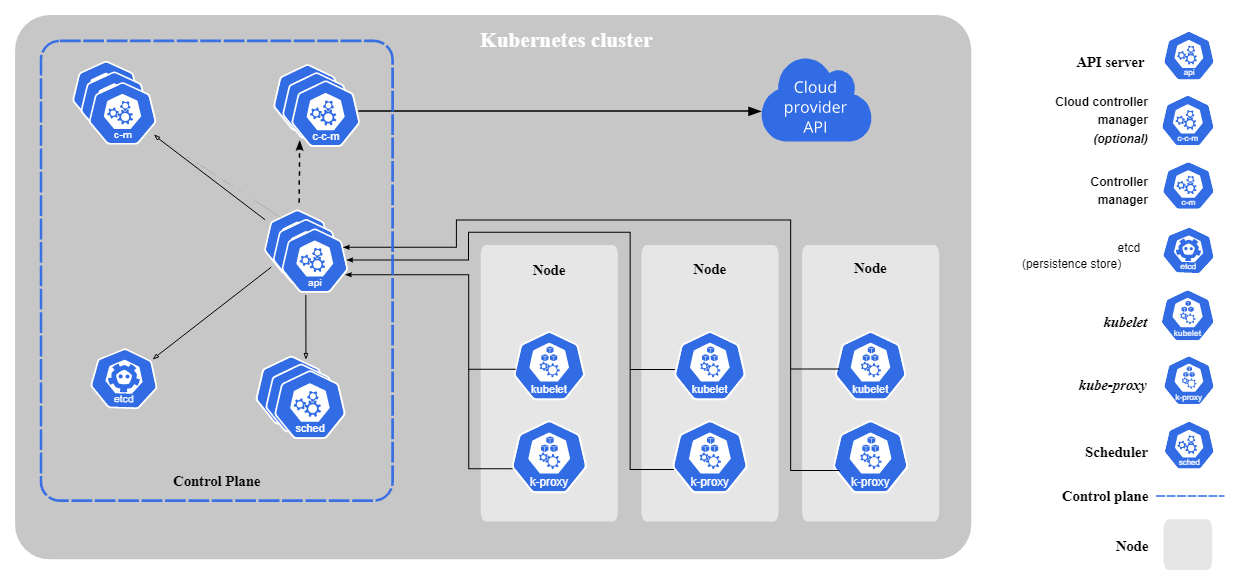
\includegraphics[width=0.7\linewidth]{Pics/kube-architecture}
		\caption{Kiến trúc của Kubernetes}
		\label{fig:kube-architecture}
	\end{figure}
	
	Các thành phần của cụm Kubernetes:\\
	
	\begin{itemize}				
		\item Control Plane: Là trung tâm điều khiển các cụm và làm các cụm kubernetes hoạt động. Đây là nơi quản lý, lên kế hoạch, lập lịch và theo dõi các pod, các node.
		\item Worker Node: Là một máy ảo hoặc máy vật lý chạy Kubernetes. Đây là nơi container thực sự được triển khai để chạy các ứng dụng.
	\end{itemize}
	
	{Các thành phần của Control Plane:\\}
	
	\begin{itemize}				
		\item Kubernetes API server: Nơi mà người dùng và các thành phần khác của Control Plane giao tiếp với nhau.
		\item Scheduler: lập lịch cho các ứng dụng của bạn (chỉ định các workload ví dụ như pods được triển khai ở worker node nào)
		\item  Controller Manager: thực hiện các chức năng cấp cụm, chẳng hạn như nhân bản các thành phần, theo dõi các node, xử lý các node lỗi,...
		\item etcd: một kho dữ liệu phân tán đáng tin cậy lưu trữ cấu hình của các node dưới dạng key value.
	\end{itemize}
	
	{Các thành phần của Worker Node:\\}
	
	\begin{itemize}				
		\item kubelet: dùng để giao tiếp với API server và quản lý các container nằm trong node.
		\item kube-proxy: là một proxy chạy trên các node trong  Kubernetes. kube-proxy duy trì các quy tắc mạng trên các nút. Các quy tắc mạng này cho phép các Pods trong cùng một node hoặc khác node có thể giao tiếp với nhau.
		\item container-runtime: có thể là Docker, rkt, containerd hoặc một loại container-runtime khác.
	\end{itemize}
	
	\subsection{Tổng quan về Pod}
	{\hspace{1cm}Pod là đơn vị thực thi cơ bản của 1 ứng dụng Kubernetes, là đơn vị nhỏ nhất và đơn giản nhất trong mô hình object của Kubernetes. Một Pod đại diện cho các process (tiến trình) chạy trên cluster.\\}
	
	\hspace{0.3cm}Pod đóng gói một container của ứng dụng (hoặc trong một số trường hợp là nhiều container), tài nguyên lưu trữ, một định danh network duy nhất (địa chỉ IP) cũng như các tùy chọn chi phối cách thức các container sẽ chạy. Một Pod đại diện cho một đơn vị triển khai: một instance (phiên bản) của một ứng dụng trong Kubernetes, có thể chứa một container hoặc vài container được liên kết chặt chẽ và chia sẻ tài nguyên.\\
	
	\hspace{0.3cm}Docker là container runtime phổ biến nhất được sử dụng cho Pod trong Kubernetes, tuy nhiên Pods cũng hỗ trợ các container runtime khác. Pod trong Kubernetes cluster có thể được sử dụng theo hai cách chính:\\
	\begin{itemize}				
		\item Pods chạy một container duy nhất. Mô hình “một-container-một-Pod” là trường hợp sử dụng phổ biến nhất của Kubernetes; trong trường hợp này, ta có thể nghĩ về một Pod như một trình bao bọc (đóng gói) xung quanh một container và Kubernetes quản lý các Pod thay vì quản lý trực tiếp các container.
		\item Pods chạy nhiều container cần tương tác với nhau. Một Pod có thể đóng gói một ứng dụng chứa nhiều container cùng hoạt động và được liên kết chặt chẽ với nhau cũng như cần chia sẻ tài nguyên (được gọi là co-located container). Các co-located container này có thể tạo thành một đơn vị dịch vụ gắn kết duy nhất nghĩa là 1 container phục vụ các file từ một volume chia sẻ cho public, trong khi đó, một “sidecar” container khác sẽ làm mới (refresh) hoặc cập nhật các file đó. Pod đóng gói các container và tài nguyên lưu trữ này lại với nhau như một thực thể có thể quản lý được.
	\end{itemize}
	\subsection{Vòng đời của Pod}
	{\hspace{1cm}Giống như các container, Pod được coi là các thực thể tạm bợ, không bền vững(thay vì lâu bền). Các Pod được tạo, gán một ID (UID) duy nhất và được lên lịch cho các node mà chúng vẫn duy trì cho đến khi bị hủy bỏ (theo chính sách khởi động lại) hoặc xóa. Nếu một node chết, các Pod được lập lịch cho node đó sẽ được lập lịch để xóa sau một khoảng thời gian chờ.\\}
	
	\hspace{0.3cm}Pod không tự chữa lành. Nếu một Pod được lên lịch cho một node sau đó không thành công, Pod đó sẽ bị xóa; tương tự như vậy, một Pod sẽ không tồn tại sau khi bị trục xuất do thiếu tài nguyên hoặc bảo trì Node. Kubernetes sử dụng phần trừu tượng cấp cao hơn, được gọi là bộ điều khiển, xử lý công việc quản lý các cá thể Pod tương đối dùng một lần.\\
	
	\hspace{0.3cm}Một Pod nhất định (như được xác định bởi UID) không bao giờ được "lên lịch" đến một nút khác; thay vào đó, Pod đó có thể được thay thế bằng một Pod mới, gần giống, thậm chí có cùng tên nếu muốn, nhưng với một UID khác.\\
	
	\hspace{0.3cm}Giai đoạn của Pod là một bản tóm tắt đơn giản về vị trí của Pod trong vòng đời của nó. Các giai đoạn của Pod:
	\begin{itemize}				
		\item Pending: Pod đã được chấp nhận bởi hệ thống kubernetes, nhưng 1 hoặc vài container image chưa được tạo ra. Nó bao gồm thời gian trước khi được lập lịch cũng như thời gian download image trên mạng về (có thể mất một lúc)
		\item Running: Pod đã được đưa vào 1 node và tất cả các container đã được tạo ra. Ít nhất 1 container vẫn đang chạy hoặc đang ở trong quá trình bắt đầu hoặc khởi động lại.
		\item  Succeeded: Tất cả các container trong pod đã kết thúc thành công và sẽ không được khởi động lại nữa.
		\item  Failed: Tất cả các container trong pod đã kết thúc và ít nhất 1 contrainer đã thất bại trong quá trình kết thúc. Có nghĩa là container đã exited (thoát) với trạng thái non-zero hoặc đã bị kết thúc bởi hệ thống.
		\item  Unknown: Vì một số lý do, trạng thái của pod không thể xác định được, thường là do bị lỗi trong việc giao tiếp với host của pod.
	\end{itemize}
	\subsection{Quản lí pod bằng Workload trên Kubernetes}
	{\hspace{1cm}Workload là một ứng dụng chạy trên Kubernetes. Cho dù workload là một thành phần đơn lẻ hay nhiều thành phần hoạt động cùng nhau, trên Kubernetes, chúng chạy bên trong một tập hợp các pod. Trong Kubernetes, Pod đại diện cho một tập hợp các container đang chạy trên cụm của bạn.\\}
	
	\hspace{0.3cm}Các Pod có một vòng đời xác định. Ví dụ: khi một Pod đang chạy trong cụm thì một lỗi nghiêm trọng trên node nơi pod đó đang chạy có nghĩa là tất cả các pod trên node đó đều bị lỗi. Kubernetes coi mức độ thất bại đó là cuối cùng: bạn sẽ cần tạo một Pod mới để khôi phục, ngay cả khi node sau đó trở lại bình thường.\\
	
	\hspace{0.3cm}Tuy nhiên, để làm cho công việc dễ dàng hơn, các quản trị viên không cần phải quản lý trực tiếp từng Pod. Thay vào đó, có thể sử dụng các workload để quản lý một nhóm các Pod. Các tài nguyên này định cấu hình bộ điều khiển để đảm bảo số lượng phù hợp của loại Pod phù hợp đang chạy, phù hợp với trạng thái đã cấu hình. Kubernetes cung cấp một số workload tích hợp sẵn:
	\begin{itemize}				
		\item Deployment và ReplicaSet (thay thế cho ReplicationController). Deployment rất phù hợp để quản lý workload không trạng thái trên cụm, nơi bất kỳ Pod nào trong Deployment đều có thể hoán đổi cho nhau và có thể được thay thế nếu cần.
		\item StatefulSet là workload API object được dùng để quản lý các ứng dụng stateful (có trạng thái). Nó quản lý việc triển khai và co giãn (scale) các pod và cung cấp sự đảm bảo về thứ tự và tính duy nhất của các pod này.
		\item  Một DeamonSet đảm bảo rằng tất cả hoặc một vài node sẽ chạy 1 bản sao của pod. Khi các node được thêm vào cluster thì pod sẽ được lập lịch vào chúng.
		\item  Job và CronJob xác định các nhiệm vụ chạy đến khi hoàn thành và sau đó dừng lại. Công việc đại diện cho các nhiệm vụ một lần, trong khi CronJobs lặp lại theo lịch trình.
	\end{itemize}
	\section{Một số vấn đề bảo mật kiến trúc Microservices trên Kubernetes}
	{\hspace{1cm}Trong hầu hết các ứng dụng được xây dựng trên cấu trúc monolith, bảo mật được thực thi tập trung và các thành phần riêng lẻ không cần phải lo lắng về việc thực hiện các kiểm tra bảo mật trừ khi có yêu cầu. Kết quả là, mô hình bảo mật của một ứng dụng dựa trên cấu trúc monolith là đơn giản hơn nhiều so với ứng dụng được xây dựng dựa trên cấu trúc microservices. Sau đây là một số vấn đề về bảo mật của kiến trúc Microservices gặp phải.\\}			
	\subsection{Khả năng bị tấn công của các ứng dụng Microservices}
	{\hspace{1cm}Trong một ứng dụng được xây dựng trên cấu trúc monolith, giao tiếp giữa các thành phần bên trong xảy ra trong một tiến trình duy nhất — ví dụ: trong một ứng dụng Java, trong cùng một Máy ảo Java (JVM). Theo kiến trúc microservices, các thành phần bên trong đó được thiết kế dưới dạng các microservices riêng biệt, độc lập và các tiến trình phải gọi lẫn nhau để trao đổi các thông tin. Ngoài ra, mỗi microservice hiện chấp nhận các request một cách độc lập hoặc có các điểm truy cập riêng. Thay vì một vài điểm truy cập, như trong một ứng dụng xây dựng trên cấu trúc monolith, bây giờ  có số lượng các điểm truy cập tăng lên rất lớn. Khi số lượng truy cập vào hệ thống tăng lên, hệ thống sẽ có nhiều điểm bị tấn công hơn. Vấn đề này là một trong những thách thức cơ bản trong việc xây dựng thiết kế bảo mật cho microservices.\\}
	\subsection{Kiểm tra bảo mật làm giảm các hiệu suất}
	{\hspace{1cm}Không giống như trong một ứng dụng được xây dựng trên cấu trúc monolith, mỗi microservice trong triển khai microservices phải thực hiện kiểm tra an ninh độc lập. Từ quan điểm của một ứng dụng dựa trên cấu trúc monolith, trong đó việc kiểm tra bảo mật được thực hiện một lần và các request được gửi đến thành phần tương ứng, nhưng đối với các microservice các quản trị viên phải kiểm tra tất các các điểm truy cập của chúng. Ngoài ra, trong khi xác thực các yêu cầu tại mỗi microservice, bạn có thể cần kết nối với dịch vụ mã thông báo bảo mật từ xa (STS). Các kiểm tra bảo mật phân tán, lặp đi lặp lại và kết nối từ xa này có thể làm tăng độ trễ và làm giảm đáng kể hiệu suất của hệ thống.\\}
	
	\hspace{0.3cm}Một số giải quyết vấn đề này bằng cách đơn giản là tin tưởng vào mạng và tránh kiểm tra bảo mật các microservice. Theo thời gian, mạng tin cậy đã trở thành lỗi thời và đang tiến tới các nguyên tắc mạng không tin cậy. Với nguyên tắc mạng không tin cậy, phải thực hiện bảo mật với từng tài nguyên trong mạng. Mọi thiết kế bảo mật microservices phải có hiệu suất tổng thể có thể chấp nhận được.
	\subsection{Sự phức tạp khi triển khai xác thực khởi động giữa các Microservices}
	{\hspace{1cm}Giao tiếp dịch vụ với dịch vụ diễn ra giữa các microservice. Mỗi kênh liên lạc giữa các microservice phải được bảo vệ. Chúng có nhiều tùy chọn, nhưng giả sử rằng các microservice sử dụng chứng chỉ (certificates).\\}
	
	\hspace{0.3cm}Giờ đây, mỗi microservice phải được cấp chứng chỉ (và khóa bí mật tương ứng), chứng chỉ này sẽ sử dụng để xác thực chính nó với một microservice khác trong quá trình tương tác giữa dịch vụ với dịch vụ. Microservice của người nhận phải biết cách xác thực chứng chỉ được liên kết với microservice đang gọi. Do đó cần một cách để tin tưởng bootstrap giữa các microservices. Ngoài ra cần có khả năng thu hồi chứng chỉ (trong trường hợp khóa bí mật tương ứng bị xâm phạm) và cấp các chứng chỉ mới (thay đổi chứng chỉ định kỳ để giảm thiểu mọi rủi ro khi vô tình làm mất chìa khóa). Những tác vụ này rất cồng kềnh và trừ khi các quản trị viên tìm ra cách tự động hóa chúng.\\
	\subsection{Khó theo dõi các request của các microservice}
	{\hspace{1cm}Khả năng giám sát là thước đo những gì có thể suy ra về trạng thái bên trong của một hệ thống dựa trên kết quả đầu ra bên ngoài của nó. Nhật ký (logs), chỉ số (metrics) và dấu vết (traces) được coi là ba trụ cột của khả năng giám sát.\\}
	
	\hspace{0.3cm}Nhật ký có thể là bất kỳ sự kiện nào bạn ghi lại tương ứng với một dịch vụ nhất định.\\
	
	\hspace{0.3cm}Tổng hợp một tập hợp các nhật ký có thể tạo ra các chỉ số. Theo một cách nào đó, các chỉ số phản ánh trạng thái hệ thống. Ví dụ về mặt bảo mật, các yêu cầu truy cập không hợp lệ trung bình mỗi giờ là một chỉ số.\\
	
	\hspace{0.3cm}Dấu vết cũng dựa trên nhật ký nhưng cung cấp một góc nhìn khác về hệ thống. Theo dõi giúp bạn theo dõi một yêu cầu từ điểm mà nó đi vào hệ thống đến chỉ nơi nó rời khỏi hệ thống. Quá trình này trở nên khó khăn trong mô hình microservices. Không giống như trong một ứng dụng theo cấu trúc monolith, một yêu cầu triển khai microservices có thể xâm nhập vào hệ thống thông qua một microservice và trải dài trên nhiều microservices trước khi nó rời khỏi hệ thống.			
	\subsection{Tính bất biến của container làm việc xác thực và chính sách kiểm soát truy cập của các dịch vụ khó khăn}
	{\hspace{1cm}Máy chủ không thay đổi trạng thái sau khi quay được gọi là máy chủ bất biến. Các mô hình triển khai phổ biến nhất cho microservices là dựa trên container. Mỗi microservice chạy bằng container riêng của nó và tất nhiên, container phải là một máy chủ bất biến. Nói cách khác, sau khi container khởi động, nó sẽ không thay đổi bất kỳ tệp nào trong hệ thống tệp của nó hoặc duy trì bất kỳ trạng thái của nó không thay đổi lúc nó đang chạy.\\}
	
	\hspace{0.3cm}Tính bất biến có tác động gì đến bảo mật và tại sao khái niệm máy chủ bất biến lại được coi là thách thức bảo mật microservices? Trong kiến trúc bảo mật microservices, mỗi microservice trở thành một điểm cần được bảo mật. Do đó, cần duy trì danh sách các máy khách được phép (có thể là các microservice khác) có thể truy cập vào microservice này và cần một bộ chính sách kiểm soát truy cập. Những danh sách này không tĩnh; và cần được phép cập nhật các danh sách này. Nhưng với tính chất bất biến của container, các quản trị viên không thể update hệ thống tệp trong các container của các microservice.
	\subsection{Kiến trúc đa ngôn ngữ đòi hỏi các developer phải có thêm nhiều kiến thức bảo mật hơn}
	{\hspace{1cm}Trong triển khai microservices, các dịch vụ nói chuyện với nhau qua mạng. Họ không phụ thuộc vào việc triển khai từng dịch vụ, mà phụ thuộc vào giao diện dịch vụ. Tình huống này cho phép mỗi microservice chọn ngôn ngữ lập trình của riêng mình và nền tảng công nghệ để triển khai. Trong một môi trường, trong đó mỗi đội development triển khai các mircoservice của riêng mình, mỗi nhóm có thể linh hoạt để chọn các stack công nghệ để phù hợp với sản phẩm. Kiến trúc này, cho phép các các thành phần trong hệ thống để chọn công nghệ tốt nhất cho chúng, được gọi là một kiến trúc đa ngôn ngữ.\\}
	
	\hspace{0.3cm}Một kiến trúc đa ngôn ngữ làm cho vấn đề bảo mật trở nên khó khăn. Bởi vì các đội khác nhau sử dụng các stack công nghệ khác nhau để phát triển, mỗi nhóm phải có các chuyên gia bảo mật riêng. Các chuyên gia này phải chịu trách nhiệm xác định các phương pháp bảo mật tốt nhất và hướng dẫn, nghiên cứu các công cụ bảo mật cho mỗi stack công nghệ để phân tích mã nguồn tĩnh và thử nghiệm động và tích hợp các công cụ đó vào quá trình xây dựng. Trách nhiệm của một nhóm bảo mật tập trung, nhưng bây giờ chia vào các đội development. Điều này làm cho các đội development không chú tâm vào việc phát triển sản phẩm mà phải lo một phần về bảo mật nữa làm cho chất lượng sản phẩm giảm do phải viết các module bảo mật làm cho mã nguồn bị rối và khó đọc.
	
	\newpage				
	\section*{Kết luận Chương 1}
	\addcontentsline{toc}{section}{Kết luận chương 1}
	\hspace{1cm}Như vậy trong chương một em đã nêu ra những thông tin cơ về những công nghệ cũng như kiến trúc của tương lai - Container và Microservices. Đưa ra những ưu điểm cũng như thách thức trong việc triển khai, sử dụng những công nghệ này trong thực tế. Đồng thời cũng nêu ra một hệ thống tự động hoá triển khai, mở rộng và quản lý của công nghệ Container là Kubernetes. Qua việc hiểu tổng quan của các công nghệ trên, em đã nhận ra một số vấn đề bảo mật của kiến trúc Microservices như nguy cơ bị tấn công cao khi mở rộng, việc ảnh hưởng đến hiệu suất khi triển khai bảo mật phân tán cũng như sự phức tạp, khó khăn khi triển khai các giải pháp an toàn cũng yêu cầu nhiều kiến thức đối với những nhà phát triển. Sau đây em sẽ trình bày một giải pháp để có thể giải quyết những vấn đề nói trên.
	
	\chapter{Giới thiệu về HashiCorp Consul}
	
	\section{Tổng quát về Service Mesh}
	
	\hspace{1.0cm}{Để bắt đầu hành trình khám phá service mesh, có ba điều mà chúng ta cần phải biết: Service Mesh là gì, cách thức nó hoạt động như nào và tại sao chúng ta lại sử dụng nó. Có lẽ, để định nghĩa ngắn gọn service mesh, thì chúng ta có thể hiểu như sau:\\
	
	\hspace{0.3cm}{Service mesh là lớp kiến trúc hạ tầng mà cho phép kiểm soát giao tiếp mạng của hệ thống từ một control plan duy nhất.\\}
	
	\hspace{-0.8cm}Để hiểu hơn về định nghĩa trên, chúng ta cần chia thành các phần sau:\\
	
	\hspace{0.3cm}{Thông qua lớp kiến trúc hạ tầng, service mesh không phải là một phần của service, nó được triển khai và vận hành theo một cách độc lập. Vì nó không thể xác định được cụ thể được logic hoạt động của dịch vụ cụ thể, nhưng nó ảnh hưởng đến mọi dịch vụ, nên nó được coi là cơ sở hạ tầng hoặc phần mềm trung gian.\\}
	
	\hspace{0.3cm}{Dưới đây là hình ảnh của một phần mềm thông thường. Dịch vụ và ứng dụng chạy trên các cơ sở hạ tầng. Service mesh nằmg ở lớp cơ sở hạ tầng đầu tiên với các yêu cầu về lưu trữ, metrics và cơ sở hạ tầng cao cấp khác. Bến dưới đó là Kubernetes, máy ảo hoặc bất kì kiến trúc máy tính nào mà có thể chạy. Bên dưới cùng là phần cứng (bare metal)\\}
	
	\begin{figure}[h]
		\centering
		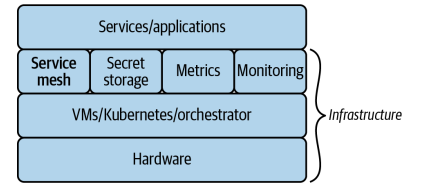
\includegraphics[width=0.7\linewidth]{Pics/software_stack}
		\caption{\label{fig:software_stack} Một khối ứng dụng cụ thể}
		\label{fig:software_stack}
	\end{figure}
	
	\subsection{Phương thức hoạt động của service mesh}
	\hspace{1.0cm}{Service mesh được tạo thành từ các proxy sidecar và control plan.}
	\subsubsection{Proxy Sidecar}
	\hspace{1.0cm}{Proxy là một ứng dụng mà lưu lượng truy cập được định tuyến trên đường đến đích của nó. Các proxy phổ biến mà chúng ta có thể đã nghe nói đến là NGINX, HAProxy và Envoy. Trong hầu hết các service mesh, tất cả lưu lượng dịch vụ (vào và ra) được định tuyến thông qua một proxy cục bộ dành riêng cho từng phiên bản dịch vụ\\}
	
	\hspace{0.3cm}{Hình bên dưới thể hiện service mesh sẽ như thế nào với 2 đối tượng: frontend và backend. Khí frontend gọi đến backend, proxy cục bộ của frontend sẽ bắt tất cả các yêu cầu được đi ra ngoài. Proxy của frontend sẽ chuyển các yêu cầu đến dịch vụ backend. Khi mà yêu cầu được đưa tới dịch vụ backend, tiếp tục, nó được proxy cục bộ của backend nắm bắt và kiểm tra. Nếu yêu cầu được cho phép, proxy của backend sẽ chuyển tiếp yêu cầu đó đên dịch vụ backend thực tế.\\}
	\begin{figure}[h]
		\centering
		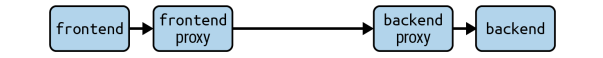
\includegraphics[width=0.7\linewidth]{Pics/proxy}
		\caption{\label{fig:proxy} Hai ứng dụng giao tiếp với nhau thông qua service mesh}
		\label{fig:proxy}
	\end{figure}
	
	\hspace{0.3cm}{Mỗi phiên bản của một dịch vụ phải được triển khai với proxy cục bộ của chính nó. Mẫu triển khai ứng dụng trợ giúp - trong trường hợp này là proxy - cùng với dịch vụ chính được gọi là mẫu sidecar và do đó, proxy cục bộ được gọi là proxy sidecar.\\}
	
	\hspace{0.3cm}{Proxy Sidecar là một thành phần quan trọng của service mesh vì chúng cho phép kiểm soát lưu lượng dịch vụ mà không cần sửa đổi hoặc triển khai lại các dịch vụ cơ bản. Vì proxy sidecar chạy dưới dạng các quy trình riêng biệt với dịch vụ nên chúng có thể được cấu hình lại mà không ảnh hưởng đến dịch vụ. Ví dụ: proxy sidecar của dịch vụ backend có thể được cấu hình lại để từ chối lưu lượng truy cập từ dịch vụ backend mà không cần thay đổi mã hoặc triển khai lại chính dịch vụ backend.}
	
	\subsubsection{Control Plane}
	\hspace{1.0cm}{Công việc của control plane là quản lý và định cấu hình các proxy sidecar. Như chúng ta có thể thấy hình bên dưới, control plane là một dịch vụ riêng biệt phải được triển khai riêng; nó không được triển khai như một sidecar. control plane là nơi chứa hầu hết logic phức tạp của service mesh: nó phải theo dõi các dịch vụ bắt đầu và dừng, ký và phân phối chứng chỉ, cấu hình lại proxy, v.v. Bản thân các proxy sidecar tương đối đơn giản: chúng nhận cấu hình từ control plane nêu chi tiết những hành động nào sẽ thực hiện trên lưu lượng truy cập và họ thực hiện những hành động đó.}
	\begin{figure}[h]
		\centering
		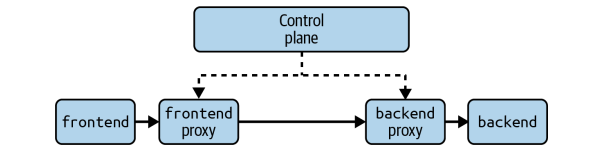
\includegraphics[width=0.7\linewidth]{Pics/control-plane}
		\caption{\label{fig:control-plane} Control plane quản lý các sidecar proxy.}
		\label{fig:control-plane}
	\end{figure}

	\subsection{Các tính năng của service mesh}
	\hspace{1.0cm}{Service mesh cung cấp các tính năng trong bốn lĩnh vực: bảo mật, khả năng quan sát, độ tin cậy và kiểm soát lưu lượng. Đề xuất giá trị cơ bản của service mesh là khả năng cung cấp các tính năng này trên mọi dịch vụ và khối lượng công việc mà không cần sửa đổi mã dịch vụ.}
	\subsubsection{Bảo mật}
	\hspace{1.0cm}{Một trong những lý do chính khiến các công ty triển khai service mesh là để bảo mật mạng của họ. Thông thường, điều này có nghĩa là mã hóa lưu lượng giữa tất cả các khối lượng công việc và triển khai xác thực cũng như ủy quyền.\\}
	
	\hspace{0.3cm}{Giải quyết vấn đề này có thể rất khó khăn trong kiến trúc microservices mà không có service mesh. Yêu cầu mã hóa mọi yêu cầu có nghĩa là cung cấp chứng chỉ bảo mật tầng vận chuyển (TLS) cho mọi dịch vụ theo cách an toàn và quản lý cơ sở hạ tầng ký chứng chỉ của riêng mình. Xác thực và ủy quyền mọi yêu cầu có nghĩa là cập nhật và duy trì mã xác thực trong mọi dịch vụ.\\}
	
	\hspace{0.3cm}{Service mesh giúp công việc này dễ dàng hơn nhiều vì nó có thể cấp chứng chỉ và định cấu hình proxy sidecar để mã hóa lưu lượng và thực hiện ủy quyền - tất cả mà không có bất kỳ thay đổi nào đối với các dịch vụ cơ bản\\}
	
	\begin{figure}[h]
		\centering
		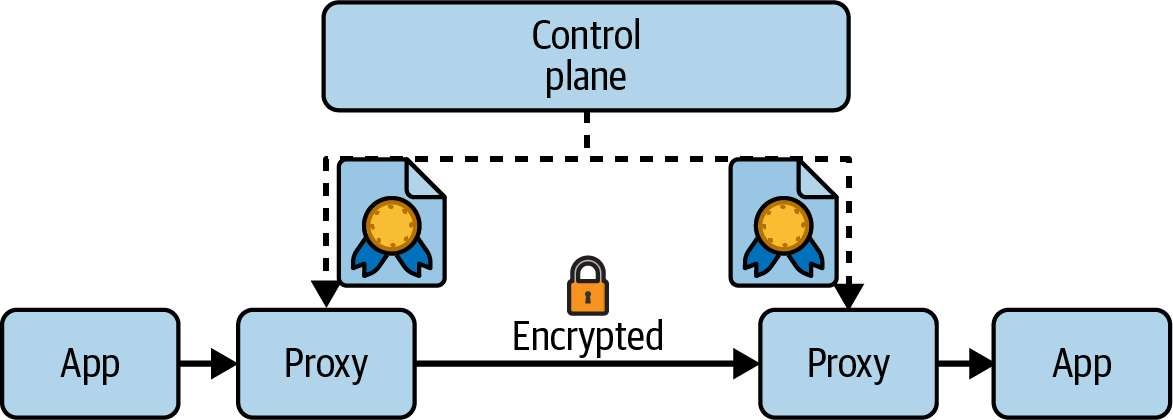
\includegraphics[width=0.7\linewidth]{Pics/service-mesh_encrypted}
		\caption{\label{fig:service-meshencrypted} Service mesh phát hành chứng chỉ và mã hóa đường truyền. }
		\label{fig:service-meshencrypted}
	\end{figure}

	\subsubsection{Khả năng quan sát}
	\hspace{1cm}{Khả năng quan sát là khả năng hiểu điều gì đang xảy ra với các dịch vụ khi chúng đang chạy. Dữ liệu về khả năng quan sát là cần thiết để hiểu kiến trúc vi dịch vụ và chẩn đoán lỗi, nhưng việc định cấu hình tất cả các dịch vụ để phát ra các chỉ số và dữ liệu khác theo cách thống nhất có thể là một thách thức.\\}
	
	\hspace{0.3cm}{Nắm bắt dữ liệu quan sát được là công việc hoàn hảo cho service mesh vì tất cả các yêu cầu đều chảy qua proxy của nó. Service mesh có thể định cấu hình proxy của nó để phát ra số liệu trên tất cả các dịch vụ ở định dạng nhất quán mà không cần sửa đổi hoặc triển khai lại các dịch vụ cơ bản.}
	
	\subsubsection{Độ tin cậy}
	\hspace{1cm}{Trong các hệ thống phân tán, thường có lỗi xảy ra. Xây dựng các hệ thống phân tán đáng tin cậy có nghĩa là giảm thiểu sự cố nếu có thể và xử lý sự cố một cách khéo léo khi nó chắc chắn xảy ra.\\}
	
	\hspace{0.3cm}{Giảm thất bại có thể có nghĩa là thực hiện kiểm tra tình trạng để lưu lượng truy cập chỉ được gửi đến các dịch vụ khỏe mạnh. Xử lý lỗi có thể có nghĩa là thử lại các yêu cầu không thành công hoặc triển khai thời gian chờ, vì vậy một dịch vụ không chờ phản hồi mãi mãi.\\}
	
	\hspace{0.3cm}{Việc triển khai các kỹ thuật này trong mã tốn nhiều thời gian, dễ xảy ra lỗi và khó thực hiện một cách nhất quán trên tất cả các dịch vụ. Với service mesh, proxy có thể thực hiện các kỹ thuật này cho bất kỳ dịch vụ nào - tất cả những gì chúng ta cần làm là tương tác với control plane. Chúng ta cũng có thể điều chỉnh cài đặt theo thời gian thực khi tải dịch vụ thay đổi.\\}
	
	\begin{figure}[h]
		\centering
		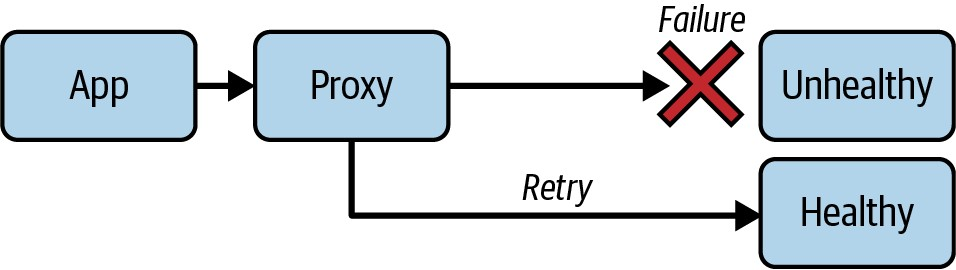
\includegraphics[width=0.7\linewidth]{Pics/reliability}
		\caption{\label{fig:reliability} Service mesh có thể được cấu hình để thử lại các yêu cầu không thành công cho các trường hợp khác.}
		\label{fig:reliability}
	\end{figure}
	
	\subsubsection{Kiểm soát lưu lượng}
	\hspace{1cm}{Kiểm soát lưu lượng là về việc kiểm soát nơi lưu lượng giữa các dịch vụ được định tuyến. Kiểm soát lưu lượng giải quyết nhiều vấn đề:}
	
	\begin{itemize}
		\item Triển khai các chiến lược triển khai, chẳng hạn như triển khai canary, trong đó một lượng nhỏ  lưu lượng truy cập "canary" được chuyển đến phiên bản mới của dịch vụ để xem liệu dịch vụ đó có hoạt động hay không trước khi triển khai đầy đủ phiên bản mới.
		\smallskip
		\item Di chuyển từ nguyên khối sang vi dịch vụ, trong đó các dịch vụ được tách ra khỏi nguyên khối và lưu lượng truy cập trước đây được định tuyến đến nguyên khối được định tuyến lại một cách liền mạch đến các microservice mới.
		\smallskip
		\item Chuyển đổi dự phòng đa cụm, trong đó lưu lượng được định tuyến đến các dịch vụ trong cụm lành mạnh khác nếu cụm cục bộ ngừng hoạt động.
	\end{itemize}

	\subsubsection{Tính năng kết hợp}
	\hspace{1cm}{Bây giờ các loại tính năng mà service mesh cung cấp là về bảo mật, khả năng quan sát, độ tin cậy và kiểm soát lưu lượng. Một mình, các tính năng này rất hữu ích, nhưng chúng thậm chí còn mạnh mẽ hơn khi kết hợp.\\}
	
	\hspace{0.3cm}{Ví dụ: dữ liệu về khả năng quan sát được cung cấp bởi service mesh có thể được kết hợp với các tính năng kiểm soát lưu lượng và độ tin cậy. Nếu lưới phát hiện ra rằng một phiên bản dịch vụ đang trả về lỗi, nó có thể chuyển hướng lưu lượng truy cập đến các phiên bản khỏe mạnh hoặc một cụm hoàn toàn khác. Hoặc các tính năng bảo mật dạng lưới có thể được kết hợp với các tính năng có thể quan sát để phát hiện khi một dịch vụ đang cố thực hiện các yêu cầu mà dịch vụ đó không được phép thực hiện - có khả năng chỉ ra một vi phạm bảo mật. Khi chúng ta tự triển khai Consul, chúng ta sẽ thấy nhiều trường hợp sử dụng mà chúng ta có thể kết hợp các tính năng service mesh.\\}
	
	\hspace{0.3cm}{Nếu tổ chức cần những tính năng này, thì chúng ta phải quyết định xem nó có xứng đáng với độ phức tạp bổ sung của service mesh hay không hay liệu chúng ta có nên triển khai chúng trong mã dịch vụ hay không. Chìa khóa để trả lời câu hỏi đó là kiểm tra quy mô tổ chức.\\}
	
	\subsection{Khi nào nên sử dụng service mesh}
	\hspace{1cm}{Không còn nghi ngờ gì nữa, việc triển khai service mesh sẽ làm tăng thêm độ phức tạp. Bây giờ chúng ta có proxy sidecar và control plane service mesh để quản lý. Ngoài ra, chúng ta sẽ cần nhiều tài nguyên điện toán hơn (CPU và bộ nhớ) để chạy proxy và control plane, và giờ đây, tất cả lưu lượng truy cập sẽ mất thêm một bước nhảy qua các proxy sidecar cục bộ, điều này làm tăng thêm độ trễ. Việc triển khai các tính năng service mesh trong mã sẽ tiết kiệm tài nguyên và giảm độ phức tạp của cơ sở hạ tầng (mặc dù nó sẽ làm tăng độ phức tạp của mã). Để một service mesh xứng đáng, nó phải cung cấp nhiều giá trị cho tổ chức.\\}
	
	\hspace{0.3cm}{Một công thức đơn giản để biết khi nào nên sử dụng service mesh là khi chúng ta (a) cần giải quyết các vấn đề về mạng trong các lĩnh vực đã nêu trước đó (bảo mật, khả năng quan sát, độ tin cậy và kiểm soát lưu lượng) và (b) tổ chức của chúng ta ở quy mô lớn, hoặc sẽ sớm đạt đến quy mô mà việc giải quyết những vấn đề đó trong mã dịch vụ là quá tốn kém.\\}
	
	\hspace{0.3cm}{Ví dụ: giả sử tổ chức đang chuyển sang kiến trúc bảo mật không tin cậy, trong đó tất cả lưu lượng truy cập nội bộ được mã hóa, xác thực và ủy quyền. Nếu hệ thống chỉ chạy hai dịch vụ, chúng ta có thể dễ dàng mã hóa lại các dịch vụ đó. Tuy nhiên, nếu hệ thống đang chạy 400 dịch vụ, thì chúng ta sẽ không thể mã hóa lại tất cả các dịch vụ đó trong một khoảng thời gian hợp lý. Trong trường hợp này, một service mesh có rất nhiều ý nghĩa.\\}
	
	\hspace{0.3cm}{Ngoài ra, ở một quy mô nhất định, sẽ có các dịch vụ và khối lượng công việc mà chúng ta muốn kiểm soát mà chúng ta thực sự không có khả năng chỉnh sửa mã của chúng. Ví dụ: có thể tổ chức đang triển khai một phần mềm nguồn mở được đóng gói hoặc có thể tổ chức đang sử dụng cơ sở dữ liệu do đám mây quản lý. Lý tưởng nhất là chúng ta sẽ có cùng quyền kiểm soát đối với những khối lượng công việc mà chúng ta thực hiện đối với các dịch vụ khác của mình.\\}

	\section{Giới thiệu về Consul}
	
	\hspace{1.0cm}{Khi Consul lần đầu tiên xuất hiện vào năm 2014. Điện toán đám mây và kiến trúc hướng dịch vụ (tiền thân của vi dịch vụ) đang trở thành xu hướng chủ đạo và mọi công ty bắt đầu vật lộn với vấn đề làm thế nào để định tuyến đến các dịch vụ và xử lý lỗi trong một hệ thống phân phối.\\}
	
	\hspace{0.3cm}{Consul là một công nghệ mang tính cách mạng vì nó kết hợp khám phá dịch vụ dựa trên DNS với một hệ thống phát hiện lỗi mạnh mẽ. Một dịch vụ sẽ đăng ký vào Consul và các dịch vụ khác có thể sử dụng mục nhập DNS của Consul để định tuyến đến nó. Ví dụ: dịch vụ giao diện người dùng sẽ có sẵn tại frontend.service.consul. Consul cũng phát hiện lỗi bằng cách sử dụng một thuật toán buôn chuyện có tên là Serf (được đề cập ở phần sau của chương này) và kiểm tra sức khỏe. Nếu một nút hoặc dịch vụ gặp sự cố, Consul sẽ nhanh chóng nhận thấy và xóa nó khỏi DNS.\\}
	
	\hspace{0.3cm}{Consul là mã nguồn mở, miễn phí sử dụng và giải quyết vấn đề mà hàng nghìn công ty gặp phải một cách tinh tế. Ngành công nghiệp nhanh chóng áp dụng nó.\\}
	
	\hspace{0.3cm}{Theo thời gian, kiến trúc hướng dịch vụ ngày càng lớn hơn và trở thành kiến trúc microservice với các dịch vụ ngày càng nhỏ hơn. Điều này dẫn đến sự gia tăng của Docker và bộ điều phối container như Kubernetes. Phong trào microservices và Kubernetes đã thay đổi ngành theo hai cách quan trọng:\\}
	
	\hspace{0.3cm}{Đầu tiên, khám phá dịch vụ DNS không còn đủ nữa. Các nhà phát triển cần nhiều tính năng làm việc trên mạng hơn về bảo mật, khả năng quan sát, độ tin cậy và kiểm soát lưu lượng để giúp chạy tất cả các dịch vụ này. Việc triển khai các tính năng này trong mã dịch vụ cũng trở nên khó khăn hơn vì số lượng dịch vụ không ngừng tăng lên.\\}
	
	\hspace{0.3cm}{Thứ hai, Kubernetes giúp việc chạy sidecar proxy trở nên dễ dàng hơn nhiều nhờ vào mô hình nhóm, trong đó nhiều vùng chứa có thể chạy cùng nhau trong một mạng riêng (Trước đây, có thể chạy hai quy trình cùng nhau, tuy nhiên, điều đó khó khăn hơn vì chúng ta cần phải sắp xếp việc triển khai và cấu hình của chúng theo cách thủ công. Ngoài ra, các quy trình khác trên cùng một máy có thể truy cập cùng một mạng và hệ thống tệp.)\\}
	
	\hspace{0.3cm}{Những thay đổi này đã kích hoạt công nghệ service mesh như chúng ta biết ngày nay.\\}
	
	\hspace{0.3cm}{Nhóm Consul tại HashiCorp đã đi theo những xu hướng này và vào năm 2018, họ đã phát hành một tính năng service mesh có tên là Consul Connect. Consul Connect tập trung vào liên lạc an toàn giữa các dịch vụ và hỗ trợ thêm cho các proxy sidecar để mã hóa lưu lượng giữa các dịch vụ. Kể từ đó, Consul đã phát triển thành một mạng service mesh đầy đủ chức năng với các tính năng không chỉ liên quan đến liên lạc an toàn mà còn cả khả năng quan sát, độ tin cậy và kiểm soát lưu lượng.\\}
	
	\hspace{0.3cm}{Bỏ qua lịch sử đó, chúng ta đã sẵn sàng tìm hiểu về cách thức hoạt động của Consul và điều gì làm cho nó trở nên độc đáo với tư cách là một mạng service mesh. Các phần sau đây đề cập đến kiến trúc của Consul và các giao thức mà nó sử dụng để duy trì độ tin cậy và khả năng mở rộng.\\}
	
	\subsection{Kiến trúc}
	\hspace{1cm}{Một bản cài đặt Consul được tạo thành từ ba bộ thành phần: máy chủ Consul, ứng dụng client Consul và proxy sidecar. Các proxy Sidecar nói chuyện với các client Consul local của họ và các client Consul nói chuyện với các máy chủ Consul. Thường có ba hoặc năm Node máy chủ Consul  và có thể có tới hàng nghìn Node khối lượng công việc.\\}
	
	\begin{figure}[h]
		\centering
		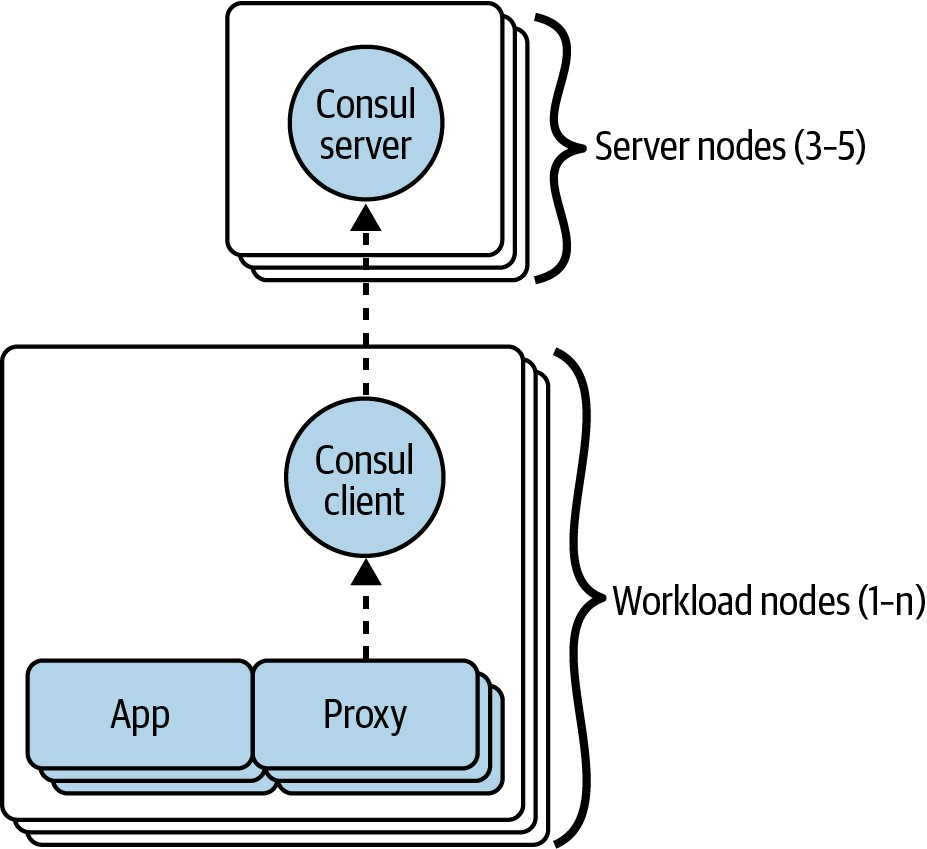
\includegraphics[width=0.7\linewidth]{Pics/architecture}
		\caption{\label{fig:architecture} Bản cài đặt Consul bao gồm máy chủ Consul, máy client Consul và proxy sidecar.}
		\label{fig:architecture}
	\end{figure}
	
	\hspace{0.3cm}{Để liên kết kiến trúc của Consul với kiến trúc của service mesh chung thì các máy chủ và client của Consul là một phần của control plane.}
	
	\subsubsection{Máy chủ Consul}
	\hspace{1cm}{Máy chủ Consul là cơ sở dữ liệu của Consul. Consul cần lưu trữ dữ liệu như danh mục (danh sách các nút và dịch vụ), cấu hình, trạng thái sức khỏe, v.v. Để triển khai sản xuất Consul, chúng ta phải chạy nhiều máy chủ Consul (mặc dù với mục đích thử nghiệm, một máy chủ là đủ). Việc chạy nhiều máy chủ đảm bảo tính sẵn sàng cao và tính ổn định của dữ liệu: nếu một máy chủ gặp sự cố, các máy chủ còn lại vẫn có thể phục vụ các yêu cầu và không có dữ liệu nào bị mất.\\}

	\hspace{0.3cm}{chúng ta phải luôn chạy số lượng máy chủ lẻ - ví dụ: ba hoặc năm - vì chạy số lượng máy chủ chẵn không làm tăng khả năng chịu lỗi của Consul (và do đó, thêm máy chủ gây lãng phí tài nguyên). Consul phải có đa số trong số các máy chủ đang chạy để tiếp tục hoạt động mà không gặp sự cố (Nếu phần lớn các máy chủ không chạy, Consul sẽ “lỗi tĩnh”. Điều này có nghĩa là mọi thứ sẽ tiếp tục hoạt động, nhưng không có thay đổi nào (chẳng hạn như đăng ký dịch vụ mới) có thể được thực hiện). Nếu chúng ta đang chạy ba máy chủ, phần lớn là hai máy chủ, vì vậy chúng ta có thể chấp nhận một máy chủ bị hỏng. Nếu chúng ta đang chạy bốn máy chủ, phần lớn là ba máy chủ, vì vậy chúng ta vẫn chỉ có thể chấp nhận một máy chủ bị hỏng.\\}
	
	\hspace{0.3cm}{Máy chủ Consul lưu trữ dữ liệu của họ trên đĩa. Trên Kubernetes, các máy chủ Consul được triển khai dưới dạng StatefulSet và sử dụng PersistentVolume để lưu trữ dữ liệu của chúng:}
	
	\begin{itemize}
		\item \textbf{StatefulSet}
		\subitem Một loại tài nguyên Kubernetes tương tự như Deployment (loại tài nguyên Kubernetes được sử dụng để triển khai nhiều bản sao của một dịch vụ và quản lý vòng đời của nó) đảm bảo cùng một khối lượng lưu trữ luôn được ghép nối với cùng một Pod.
		\smallskip
		\item \textbf{PersistentVolume}
		\subitem Một đoạn dung lượng lưu trữ có thể được gắn vào một pod nhưng sẽ không bị xóa nếu pod đó khởi động lại.
	\end{itemize}
	
	\hspace{0.3cm}{Trên máy ảo, máy chủ Consul nên được triển khai với ổ đĩa sẽ không bị mất khi Node khởi động lại.\\}
	
	\hspace{0.3cm}{Đối với sản xuất, chúng ta nên dành toàn bộ một Node cho từng máy chủ Consul để tránh các sự cố tranh chấp tài nguyên. Trên Kubernetes, điều này có thể được thực hiện bằng cách có một nhóm Node riêng biệt sử dụng các taint và dung sai để hạn chế Pod nào có thể được lên lịch cho các Node đó.}
	
	\subsubsection{Client Consul}
	\hspace{1cm}{Client Consul chạy trên mọi Node khối lượng công việc trong cụm (Nếu chúng ta có các Node dành riêng cho máy chủ Consul, thì các Node khác trong cụm của chúng ta sẽ chạy các dịch vụ thực tế và các ứng dụng là các Node khối lượng công việc.) Client Consul chịu trách nhiệm phát hiện tình trạng của các dịch vụ đang chạy trên Node của chúng và tình trạng của các Node khác trong cụm. Các client Consul sau đó gửi thông tin này đến các máy chủ Consul để cập nhật danh mục của họ.\\}
	
	\hspace{0.3cm}{Về lý thuyết, máy chủ Consul có thể kiểm tra tình trạng của tất cả các dịch vụ và Node trong một cụm và sẽ không cần máy client Consul. Tuy nhiên, trên thực tế, cách tiếp cận tập trung này không thể mở rộng cho hàng chục nghìn Node và dịch vụ mà Consul muốn hỗ trợ. Thay vào đó,việc chạy ứng dụng client Consul trên mỗi Node cho phép Consul sử dụng phương pháp phân tán(Phát hiện lỗi phân tán bằng Serf) kiểm tra tình trạng của dịch vụ và Node dễ dàng mở rộng quy mô và dẫn đến phát hiện lỗi chỉ mất một phần nghìn giây, ngay cả trong các cụm lớn (Trên Kubernetes, việc phát hiện lỗi của Consul là không cần thiết vì Kubernetes thực hiện Node và phát hiện lỗi dịch vụ qua kubelet. Trong các phiên bản tương lai của Consul, ứng dụng client Consul có thể không còn cần thiết trên Kubernetes nữa.)\\}
	
	\hspace{0.3cm}Client Consul cũng chịu trách nhiệm định cấu hình proxy sidecar trên các Node của họ. Điều này được đề cập chi tiết hơn khi tôi xem qua một trường hợp sử dụng ví dụ.\\{}
	
	\hspace{0.3cm}{Máy chủ Consul cũng có thể hoạt động như client Consul. Điều này có nghĩa là chúng ta có thể chạy các dịch vụ trên cùng các Node như máy chủ Consul và các máy chủ sẽ quản lý các proxy sidecar mà không cần phải chạy ứng dụng client Consul. Kiến trúc này chỉ được đề xuất cho các cụm thử nghiệm nhỏ, nơi không hợp lý khi sử dụng các Node riêng cho máy chủ Consul và khối lượng công việc dịch vụ.\\}
	
	\hspace{0.3cm}{Trên Kubernetes, các client Consul được chạy dưới dạng DaemonSet. DaemonSet là loại tài nguyên Kubernetes tương tự như Deployment đảm bảo một nhóm máy client Consul sẽ chạy trên mọi Node trong cụm. Điều này đảm bảo luôn có sẵn ứng dụng client Consul để quản lý các proxy sidecar. Trên máy ảo, chúng ta có trách nhiệm đảm bảo rằng mọi Node khối lượng công việc đều được cung cấp máy client Consul.}
	
	\subsubsection{Proxy Sidecar}
	\hspace{1cm}{Mỗi phiên bản dịch vụ, một phiên bản đang chạy cụ thể của một dịch vụ, có một proxy sidecar chuyên dụng. Trách nhiệm của proxy là chặn các yêu cầu đến và từ phiên bản dịch vụ của nó, đồng thời thực hiện các hành động theo yêu cầu như đã định cấu hình - ví dụ: mã hóa yêu cầu bằng TLS hoặc từ chối yêu cầu từ một số dịch vụ nhất định.\\}
	

	\begin{figure}[h]
		\centering
		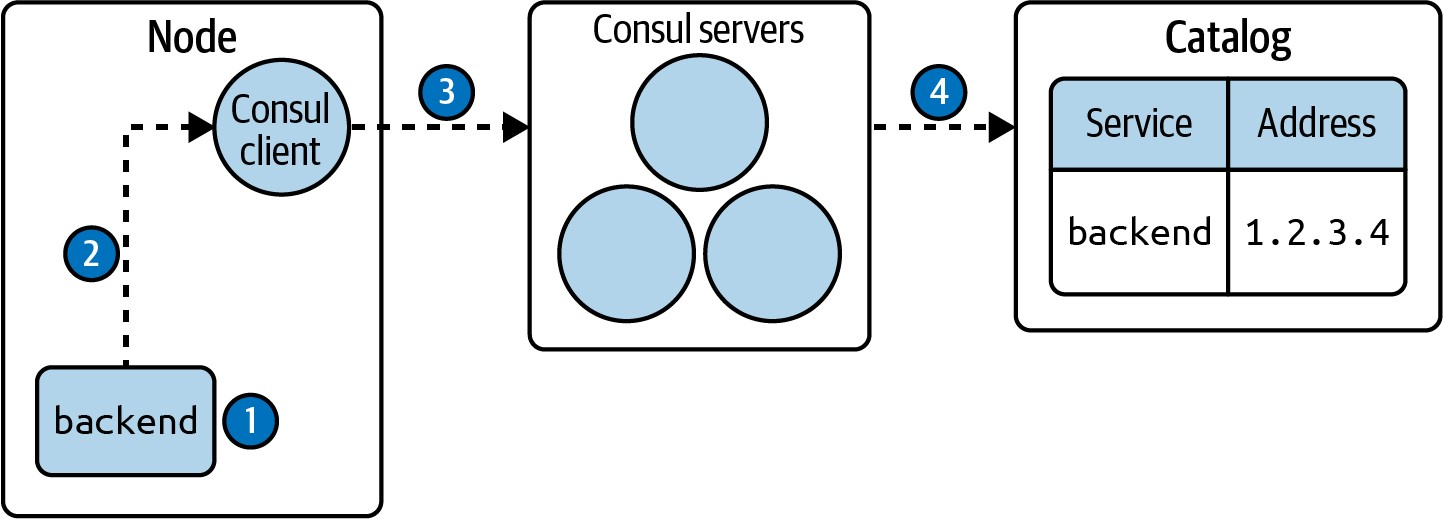
\includegraphics[width=0.7\linewidth]{Pics/example}
		\caption{\label{fig:example} Một dịch vụ mới đang được bắt đầu trên một Node.}
		\label{fig:example}
	\end{figure}

	\hspace{0.3cm}{Consul tự nó không phải là một proxy (Về mặt kỹ thuật, đó là do nó đi kèm với cái được gọi là proxy tích hợp, nhưng proxy này có tối thiểu chức năng và chỉ nên được sử dụng cho các trường hợp thử nghiệm nhỏ) Thay vào đó, Consul sử dụng một proxy gọi là Envoy. Envoy là một proxy nguồn mở được tạo tại Lyft. Nó hiện là một dự án CNCF (Cloud Native Computing Foundation) được nhiều service mesh sử dụng. Envoy được viết bằng C++ cho hiệu năng và có dung lượng bộ nhớ rất thấp. Điều này có nghĩa là nó có thể chạy bên cạnh tất cả các dịch vụ của chúng ta với tác động tối thiểu đến tài nguyên và độ trễ. Envoy hỗ trợ hàng trăm tính năng để cân bằng tải, khả năng quan sát, kiểm tra sức khỏe, v.v. Máy khách Consul định cấu hình Envoy qua API gRPC của nó.\\}

	
	\hspace{0.3cm}{Trên Kubernetes, sidecar proxy chạy dưới dạng các container riêng biệt trong các nhóm dịch vụ. Điều này đảm bảo rằng các bộ chứa dịch vụ có thể định tuyến đến các proxy sidecar của chúng trong mạng nhóm cục bộ. Trên máy ảo, proxy sidecar chạy dưới dạng các quy trình riêng biệt cho từng phiên bản dịch vụ trên máy ảo đó.\\}
	

	\begin{figure}[h]
		\centering
		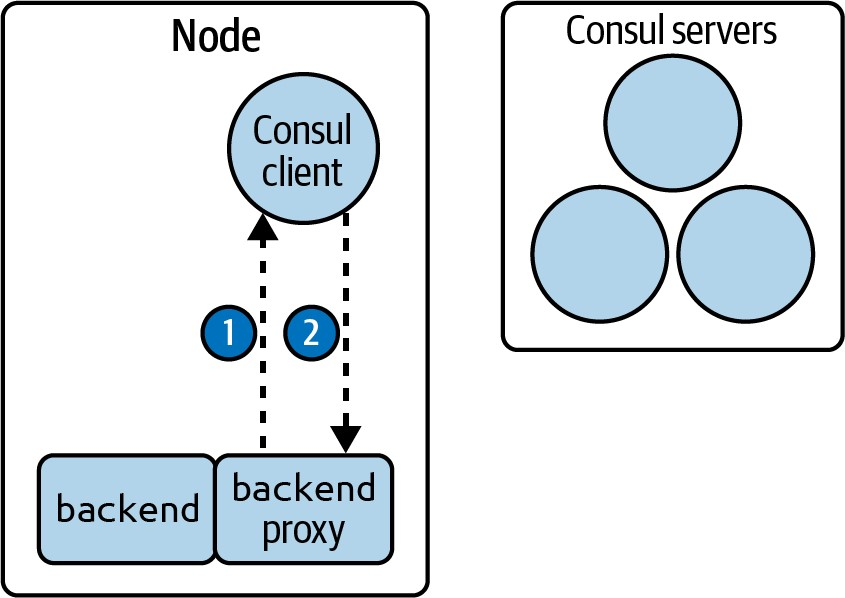
\includegraphics[width=0.7\linewidth]{Pics/example2}
		\caption{\label{fig:example2} Client Consul cấu hình proxy backend.}
		\label{fig:example2}
	\end{figure}

	\hspace{0.3cm}{Bây giờ chúng ta đã quen thuộc với máy chủ Consul, client và proxy sidecar, hãy xem qua một trường hợp sử dụng ví dụ để hiểu cách cả ba thành phần hoạt động cùng nhau.}
	
	\subsubsection{Trường hợp sử dụng ví dụ}
	\hspace{1cm}{Hãy tưởng tượng một dịch vụ mới gọi là backend được bắt đầu trên một Node. Tiếp theo, dịch vụ backend được đăng ký với địa chỉ IP của nó - ví dụ: 1.2.3.4 - vào ứng dụng client Consul trên Node đó (bước 2). Sau đó, ứng dụng client Consul đưa ra yêu cầu quay lại máy chủ Consul để thông báo cho họ biết rằng một dịch vụ mới có tên là backend đang chạy trên Node đó có địa chỉ 1.2.3.4 (bước 3). Các máy chủ Consul sau đó thêm dịch vụ đó vào danh mục (bước 4).\\}
	


	\begin{figure}[h]
		\centering
		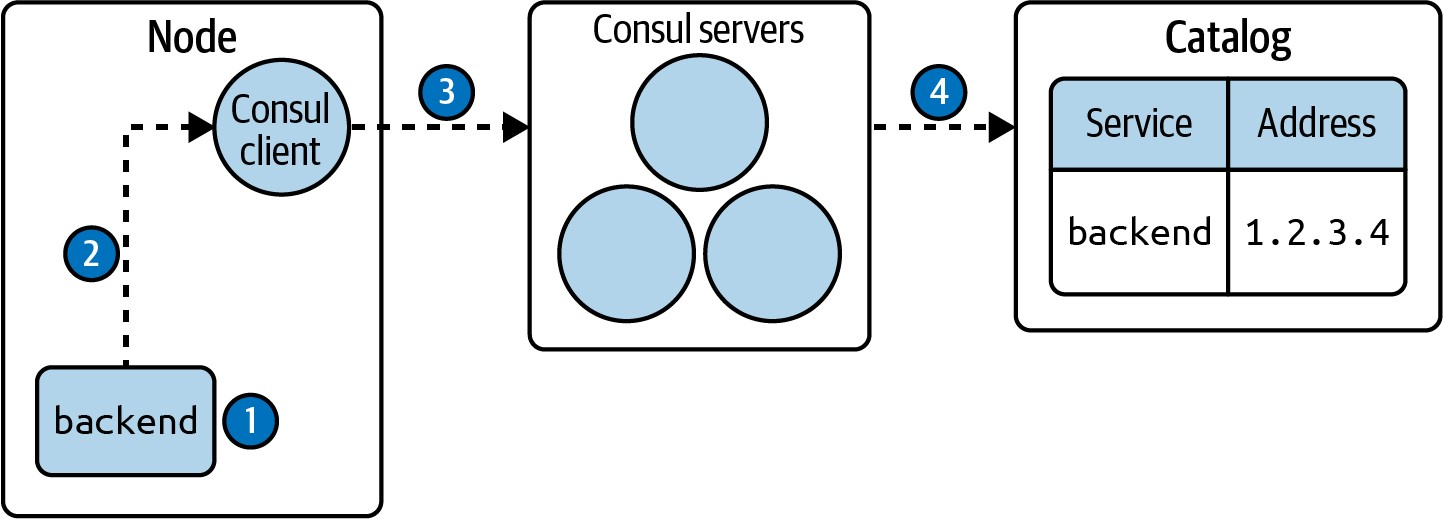
\includegraphics[width=0.7\linewidth]{Pics/example}
		\caption{\label{fig:example} Một dịch vụ mới đang được bắt đầu trên một Node.}
		\label{fig:example}
	\end{figure}
	

	\hspace{0.3cm}{Proxy của giao diện người dùng cần biết địa chỉ của dịch vụ backend để thực hiện yêu cầu. Để thực hiện điều này, ứng dụng client Consul trên cùng một nút với dịch vụ giao diện người dùng sẽ xem danh mục máy chủ Consul để biết các phiên bản mới của dịch vụ backend (bước 1 trong Hình 2.10). Khi một phiên bản mới của dịch vụ backend được đăng ký vào danh mục, máy chủ Consul sẽ gửi địa chỉ mới đến ứng dụng client Consul (bước 2). Sau đó, máy client Consul cập nhật cấu hình proxy của dịch vụ giao diện người dùng với địa chỉ mới cho dịch vụ backend (bước 3).\\}
	


	\hspace{0.3cm}{Đồng thời, proxy cho dịch vụ backend khởi động. Proxy mở một kết nối tới client Consul cục bộ. Ứng dụng client Consul định cấu hình proxy và giữ kết nối mở để định cấu hình lại trong tương lai.\\}
	
	\begin{figure}[h]

		\centering
		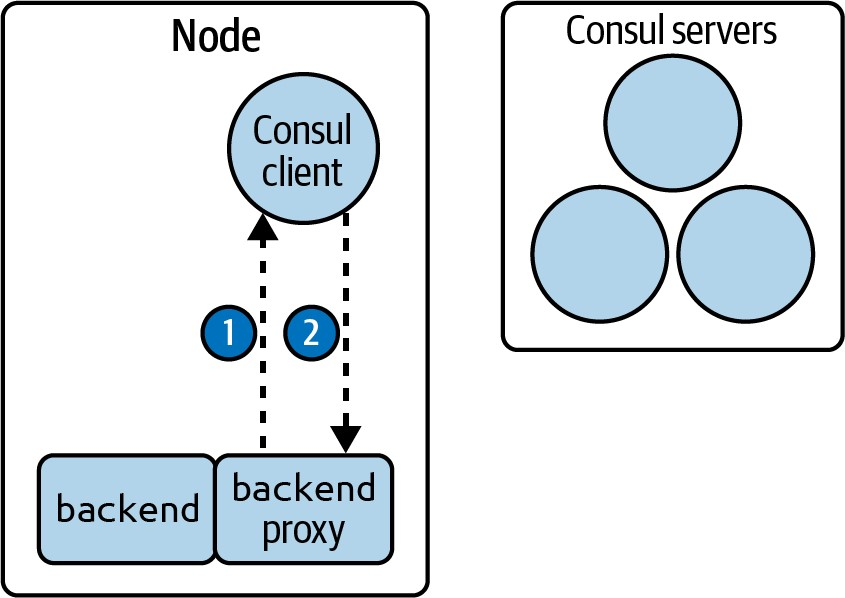
\includegraphics[width=0.7\linewidth]{Pics/example2}
		\caption{\label{fig:example2} Client Consul cấu hình proxy backend.}
		\label{fig:example2}
	\end{figure}
	
	\hspace{0.3cm}{Bây giờ hãy tưởng tượng rằng có một dịch vụ khác gọi là giao diện người dùng đang chạy trên một Node khác trong cụm và dịch vụ giao diện người dùng được cấu hình để giao tiếp với dịch vụ backend (hiển thị trong Hình 2.9).\\}
	
	\begin{figure}[h]
		\centering
		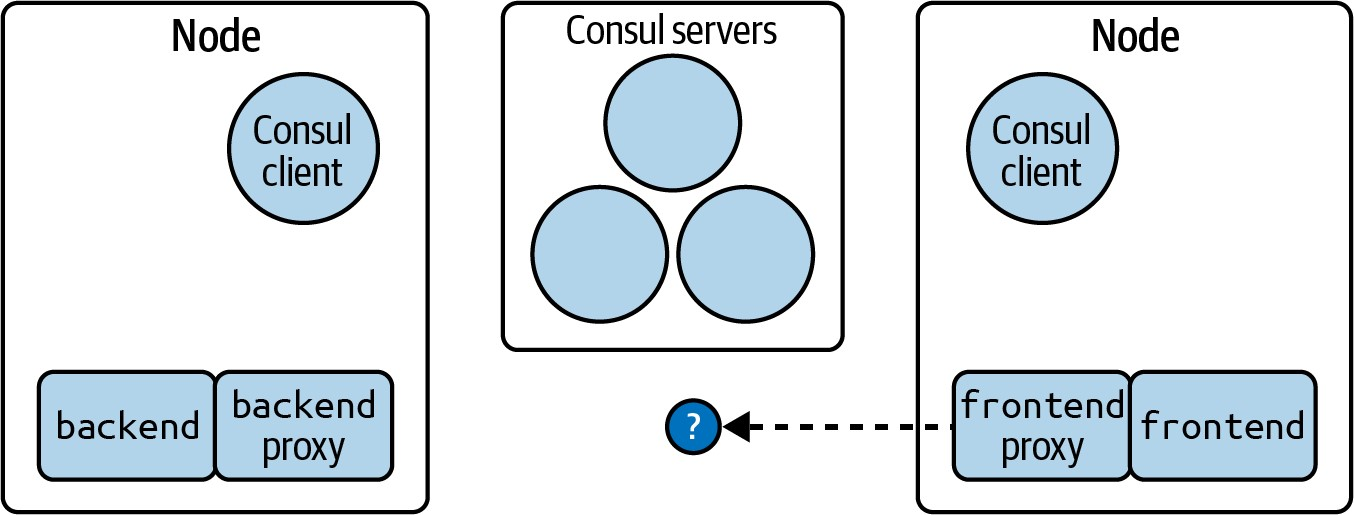
\includegraphics[width=0.7\linewidth]{Pics/example3}
		\caption{\label{fig:example3} Dịch vụ giao diện người dùng được cấu hình để nói chuyện với dịch vụ backend, nhưng nó chưa biết dùng địa chỉ nào.}
		\label{fig:example3}
	\end{figure}
	

	\begin{figure}[h]
		\centering
		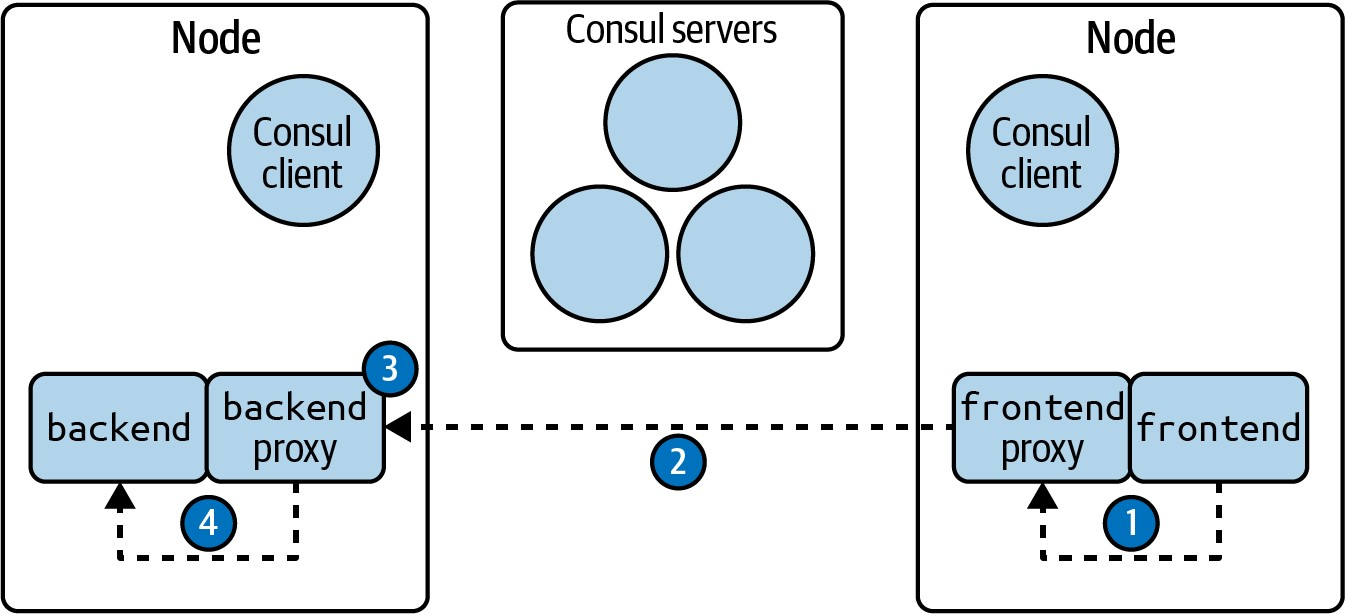
\includegraphics[width=0.7\linewidth]{Pics/example5}
		\caption{\label{fig:example5} Các proxy Sidecar ghi lại lưu lượng trong và ngoài và tuân theo các quy tắc được cấu hình của chúng để hành động trên lưu lượng đó.}
		\label{fig:example5}
	\end{figure}
	
	\hspace{0.3cm}{Ví dụ này minh họa cách máy chủ Consul, client và proxy sidecar hoạt động cùng nhau. Máy chủ Consul và client giao tiếp để chia sẻ dữ liệu về cụm và định cấu hình proxy sidecar. Các proxy Sidecar nắm bắt lưu lượng truy cập vào và ra và tuân theo các quy tắc được định cấu hình của chúng để hành động trên lưu lượng đó, chẳng hạn như bằng cách định tuyến nó tới một proxy khác hoặc không cho phép lưu lượng vì nó không được phép.}
	
	\subsection{Consul so với servece mesh khác}
	\hspace{1cm}{Có nhiều service mesh khác trên thị trường, chẳng hạn như Istio và Linkerd. Hầu hết các mắt service mesh đều tuân theo cùng một kiến trúc chung với một control plane quản lý các proxy sidecar. Consul là duy nhất trong số các mắt lưới khác ở chỗ control plane của nó có thể chạy hoàn toàn tách biệt với Kubernetes. Điều này có nghĩa là nếu chúng ta đang quản lý một cụm máy ảo thì chúng ta cũng không cần chạy Kubernetes.\\}
	
	\hspace{0.3cm}{Mỗi service mesh đều có ưu và nhược điểm tùy thuộc vào mục đích sử dụng chính xác của chúng ta. Một cách tiếp cận tốt để chọn service mesh là tập trung vào ba trường hợp sử dụng hàng đầu, chẳng hạn như bảo mật, khả năng quan sát và hỗ trợ đa cụm, sau đó kiểm tra các service mesh phổ biến nhất và chọn một lưới mà chúng ta cảm thấy phù hợp nhất.}
	
	\subsection{Các tính năng khác của Consul}
	\hspace{1cm}{Consul không chỉ là một mạng service mesh. Đây cũng là kho lưu trữ khóa/giá trị cho cấu hình dịch vụ và giải pháp khám phá dịch vụ DNS. Khi sử dụng DNS, không có proxy sidecar. Các yêu cầu được định tuyến trực tiếp giữa các dịch vụ. Điều này có nghĩa là không có tính năng mã hóa, quan sát hoặc kiểm soát lưu lượng tự động.\\}
	
	\section{Bảo mật trong Consul}
	\hspace{1cm}{Trong thế giới ngày nay, an ninh là tối quan trọng. Những kẻ tấn công tinh vi liên tục thăm dò các lỗ hổng có thể dẫn đến việc dữ liệu người dùng bị đánh cắp và hệ thống bị gián đoạn. Những cuộc tấn công này có thể hủy hoại danh tiếng của công ty và tiêu tốn hàng trăm nghìn đô la. Đồng thời, việc bảo vệ chống lại các cuộc tấn công này đang trở nên khó khăn hơn khi việc triển khai microservice ngày càng lớn và phức tạp hơn - do đó làm tăng mục tiêu tấn công của chúng.\\}
	
	\hspace{0.3cm}{Có nhiều khía cạnh để bảo mật hệ thống của tổ chức mặc dù service mesh không thể giải quyết tất cả các khía cạnh đó nhưng nó đóng một vai trò quan trọng. Service mesh thực hiện các cải tiến bảo mật thông qua proxy sidecar chặn tất cả lưu lượng truy cập vào và ra khỏi dịch vụ. Một service mesh có thể cung cấp:}
	
	\begin{itemize}
		\item Mã hóa lưu lượng giữa các dịch vụ.
		\item Thực thi các quy tắc về dịch vụ nào có thể giao tiếp với nhau và loại yêu cầu nào được phép - ví dụ: đường dẫn HTTP nào có thể được truy cập.
		\item Một số giảm thiểu chống lại các cuộc tấn công từ chối dịch vụ bằng cách tăng độ tin cậy của dịch vụ.
	\end{itemize}

	\hspace{0.3cm}{Tuy nhiên, vì nó hoạt động ở cấp độ nền tảng nên service mesh không thể cung cấp:}
	
	\begin{itemize}
		\item Tự động vá các thư viện dễ bị tấn công.
		\item Loại bỏ các lỗi bảo mật trong mã code dịch vụ.
		\item Xác thực và ủy quyền người dùng (ví dụ: xác thực mật khẩu).
		\item Phát hiện xâm nhập (Phát hiện xâm nhập đang giám sát hoạt động đáng ngờ. Consul có thể giúp phát hiện xâm nhập vì nó cung cấp số liệu về các yêu cầu bị từ chối. Nếu một dịch vụ đột nhiên có nhiều yêu cầu bị từ chối, có khả năng kẻ tấn công đang cố truy cập dịch vụ đó).
		\item Các cải tiến bảo mật cấp dịch vụ khác.
	\end{itemize}

	\hspace{0.3cm}{Các cải tiến bảo mật mà service mesh cung cấp - mã hóa lưu lượng giữa các dịch vụ và thực thi các quy tắc về dịch vụ nào có thể giao tiếp với nhau - là một phần của việc triển khai mô hình bảo mật được gọi là zero trust network.\\}
	
	\hspace{0.3cm}{Phần này bắt đầu với phần mô tả về mô hình zero trust network và lý do tại sao nó là một cải tiến so với mô hình cũ hơn. Sau đó, trình bày cách Consul triển khai zero trust network và mô tả mã hóa TLS.}
	\subsection{Zero trust network trong Consul}
	\hspace{1cm}{Kiến trúc an ninh mạng truyền thống là theo mô hình castle and moat. Trong mô hình castle and moat, các dịch vụ được triển khai trong một mạng riêng nội bộ (castle - lâu đài) không được kết nối với internet công cộng. Tường lửa (moat - hào nước) bảo vệ quyền truy cập vào mạng nội bộ (Tường lửa là phần mềm hoặc phần cứng kiểm soát quyền truy cập ở rìa mạng - nơi các hệ thống được kết nối với cả mạng riêng và mạng công cộng). Bộ cân bằng tải được triển khai bên ngoài mạng riêng và được phép truy cập thông qua tường lửa. Vì tường lửa đã được đặt sẵn, giả định rằng mọi thứ chạy bên trong mạng nội bộ đều có thể tin cậy được. Vì lý do này, không cần mã hóa, xác thực hoặc ủy quyền giữa các dịch vụ nội bộ.\\}
	
	\begin{figure}[h]
		\centering
		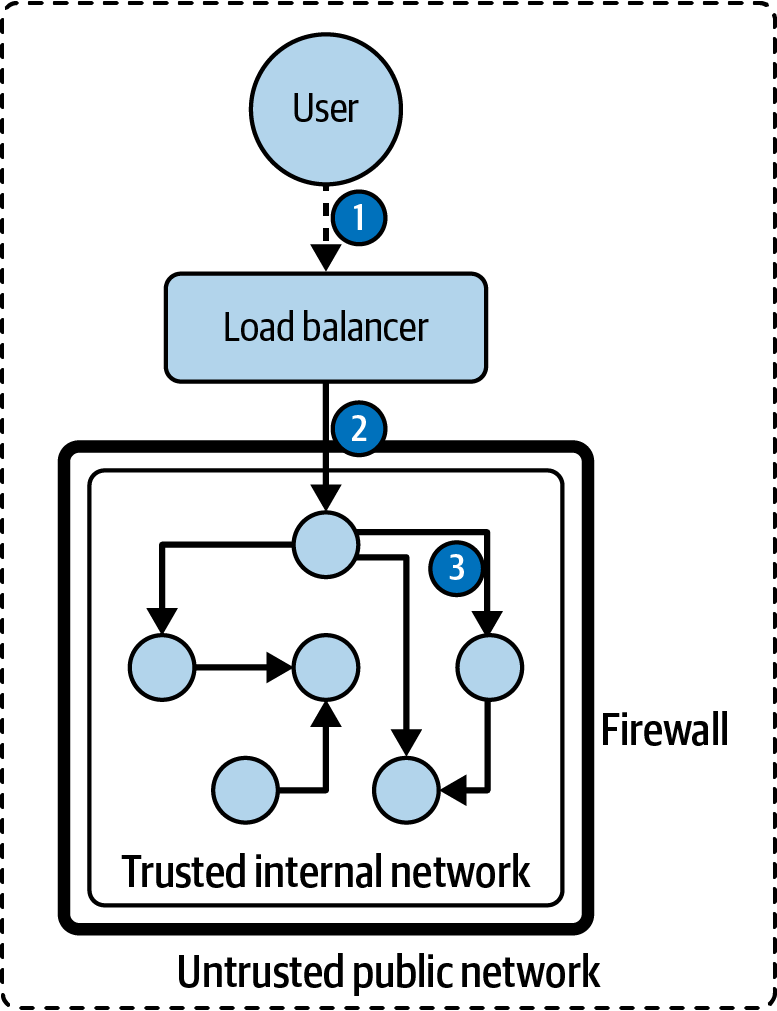
\includegraphics[width=0.5\linewidth]{Pics/castle_and_moat_modal}
		\caption{\label{fig:castleandmoatmodal} Định tuyến bên trong kiến trúc castle and moat.}
		\label{fig:castleandmoatmodal}
	\end{figure}
	
	\hspace{0.3cm}{Hình 2.13 cho thấy lưu lượng truy cập được định tuyến như thế nào qua kiến trúc castle and moat. Ở bước 1, yêu cầu của người dùng được chuyển đến bộ cân bằng tải. Bộ cân bằng tải chuyển tiếp yêu cầu qua tường lửa tới một dịch vụ đang chạy trong mạng nội bộ đáng tin cậy (bước 2). Dịch vụ đó thực hiện cuộc gọi đến các dịch vụ upstream của nó (bước 3). Các cuộc gọi này không được mã hóa và các dịch vụ upstream không kiểm tra ủy quyền vì các cuộc gọi đến từ bên trong mạng nội bộ đáng tin cậy.\\}
	
	\hspace{0.3cm}{Vấn đề với mô hình castle and moat là những kẻ tấn công giành được quyền truy cập vào toàn bộ hệ thống nếu chúng xâm phạm bất kỳ điểm nào trong mạng nội bộ. Điều này có nghĩa là bảo mật của hệ thống chỉ tốt bằng liên kết yếu nhất của nó.\\}
	
	\begin{figure}[h]
		\centering
		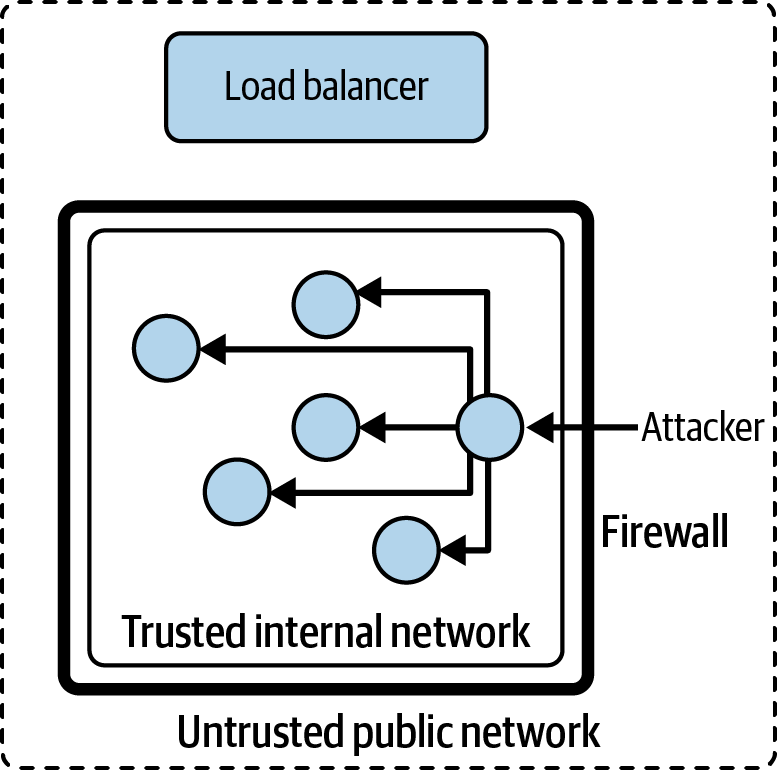
\includegraphics[width=0.5\linewidth]{Pics/threat_of_castle_and_moat}
		\caption{\label{fig:threatofcastleandmoat} Trong kiến trúc castle and moat, nếu kẻ tấn công xâm phạm một dịch vụ, chúng có thể yêu cầu tất cả các dịch vụ và cơ sở dữ liệu bên trong mạng.}
		\label{fig:threatofcastleandmoat}
	\end{figure}
	
	\hspace{0.3cm}{Đây không phải là một điểm yếu lý thuyết. Vào năm 2015, tin tặc đã đánh cắp hàng triệu hồ sơ nhạy cảm về nhân viên chính phủ từ Văn phòng Quản lý Nhân sự Hoa Kỳ (OPM). Những kẻ tấn công đã giành được quyền truy cập bằng cách xâm nhập vào hệ thống của một công ty hợp đồng có máy chủ có toàn quyền truy cập vào mạng OPM. Từ đó, họ có thể tự do trích xuất dữ liệu từ các máy chủ OPM.\\}
	
	\hspace{0.3cm}{Điểm yếu của hệ thống castle and moat là không thể chấp nhận được đối với hầu hết các công ty, vì vậy các kỹ sư bảo mật đề xuất một mô hình khác: zero trust network.\\}
	
	\hspace{0.3cm}{Trong zero trust network, chúng ta cho rằng mạng nội bộ bị xâm phạm. Do đó, các dịch vụ không hoàn toàn tin tưởng các yêu cầu đơn giản chỉ vì chúng đến từ bên trong mạng nội bộ. Thay vào đó, các dịch vụ thực hiện mã hóa, xác thực và ủy quyền cho tất cả các yêu cầu.}
	
	\subsubsection{Mã hóa}
	\hspace{1cm}{Quá trình sửa đổi dữ liệu sao cho bên thứ ba không thể đọc dữ liệu gốc chưa sửa đổi, nhưng người nhận thì có thể. Trong mạng máy tính, quy trình mã hóa TLS thường được sử dụng để đảm bảo rằng các bên thứ ba không thể chặn và đọc dữ liệu được gửi giữa người dùng và trang web mà họ đang xem. TLS được sử dụng bí mật khi người dùng truy cập các trang web https://.}
	
	\subsubsection{Xác thực}
	\hspace{1cm}{Quá trình xác thực rằng một thực thể là người đã được xác minh, công nhận. Ví dụ: nếu người dùng tuyên bố là người dùng quản trị, thì xác thực là quá trình kiểm tra xem mật khẩu họ cung cấp có khớp với mật khẩu dự kiến hay không. Sau khi một thực thể được xác thực, chúng ta vẫn cần kiểm tra xem họ có được phép thực hiện hành động mà họ đang cố thực hiện hay không.}
	
	\subsubsection{Ủy quyền}
	\hspace{1cm}{Quá trình xác thực rằng một thực thể được xác thực được phép thực hiện một hành động cụ thể nào đó hay không. Ví dụ: người dùng đã đăng nhập có thể được xác thực nhưng có lẽ họ không được phép xem bảng quản trị.}

	\subsection{Mã hóa trong Consul}
	\hspace{1cm}{Mã hóa là cần thiết trong mạng zero trust network vì dịch vụ bị xâm phạm có thể đọc lưu lượng được truyền giữa các dịch vụ khác- điều này được gọi là traffic sniffng hoặc tấn công trung gian. (Có nhiều cơ chế để một dịch vụ bị xâm nhập chặn bắt lưu lượng truy cập. Nếu dịch vụ bị xâm nhập nằm trên cùng một node với một dịch vụ khác, dịch vụ đó có thể có quyền kiểm tra lưu lượng mạng của các quy trình khác. Hoặc một dịch vụ bị xâm phạm có thể sử dụng một kỹ thuật gọi là giả mạo Giao thức phân giải địa chỉ (ARP) để khiến một dịch vụ khác gửi nhầm lưu lượng truy cập của nó đến dịch vụ bị xâm phạm thay vì đích dự kiến).\\}
	\newpage
	\begin{figure}[h]
		\centering
		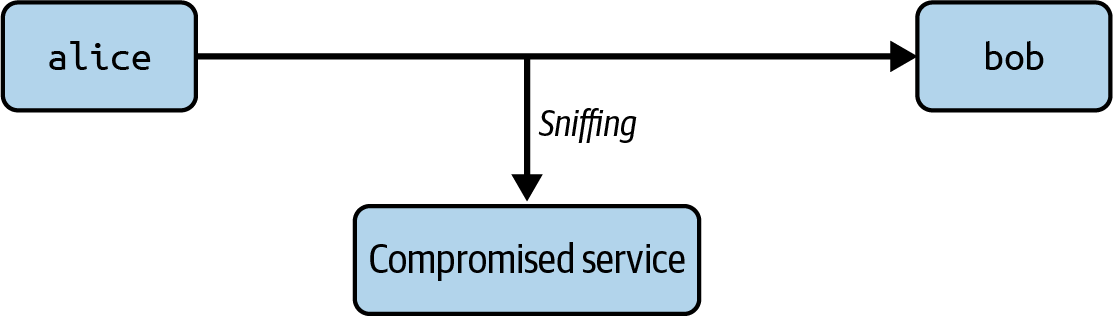
\includegraphics[width=0.7\linewidth]{Pics/sniffing}
		\caption{\label{fig:sniffing} Một dịch vụ bị xâm nhập có thể chặn truy tìm được gửi giữa hai dịch vụ khác.}
		\label{fig:sniffing}
	\end{figure}
	
	\hspace{0.3cm}{Mã hóa ngăn chặn các cuộc tấn công trung gian vì những kẻ tấn công không thể đọc dữ liệu được gửi giữa hai dịch vụ. Chỉ dịch vụ đích mới có thể giải mã dữ liệu. Như thể hiện trong hình, nếu Bob là dịch vụ duy nhất có khả năng giải mã lưu lượng truy cập từ dịch vụ Alice, thì việc kẻ tấn công chặn lưu lượng cũng không thành vấn đề.\\}
	
	\begin{figure}[h]
		\centering
		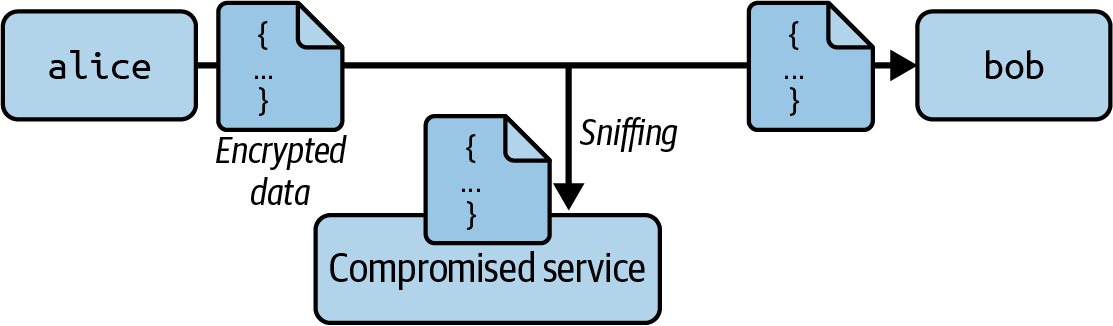
\includegraphics[width=0.7\linewidth]{Pics/encrypt_prevent_sniffing}
		\caption{\label{fig:encryptpreventsniffing} Dữ liệu điện tử hiện đã được mã hóa, do đó, ngay cả khi dịch vụ bị xâm phạm sniffing, chúng cũng không thể lấy được nội dung gốc.}
		\label{fig:encryptpreventsniffing}
	\end{figure}
	
	\hspace{0.3cm}{Consul sử dụng mã hóa TLS để mã hóa lưu lượng giữa các dịch vụ.}
	
	\subsubsection{Mã hóa TLS}
	\hspace{1cm}{Mã hóa TLS có ba bước (xem Hình 2.16 để biết minh họa):}
	\begin{enumerate}
	\item Dịch vụ nguồn và đích đồng ý về khóa mã hóa.
	\item Dịch vụ nguồn mã hóa tin nhắn của nó bằng khóa đã thỏa thuận và gửi tin nhắn được mã hóa đến dịch vụ đích.
	\item Dịch vụ đích giải mã tin nhắn bằng khóa đã thỏa thuận.
	\end{enumerate}

	\begin{figure}[h]
		\centering
		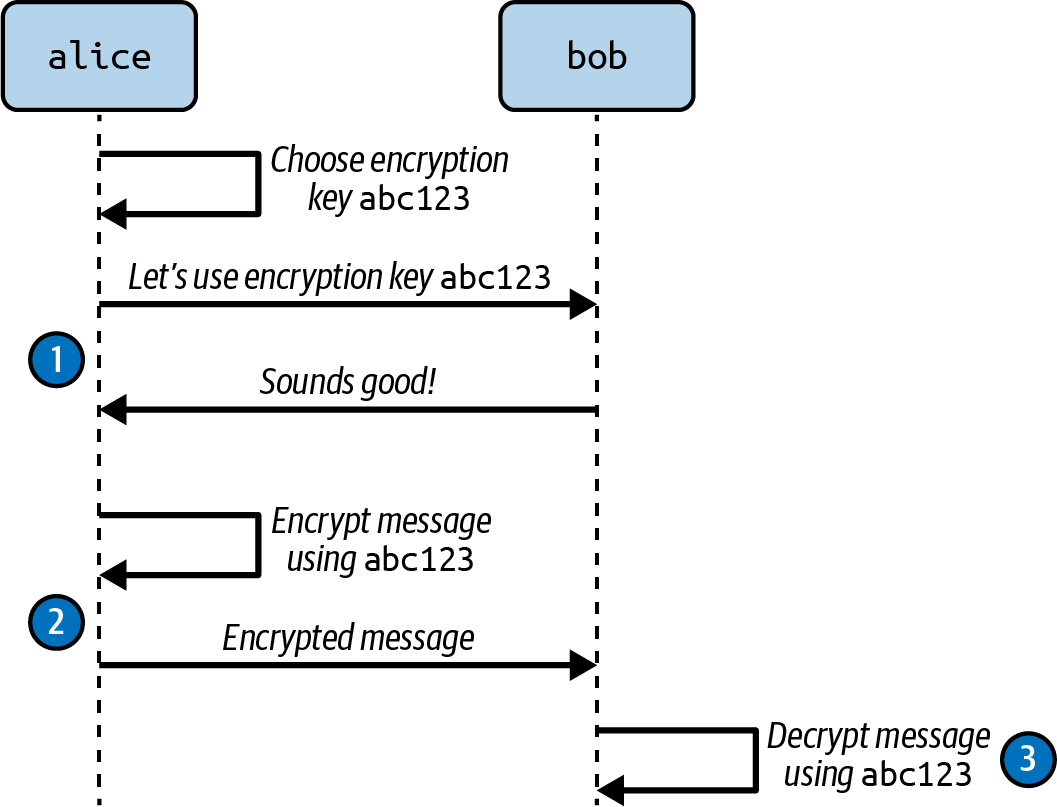
\includegraphics[width=0.7\linewidth]{Pics/TLS}
		\caption{\label{fig:tls} Một minh họa về mã hóa TLS.}
		\label{fig:tls}
	\end{figure}
	
	\hspace{0.3cm}{Miễn là những kẻ tấn công trung gian không biết khóa mã hóa, chúng không thể giải mã tin nhắn. Loại mã hóa này được gọi là mã hóa đối xứng vì cả hai bên đều biết khóa mã hóa.\\}
	
	\hspace{0.3cm}{Nhưng làm thế nào để khóa mã hóa đối xứng được thỏa thuận mà không có kẻ tấn công chặn nó? Đây là lúc mật mã khóa công khai phát huy tác dụng.\\}
	
	\hspace{0.3cm}{Mật mã khóa công khai là một phương pháp mã hóa sử dụng các cặp khóa: khóa bí mật và khóa công khai. Các khóa được liên kết về mặt toán học sao cho các thông báo được mã hóa bằng khóa công khai chỉ có thể được giải mã bằng khóa bí mật. Mật mã khóa công khai cho phép cả hai dịch vụ đồng ý với khóa mã hóa đối xứng mà khóa đó không được gửi qua mạng, nơi khóa có thể bị đánh cắp.\\}
	
	\hspace{0.3cm}{Hãy xem qua một ví dụ sử dụng hai dịch vụ tưởng tượng, Alice và Bob, muốn đồng ý về một khóa mã hóa đối xứng:}
	
	\begin{enumerate}
	\item Dịch vụ Alice tạo hai khóa, một khóa bí mật có tên alice-priv và một khóa công khai có tên alice-pub.
	\item Dịch vụ Alice gửi khóa công khai của nó - alice-pub đến dịch vụ Bob. Khóa được gửi dưới dạng văn bản rõ để kẻ tấn công có thể nhìn thấy khóa.
	\item Dịch vụ Bob cũng làm như vậy. Nó tạo ra hai khóa, bob-priv và bob-pub, đồng thời gửi khóa bob-pub cho Alice. Một lần nữa, kẻ tấn công có thể thấy khóa bob-pub.
	\item Ngay bây giờ Alice sẵn sàng gửi khóa mã hóa đối xứng cho Bob. Alice mã hóa khóa mã hóa đối xứng bằng khóa công khai của Bob - bob-pub.
	\item Alice gửi thông điệp được mã hóa này cho Bob. Một lần nữa, kẻ tấn công có thể nhìn thấy thông điệp được mã hóa này, nhưng điều kỳ diệu của mật mã khóa công khai là kẻ tấn công không thể giải mã thông điệp bằng các khóa công khai alice-pub hoặc bob-pub. Thuật toán sử dụng để mã hóa thông điệp được thiết kế sao cho chỉ khóa bí mật của Bob (bob-priv) mới có thể giải mã nó.
	\item Bob nhận được thông điệp được mã hóa và sử dụng khóa riêng của nó - bob-priv để giải mã.
	\item Giờ đây, khóa mã hóa đối xứng đã được thỏa thuận một cách an toàn, Alice và Bob có thể tự do gửi thêm thông điệp bằng cách mã hóa chúng khóa mã hóa đối xứng.
	\end{enumerate}

	\begin{figure}[h]
		\centering
		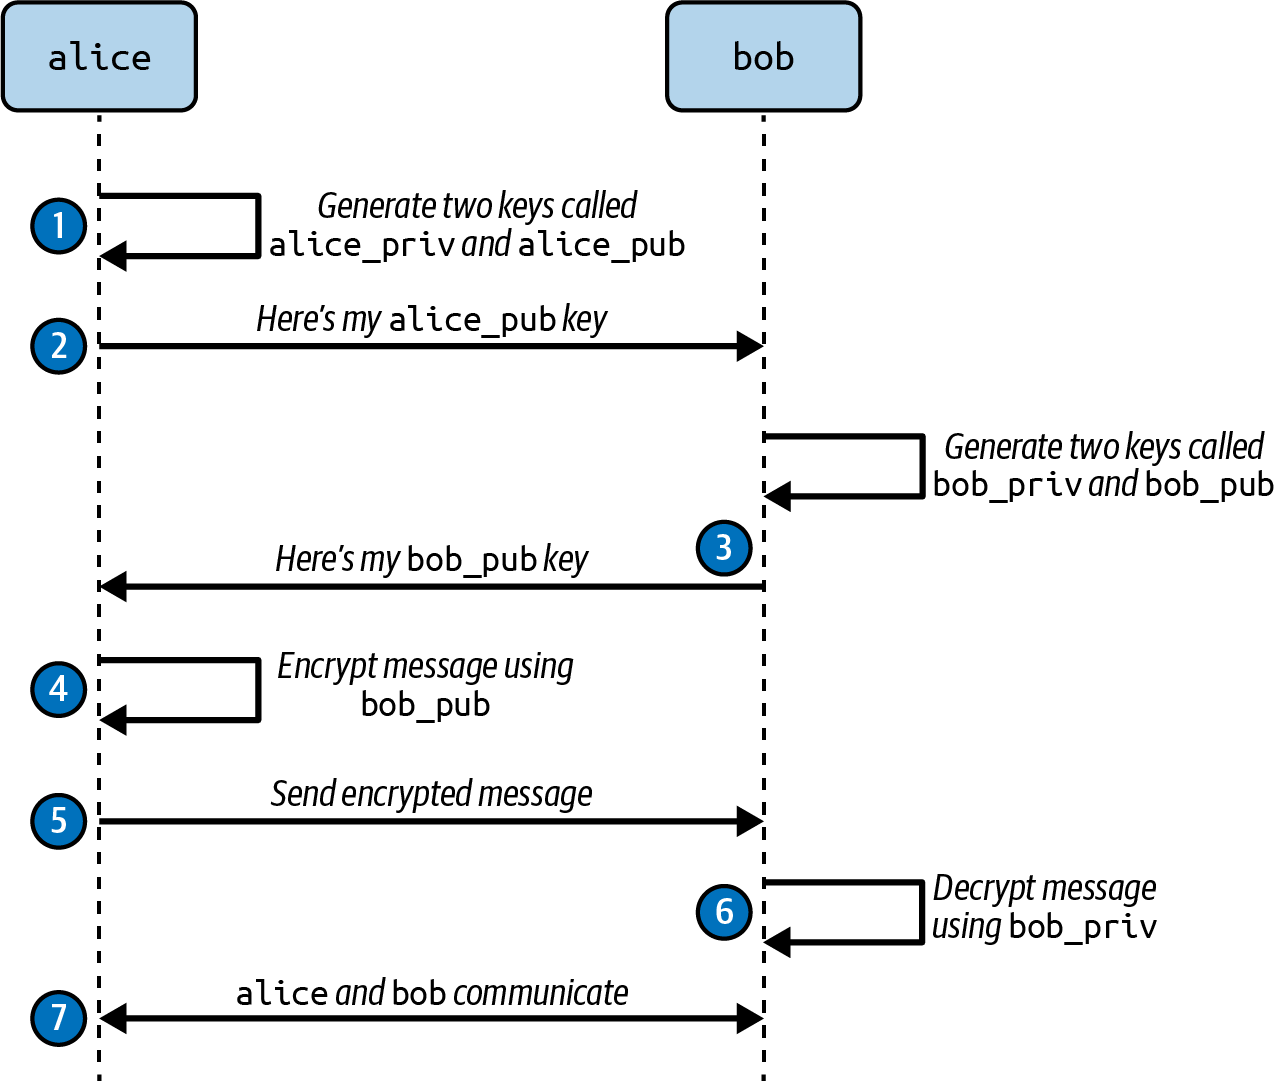
\includegraphics[width=0.7\linewidth]{Pics/public-key_cryptography}
		\caption{\label{fig:public-keycryptography} Sơ đồ mật mã khóa công khai.}
		\label{fig:public-keycryptography}
	\end{figure}
	
	\hspace{0.3cm}{Vì lý do hiệu suất, mật mã khóa công khai chỉ được sử dụng khi bắt đầu kết nối TLS để đồng ý một cách an toàn về khóa mã hóa đối xứng. Từ đó trở đi, khóa mã hóa đối xứng đó được sử dụng để mã hóa tất cả dữ liệu được gửi giữa hai dịch vụ.\\}
	
	\hspace{0.3cm}{Đó chính là cách hoạt động của mã hóa TLS, Consul sử dụng TLS để mã hóa lưu lượng service mesh.}
	\newpage
	\subsubsection{Mã hóa trong Consul}
	\hspace{1cm}{Mã hóa TLS trong Consul được bật theo mặc định. Khi một dịch vụ đưa ra yêu cầu thông qua proxy sidecar của nó, proxy sẽ tự động mã hóa yêu cầu đó bằng TLS. Dịch vụ có thể tiếp tục thực hiện các yêu cầu không được mã hóa và proxy đảm bảo các yêu cầu đó được mã hóa trước khi chúng rời khỏi mạng cục bộ.\\}
	
	\hspace{0.3cm}{Quá trình này được thể hiện trong hình bên dưới. Ở bước 1, Consul cung cấp khóa công khai và khóa bí mật cho từng proxy. Khi giao diện người dùng gửi một yêu cầu không được mã hóa đến chương trình backend, thì yêu cầu đó sẽ bị chặn bởi proxy của giao diện người dùng (bước 2) và mã hóa yêu cầu đó trước khi chuyển tiếp đến chương trình backend (bước 3). Ở phía bên nhận, proxy của chương trình backend sẽ chặn yêu cầu (bước 4) và giải mã nó trước khi chuyển tiếp đến dịch vụ đích (bước 5).\\}
	
	\begin{figure}[h]
		\centering
		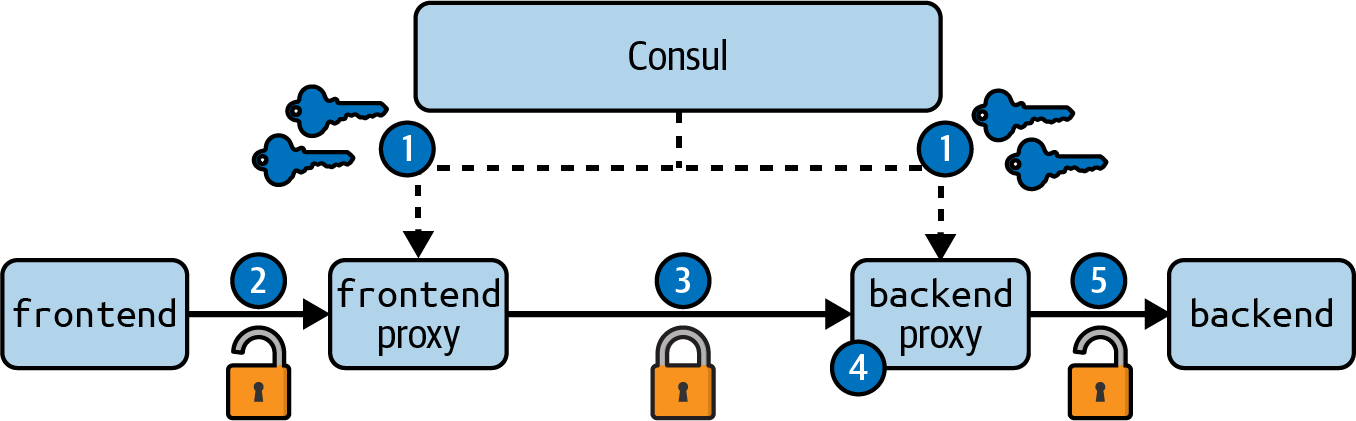
\includegraphics[width=0.7\linewidth]{Pics/Sidecar_proxies_automatically_encrypt}
		\caption{\label{fig:sidecarproxiesautomaticallyencrypt} Sidecar proxy tự động mã hóa lưu lượng bằng TLS.}
		\label{fig:sidecarproxiesautomaticallyencrypt}
	\end{figure}
	
	\hspace{0.3cm}{Với cơ chế này, các dịch vụ không cần phải sửa đổi để sử dụng TLS - tất cả đều diễn ra tự động mà chúng không hề hay biết.\\}
	
	\hspace{0.3cm}{Đó chính xác là cách Consul thực hiện mã hóa. Mã hóa là điều cần thiết trong một zero trust network, nhưng nó vẫn không đủ. Nếu không có xác thực và ủy quyền, một dịch vụ bị xâm phạm vẫn có thể thực hiện các yêu cầu thông qua proxy sidecar của nó tới bất kỳ dịch vụ nào trong mạng.}
	
	\subsection{Xác thực trong Consul}
	\hspace{1cm}{Xác thực là quá trình xác minh rằng ai đó là người mà đã được xác minh; đó là về việc xác minh danh tính. Trong mạng dịch vụ, điều này có hai phần: dịch vụ nguồn phải xác minh rằng dịch vụ đích thực sự là dịch vụ mà nó muốn giao tiếp và dịch vụ đích phải xác minh rằng dịch vụ nguồn thực sự là dịch vụ mà nó yêu cầu.\\}
	
	\hspace{0.3cm}{Cụ thể, nếu giao diện người dùng đang gọi phần backend, thì giao diện người dùng cần đảm bảo rằng nó thực sự đang nói chuyện với phần backend. Nếu nó không kiểm tra, thì nó có thể đang gửi yêu cầu của mình tới kẻ tấn công. Backend cũng cần xác minh dịch vụ nào đang thực hiện yêu cầu để có thể kiểm tra xem dịch vụ đó có được phép giao tiếp với nó hay không.\\}
	
	\hspace{0.3cm}{Consul cũng tận dụng TLS để thực hiện xác thực. Khi các dịch vụ trao đổi khóa công khai của họ, họ thực sự trao đổi chứng chỉ. Chứng chỉ này chứa khóa công khai và thông tin về dịch vụ, chẳng hạn như ID của nó.\\}
	
	\hspace{0.3cm}{Đây là các bước liên quan đến xác thực TLS:}
	
	\begin{enumerate}
	\item Consul cấp chứng chỉ công khai và khóa bí mật cho từng dịch vụ. Được mã hóa trong chứng chỉ công khai là ID của dịch vụ đó.
	\item Trong quá trình trao đổi khóa, chứng chỉ công khai cho mỗi dịch vụ được trao đổi.
	\item Mỗi dịch vụ kiểm tra chứng chỉ công khai của dịch vụ kia và đảm bảo rằng ID dịch vụ là những gì được mong đợi. Ví dụ: dịch vụ giao diện người dùng sẽ xác minh rằng chứng chỉ dành cho dịch vụ backend và dịch vụ backend sẽ xác minh rằng chứng chỉ dành cho dịch vụ giao diện người dùng.
	\item Nếu danh tính được xác minh, yêu cầu sẽ tiếp tục.
	\end{enumerate}

	\begin{figure}[h]
		\centering
		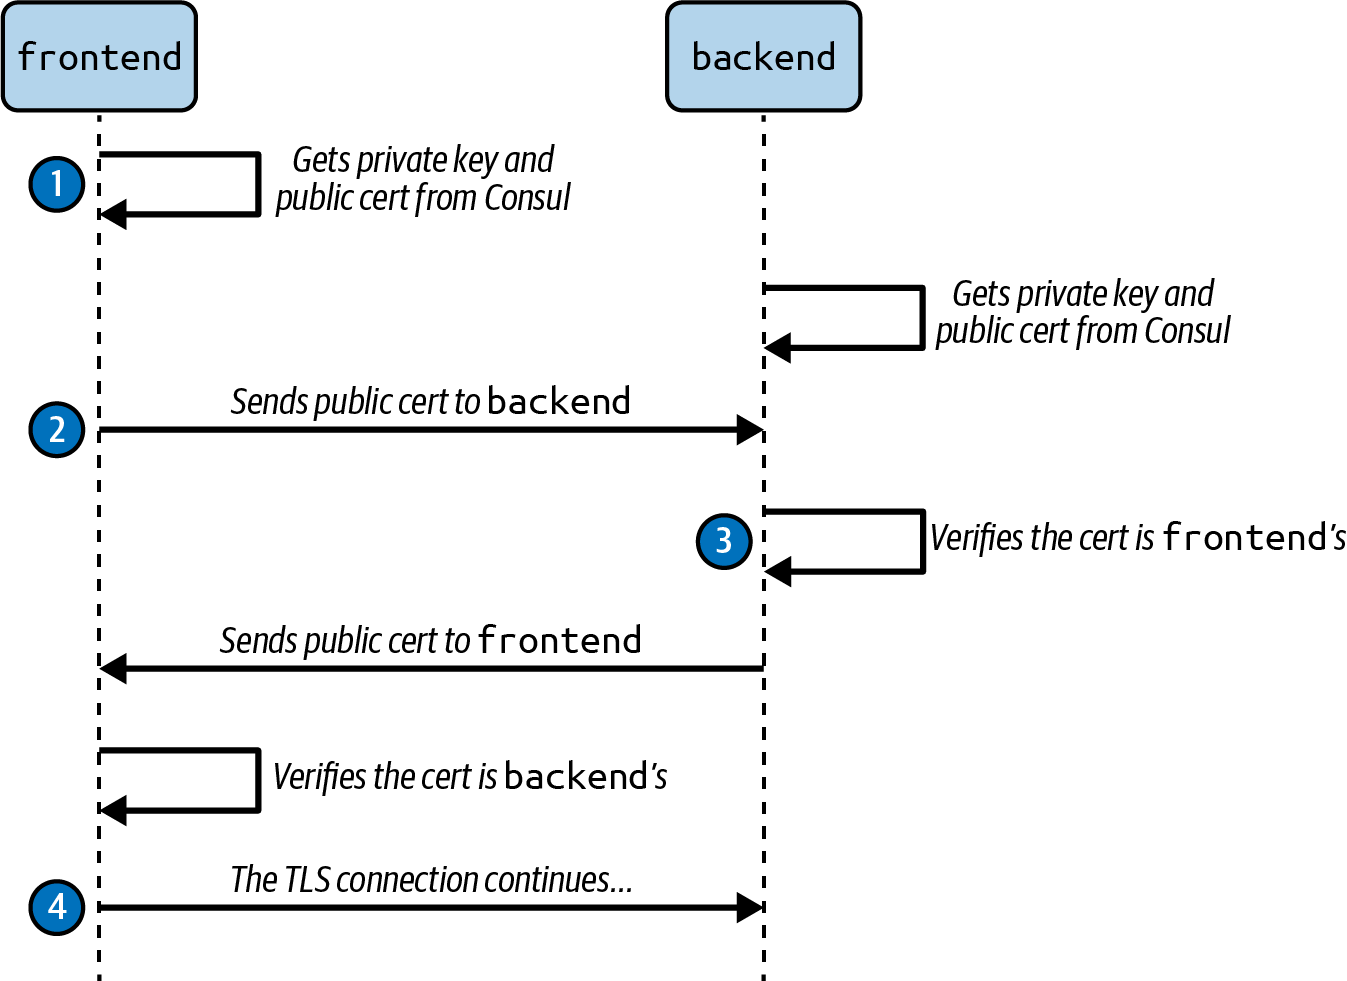
\includegraphics[width=0.7\linewidth]{Pics/TLS_provide_authentication}
		\caption{\label{fig:tlsprovideauthentication} TLS được sử dụng để cung cấp xác thực.}
		\label{fig:tlsprovideauthentication}
	\end{figure}
	
	\hspace{0.3cm}{Chúng ta có thể tự hỏi điều gì ngăn kẻ tấn công tạo chứng chỉ công khai của riêng chúng để mạo danh bất kỳ dịch vụ nào. Để ngăn chặn điều này, Consul hoạt động như một cơ quan cấp chứng chỉ.\\}
	
	\hspace{0.3cm}{Cơ quan cấp chứng chỉ là một thực thể cấp chứng chỉ được ký bằng mật mã sao cho chúng chỉ có thể đến từ cơ quan cấp chứng chỉ đó. Cơ quan cấp chứng chỉ cũng có chứng chỉ công khai được gọi là chứng chỉ của cơ quan cấp chứng chỉ (chứng chỉ CA). Khi xuất trình chứng chỉ công khai của dịch vụ - ví dụ: chứng chỉ backend - bên thứ ba có thể sử dụng chứng chỉ CA để kiểm tra xem chứng chỉ công khai có được ký bởi cơ quan cấp chứng chỉ đó hay không.\\}
	
	\hspace{0.3cm}{Cụ thể, ngoài chứng chỉ công khai và khóa bí mật mà Consul cấp cho từng dịch vụ, Consul còn cấp cho từng dịch vụ chứng chỉ CA của mình. Sau đó, chứng chỉ CA này có thể được sử dụng để xác minh rằng Consul thực sự đã cấp chứng chỉ công khai và việc tin cậy ID dịch vụ được mã hóa bên trong là an toàn.\\}
	
	\begin{figure}[h]
		\centering
		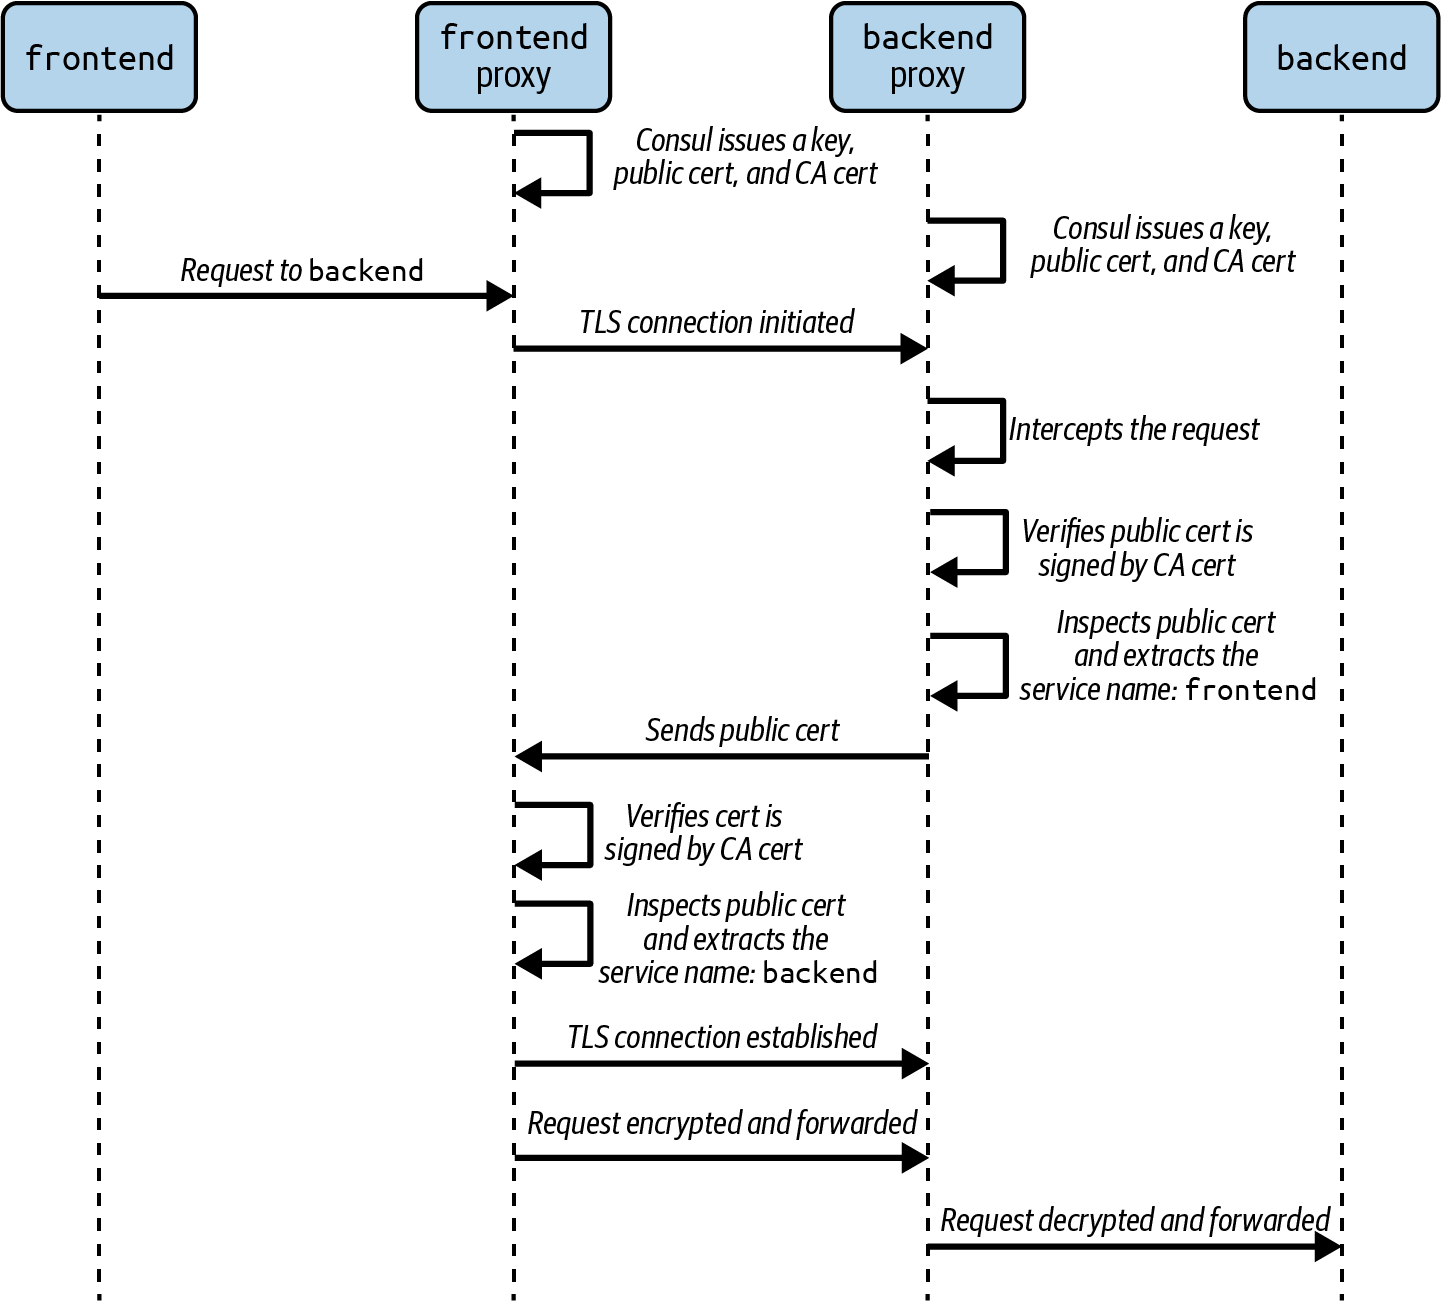
\includegraphics[width=0.7\linewidth]{Pics/frontend_talk_to_backend_securely}
		\caption{\label{fig:frontendtalktobackendsecurely} Quy trình khi giao diện người dùng giao tiếp với phần backend một cách an toàn.}
		\label{fig:frontendtalktobackendsecurely}
	\end{figure}
	
	\hspace{0.3cm}{Chúng ta có thể xem các chứng chỉ công khai của từng dịch vụ bằng công cụ openssl.}
	\subsection{Ủy quyền trong Consul}
	\hspace{1cm}{Ủy quyền là quá trình xác định xem một thực thể được xác thực có được phép thực hiện một hành động nhất định hay không. Ví dụ: dịch vụ này có được phép thực hiện các yêu cầu đối với dịch vụ đó hay được phép truy cập vào một đường dẫn HTTP cụ thể không?\\}
	
	\hspace{0.3cm}{Consul thực hiện ủy quyền thông qua hệ thống chủ đích của nó. Chủ đích là các quy tắc chi phối các dịch vụ nào được phép giao tiếp.\\}
	
	\hspace{0.3cm}{Mọi chủ đích đều có nguồn gốc và đích đến. Ví dụ: một chủ đích có thể cho phép một giao diện người dùng dịch vụ cụ thể (nguồn) kết nối với một dịch vụ backend cụ thể (đích). Ngoài ra, ký tự đại diện có thể được sử dụng làm nguồn hoặc đích, chẳng hạn như cho phép một cổng vào kết nối với bất kỳ dịch vụ nào hoặc bất kỳ dịch vụ nào kết nối với bất kỳ dịch vụ nào khác.\\}
	
	\hspace{0.3cm}{Ngoài việc chỉ định các quy tắc dựa trên dịch vụ nguồn và đích, chúng ta có thể sử dụng các chủ đích để kiểm soát các phương thức, đường dẫn và tiêu đề HTTP hoặc gRPC nào được ủy quyền. Consul gọi những chủ đích này là nhận biết ứng dụng vì chúng liên quan đến cách ứng dụng thực sự hoạt động. Ví dụ: bạn có thể tạo một chủ đích cho phép cổng vào truy cập vào bất kỳ đường dẫn nào trên dịch vụ giao diện người dùng ngoại trừ /admin.\\}
	
	\hspace{0.3cm}{Cơ chế thực thi chủ đích như sau:}
	
	\begin{enumerate}
	\item Dịch vụ nguồn gửi yêu cầu đến dịch vụ đích.
	\item Proxy của dịch vụ đích xác minh chứng chỉ công khai của dịch vụ nguồn và trích xuất tên dịch vụ từ ID.
	\item Proxy của dịch vụ đích kiểm tra danh sách các chủ đích của nó để đảm bảo rằng dịch vụ nguồn được phép thực hiện kết nối.
	\item Nếu đã đặt chủ đích nhận biết ứng dụng, proxy của dịch vụ đích cũng xác minh rằng yêu cầu cụ thể đó được cho phép.
	\end{enumerate}

	\hspace{0.3cm}{Proxy của giao diện người dùng cần biết địa chỉ của dịch vụ backend để thực hiện yêu cầu. Để thực hiện điều này, ứng dụng client Consul trên cùng một nút với dịch vụ giao diện người dùng sẽ xem danh mục máy chủ Consul để biết các phiên bản mới của dịch vụ backend (bước 1 trong Hình 2.10). Khi một phiên bản mới của dịch vụ backend được đăng ký vào danh mục, máy chủ Consul sẽ gửi địa chỉ mới đến ứng dụng client Consul (bước 2). Sau đó, máy client Consul cập nhật cấu hình proxy của dịch vụ giao diện người dùng với địa chỉ mới cho dịch vụ backend (bước 3).\\}
	\newpage
	\begin{figure}[h]
		\centering
		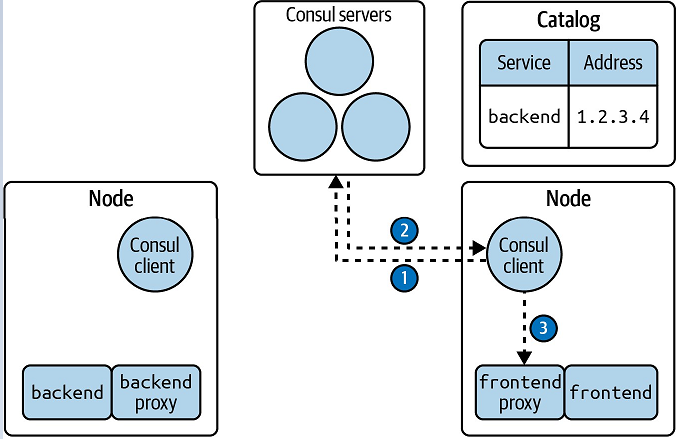
\includegraphics[width=0.7\linewidth]{Pics/example4}
		\caption{\label{fig:example4} Proxy của giao diện người dùng học địa chỉ của dịch vụ backend để thực hiện yêu cầu.}
		\label{fig:example4}
	\end{figure}
	
	\hspace{0.3cm}{Bây giờ proxy của dịch vụ giao diện người dùng biết địa chỉ của dịch vụ backend. Khi dịch vụ giao diện người dùng đưa ra yêu cầu của nó, proxy của giao diện người dùng sẽ chặn nó (bước 1). Proxy thấy rằng yêu cầu bị ràng buộc đối với dịch vụ backend và vì nó biết địa chỉ của dịch vụ backend, 1.2.3.4, nên nó sẽ chuyển tiếp yêu cầu đến địa chỉ đó (bước 2). Yêu cầu đến dịch vụ backend, nơi proxy của dịch vụ backend chặn nó (bước 3). Giả sử rằng proxy của backend được định cấu hình để chỉ cho phép các yêu cầu từ dịch vụ giao diện người dùng. Proxy kiểm tra yêu cầu và thấy rằng đó là từ dịch vụ giao diện người dùng, và do đó, nó cho phép yêu cầu thông qua (bước 4).\\}
	
	\begin{figure}[h]
		\centering
		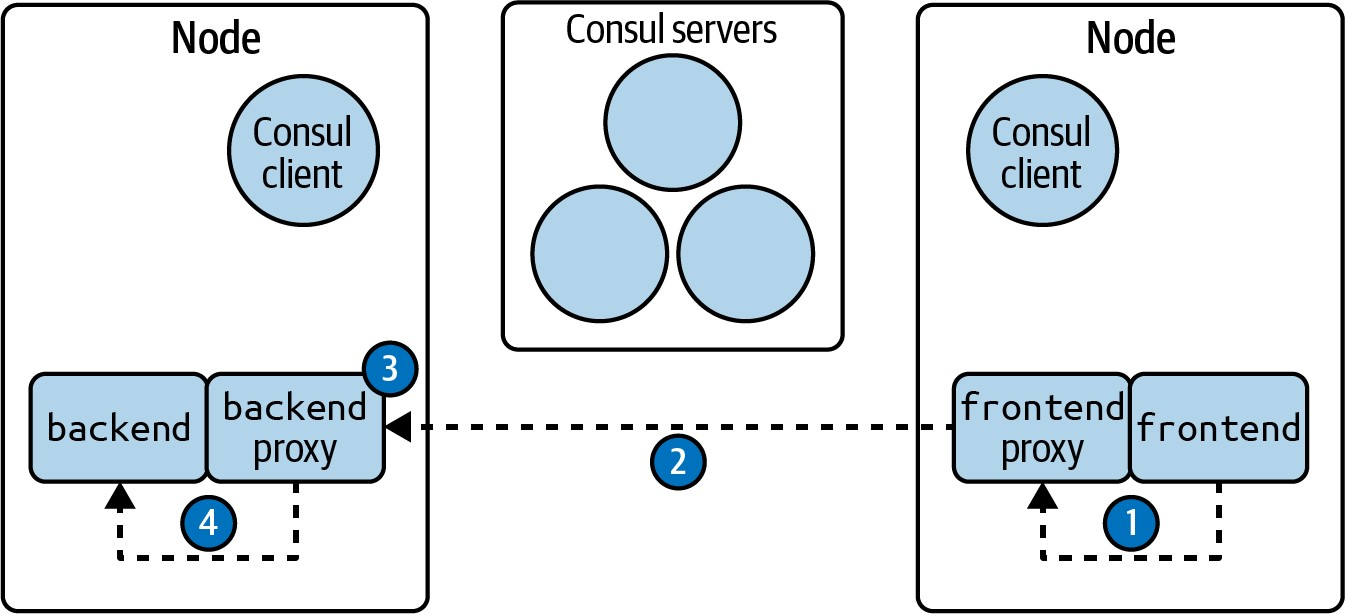
\includegraphics[width=0.7\linewidth]{Pics/example5}
		\caption{\label{fig:example5} Các proxy Sidecar ghi lại lưu lượng trong và ngoài và tuân theo các quy tắc được cấu hình của chúng để hành động trên lưu lượng đó.}
		\label{fig:example5}
	\end{figure}
	
	\hspace{0.3cm}{Ví dụ này minh họa cách máy chủ Consul, client và proxy sidecar hoạt động cùng nhau. Máy chủ Consul và client giao tiếp để chia sẻ dữ liệu về cụm và định cấu hình proxy sidecar. Các proxy Sidecar nắm bắt lưu lượng truy cập vào và ra và tuân theo các quy tắc được định cấu hình của chúng để hành động trên lưu lượng đó, chẳng hạn như bằng cách định tuyến nó tới một proxy khác hoặc không cho phép lưu lượng vì nó không được phép.}
	\newpage
	\section*{Kết luận chương 2}
	\addcontentsline{toc}{section}{Kết luận chương 2}
	\hspace{1.0cm}{Qua chương hai, chúng ta đã tìm hiểu về Service Mesh là gì, cách thức hoạt động của Service Mesh. Giới thiệu về Consul và khả năng bảo mật của Consul bên trong kubernetes. Tiếp theo, để tìm hiểu về khả năng bảo mật của Consul, chúng ta sẽ bắt đầu đến với chương 3, thực nghiệm. Ở chương tiếp theo, chúng ta sẽ có những phần thực nghiệm về Consul trong Kubernetes giúp chúng ta hiểu rõ hơn về Consul và cách Consul có thể bảo mật cho các Microservice bên trong Kubernetes.}
	\chapter{Triển khai Consul trên cụm Kubernetes}
	\section{Mô hình thực nghiệm}
	\begin{figure}[h]
	\centering
	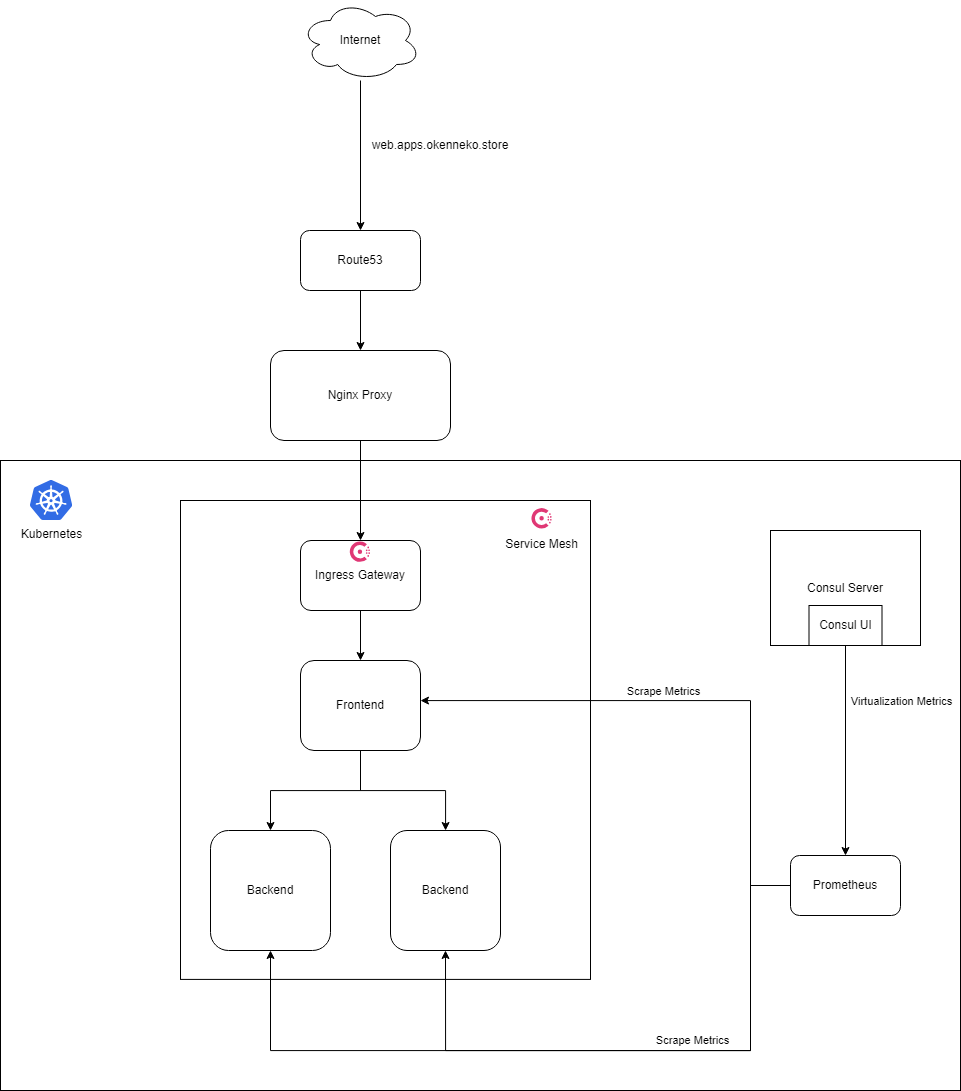
\includegraphics[width=0.7\linewidth]{Pics/diagram.drawio.png}
	\caption{\label{fig:diagram} Mô hình triển khai.}
	\label{fig:diagram}
	\end{figure}
	\section{Các bước triển khai Consul trên Kubernetes}
	\hspace{1.0cm}{Để triển khai Consul trên Kubernetes, chúng ta sẽ cần phải có những công cụ sau đây:\\}
	\begin{itemize}
		\item kubectl
		\item helm
		\item k9s
	\end{itemize}
	\hspace{0.3cm}{Dưới đây là các câu lệnh để triển khai Consul, chúng ta sẽ sử dụng Chart của Hashicorp cung cấp. Đầu tiên, chúng ta cần phải thêm nguồn chart vào trong dữ liệu Helm của chúng ta với câu lệnh sau:}
	\begin{lstlisting}[language=Bash]
	helm repo add hashicorp https://helm.releases.hashicorp.com
	\end{lstlisting}
	\hspace{1.0cm}{Tiếp theo, chúng ta sẽ cập nhật chart với câu lệnh: }
	\begin{lstlisting}[language=Bash]
	helm repo update
	\end{lstlisting}
	\hspace{1.0cm}{Sau đó, chúng ta tạo một tệp tin có tên là values.yaml, nội dung trong tệp tin như sau: }
	\begin{lstlisting}[language=Bash]
	global:
		name: consul
		datacenter: dc1
	server:
		replicas: 1
		storage: 10Gi
		storageClass: hostpath
	connectInject:
		enabled: true
	ui:
		enabled: true
	controller:
		enabled: true
	\end{lstlisting}
	\hspace{1.0cm}{Sau đó, chúng ta bắt đầu chạy câu lệnh sau:}
	\begin{lstlisting}[language=Bash]
	$ helm install -n consul consul -f consul/helm/consul/values.yaml hashicorp/consul
	NAME: consul
	LAST DEPLOYED: Tue Dec 20 20:12:02 2022   
	NAMESPACE: consul
	STATUS: deployed
	REVISION: 1
	NOTES:
	Thank you for installing HashiCorp Consul!
	
	Your release is named consul.
	
	To learn more about the release, run:     
	
	$ helm status consul --namespace consul 
	$ helm get all consul --namespace consul
	
	Consul on Kubernetes Documentation:       
	https://www.consul.io/docs/platform/k8s   
	
	Consul on Kubernetes CLI Reference:       
	https://www.consul.io/docs/k8s/k8s-cli
	\end{lstlisting}
	\hspace{1.0cm}{Vậy là chúng ta đã triển khai thành công Consul lên trên Kubernetes. Tiếp theo, chúng ta sẽ đến với các phần thực nghiệm.}
	\section{Thực nghiệm}
	\subsection{Kịch bản một: Mã hoá và thiết lập luật đường truyền giữa các micorserivce trong kubernetes}
	\subsubsection{Mô hình kịch bản}
	 \begin{figure}[h]
		\centering
		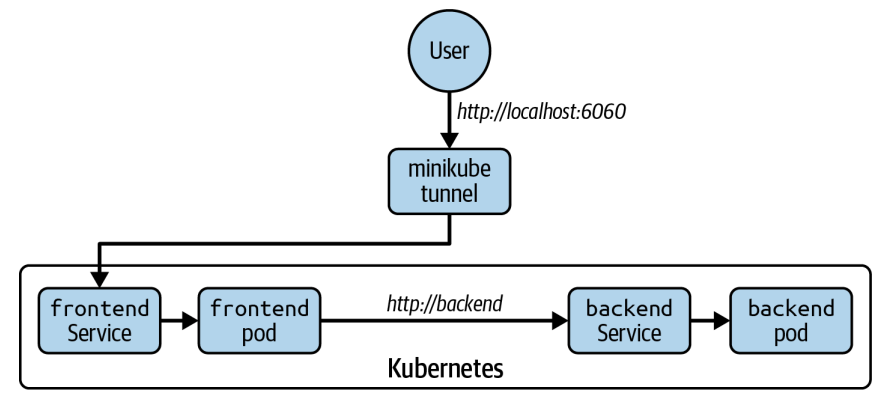
\includegraphics[width=1\linewidth]{Pics/kb1}
		\caption{\label{fig:kb1} Kịch bản một.}
		\label{fig:kb1}
	\end{figure}
	
	\hspace{1.0cm}{Ở trong kịch bản này, mục tiêu của chúng ta là sẽ tiến hành mã hoá và thiết lập các luật cho microservice. Các cách mã hoá sẽ được giải thích ở phần bên dưới.}
	\subsubsection{Thực nghiệm}
	\hspace{1.0cm}{Đầu tiên, chúng ta có tạo một tệp tin cấu hình của ứng dụng và service dành cho frontend, nội dung của tệp tin đó như sau:}
	\begin{lstlisting}[language=Bash]
		apiVersion: apps/v1
		kind: Deployment
		metadata:
			name: frontend
			labels:
				app: frontend
		spec:
			replicas: 1
			selector:
			matchLabels:
				app: frontend
			template:
				metadata:
					labels:
						app: frontend
				annotations:
					consul.hashicorp.com/connect-inject: 'true'
			spec:
				containers:
				  - name: frontend
				  image: ghcr.io/consul-up/birdwatcher-frontend:1.0.0
				  env:
					- name: BIND_ADDR
					  value: "0.0.0.0:6060"
					- name: BACKEND_URL
					  value: "http://backend"
				  ports:
				    - containerPort: 6060
	\end{lstlisting}

	\begin{lstlisting}[language=Bash]
		apiVersion: v1
		kind: Service
		metadata:
			name: frontend
				labels:
					app: frontend
		spec:
			type: LoadBalancer
			selector:
				app: frontend
			ports:
				- protocol: TCP
				  port: 6060
				  targetPort: 6060
	\end{lstlisting}
	\hspace{1.0cm}{Ở bên trên, lần lượt là nội dung của cấu hình dành cho ứng dụng frontend. Ứng dụng sẽ được triển khai theo kiểu deployment, tên của deployment là frontend và được gán label với key là app và value là frontend. Tiếp theo, số lượng pod được sao chép nhau được định nghĩa là 1, và bên số lượng bản sao sẽ có cùng một cấu hình được mô phỏng theo trường template ở bên dưới. Ứng dụng sẽ được thêm một trường annotation, trường này sẽ có tác dụng ghi đè cấu hình của Consul lên trên ứng dụng. Ở đây, chúng ta sẽ truyền vào annotaions là pod sẽ được inject sidecar đi kèm với ứng dụng. Cuối cùng, phần ứng dụng sẽ là một image có tên là \textit{ghcr.io/consul-up/birdwatcher-frontend:1.0.0}, các bản sao sẽ dựa trên image này và bắt đầu khởi chạy ứng dụng. Các biến môi trường được truyền vào theo kiểu khoá và giá trị, các giá trị này sẽ giúp cho ứng dụng chạy trên ip là 0.0.0.0 với cổng là 6060 và đường dẫn tới ứng dụng backend là \textit{http://backend}. Cổng của ứng dụng sẽ được mở là cổng 6060.}
	
	\hspace{0.3cm}{Với tệp cấu hình service, chúng ta sẽ tạo cho ứng dụng một service có tên là frontend, loại của service này là \textit{LoadBalancer}, giao thức của ứng dụng này được sử dụng là TCP, cổng của service là 6060 và cổng của container được service trỏ vào là 6060.}
	
	\hspace{0.3cm}{Tiếp theo đấy, là tệp tin cấu hình của ứng dụng và service dành cho  backend, tệp tin có nội dung như sau:}
		\begin{lstlisting}[language=Bash]
		apiVersion: apps/v1
		kind: Deployment
		metadata:
			name: backend
				labels:
					app: backend
		spec:
			replicas: 1
			selector:
				matchLabels:
					app: backend
			template:
				metadata:
					labels:
						app: backend
				annotations:
					consul.hashicorp.com/connect-inject: 'true'
				spec:
					containers:
					  - name: backend
				 	  image: ghcr.io/consul-up/birdwatcher-frontend:1.0.0
					  env:
						- name: BIND_ADDR
						  value: "0.0.0.0:7000"
					  ports:
					  	- containerPort: 7000
	\end{lstlisting}

	\begin{lstlisting}[language=Bash]
		apiVersion: v1
		kind: Service
		metadata:
			name: backend
				labels:
					app: backend
		spec:
			type: LoadBalancer
				selector:
					app: backend
			ports:
				- protocol: TCP
				  port: 80
				  targetPort: 7000
	\end{lstlisting}
	\hspace{1.0cm}{Tương tự như frontend, ứng dụng backend sẽ được cấu hình theo kiểu Deployment. Tên của deployment là backend và được gán label với key là app và value là backend. Tiếp theo, số lượng pod được sao chép nhau được định nghĩa là 1, và bên số lượng bản sao sẽ có cùng một cấu hình được mô phỏng theo trường template ở bên dưới. Ứng dụng sẽ được thêm một trường annotation, trường này sẽ có tác dụng ghi đè cấu hình của Consul lên trên ứng dụng. Ở đây, chúng ta sẽ truyền vào annotaions là pod sẽ được inject sidecar đi kèm với ứng dụng. Cuối cùng, phần ứng dụng sẽ là một image có tên là \textit{ghcr.io/consul-up/birdwatcher-backend:1.0.0}, các bản sao sẽ dựa trên image này và bắt đầu khởi chạy ứng dụng. Các biến môi trường được truyền vào theo kiểu khoá và giá trị, các giá trị này sẽ giúp cho ứng dụng chạy trên ip là 0.0.0.0 với cổng là 7000. Cổng của ứng dụng sẽ được mở là cổng 7000.}

	\hspace{0.3cm}{Với tệp cấu hình service, chúng ta sẽ tạo cho ứng dụng một service có tên là backend, loại của service này không được định nghĩa, nên kubernetes sẽ tự ngầm hiểu là kiểu \textit{ClusterIP}, giao thức của ứng dụng này được sử dụng là TCP, cổng của service là 80 và cổng của container được service trỏ vào là 7000.}
	
	\hspace{0.3cm}{Sau khi chúng ta có sao chép nội dung vào các tệp tin, chúng ta sẽ di chuyển chúng vào trong một thư mục. Ở đây, chúng ta sẽ di chuyển vào thư mục \textit{/c/Users/justo/Desktop/Helm-chart/nestjs-helm/consul/manifest/application}. Để chạy các ứng dụng, chúng ta sẽ bắt sử dụng câu lệnh sau:}
	\begin{lstlisting}[language=Bash]
	kubectl apply -f /c/Users/justo/Desktop/Helm-chart/nestjs-helm/consul/manifest/application/. 
	\end{lstlisting}

	\hspace{1.0cm}{Sau khi apply, ứng dụng sẽ được triển khai trên sẽ mất một thời gian để ở trạng thái ready. Để kiểm tra trạng thái ứng dụng, chúng ta sẽ chạy lệnh sau:}
	\begin{lstlisting}[language=Bash]
	$ kubectl get deployment,service --selector app=frontend
	NAME                       READY   UP-TO-DATE   AVAILABLE   AGE
	deployment.apps/frontend   1/1     1            1           2d20h
	
	NAME               TYPE           CLUSTER-IP      EXTERNAL-IP   PORT(S)          AGE
	service/frontend   LoadBalancer   10.110.206.79   localhost     6060:32589/TCP   2d20h
	\end{lstlisting}
	\begin{lstlisting}[language=Bash]
	$ k get deployment,service --selector app=backend
	NAME                      READY   UP-TO-DATE   AVAILABLE   AGE
	deployment.apps/backend   1/1     1            1           2d20h
	
	NAME              TYPE        CLUSTER-IP     EXTERNAL-IP   PORT(S)   AGE
	service/backend   ClusterIP   10.103.28.18   <none>        80/TCP    2d20h
	\end{lstlisting}

	\hspace{0.3cm}{Ở đây, con số của trạng thái sẵn sàng là 1/1, thì ứng dụng của chúng ta đã được triển khai thành công. Service của các ứng dụng đã được mở cổng như chúng ta mong đợi. Và tiếp theo, chúng ta sẽ bắt đầu truy cập vào UI của ứng dụng frontend và xem kết quả.}
	
	\hspace{0.3cm}{Để truy cập được vào UI của ứng dụng, chúng ta sẽ sử dụng câu lệnh port-forward để mở port của ứng dụng ra bên ngoài máy của chúng ta. Câu lệnh được thực thi như sau:}
	\begin{lstlisting}[language=Bash]
	kubectl port-forward service/frontend 6060
	\end{lstlisting}
	\hspace{1.0cm}{Sau khi port-forward thành công, chúng ta mở trình duyệt web lên và tiến hành truy cập vào địa chỉ \textit{http://localhost:6060} để kiểm tra kết quả.}
	\pagebreak
	
	\begin{figure}[h]
		\centering
		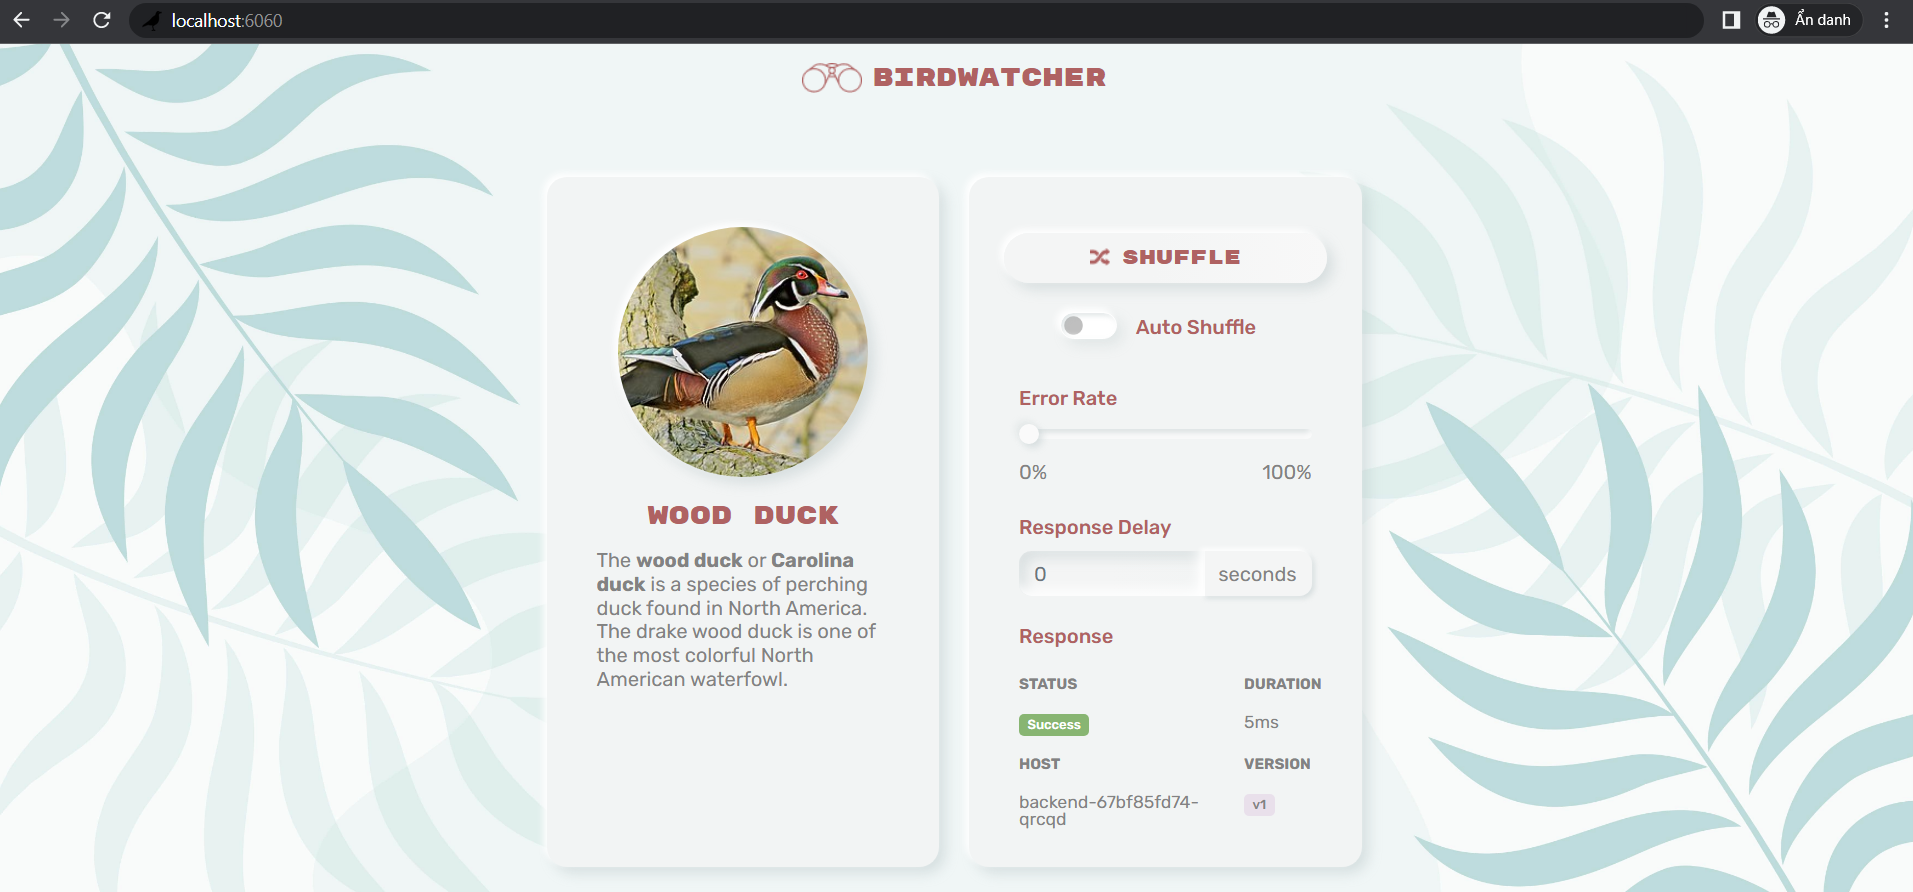
\includegraphics[width=1\linewidth]{Pics/localhost-6060}
		\caption{\label{fig:localhost-6060} Giao diện ứng dụng frontend.}
		\label{fig:localhost-6060}
	\end{figure}

	\hspace{0.3cm}{Tiếp theo, chúng ta đã thêm annotations vào trong tệp cấu hình, chúng ta sẽ port-forward tiếp consul server tương tự như trên và chúng ta tiến hành vào giao diện của consul với địa chỉ \textit{http://localhost:8500} để xem kết quả mà chúng ta đã truyền sidecar đi kèm với ứng dụng.}
	
	\begin{figure}[h]
		\centering
		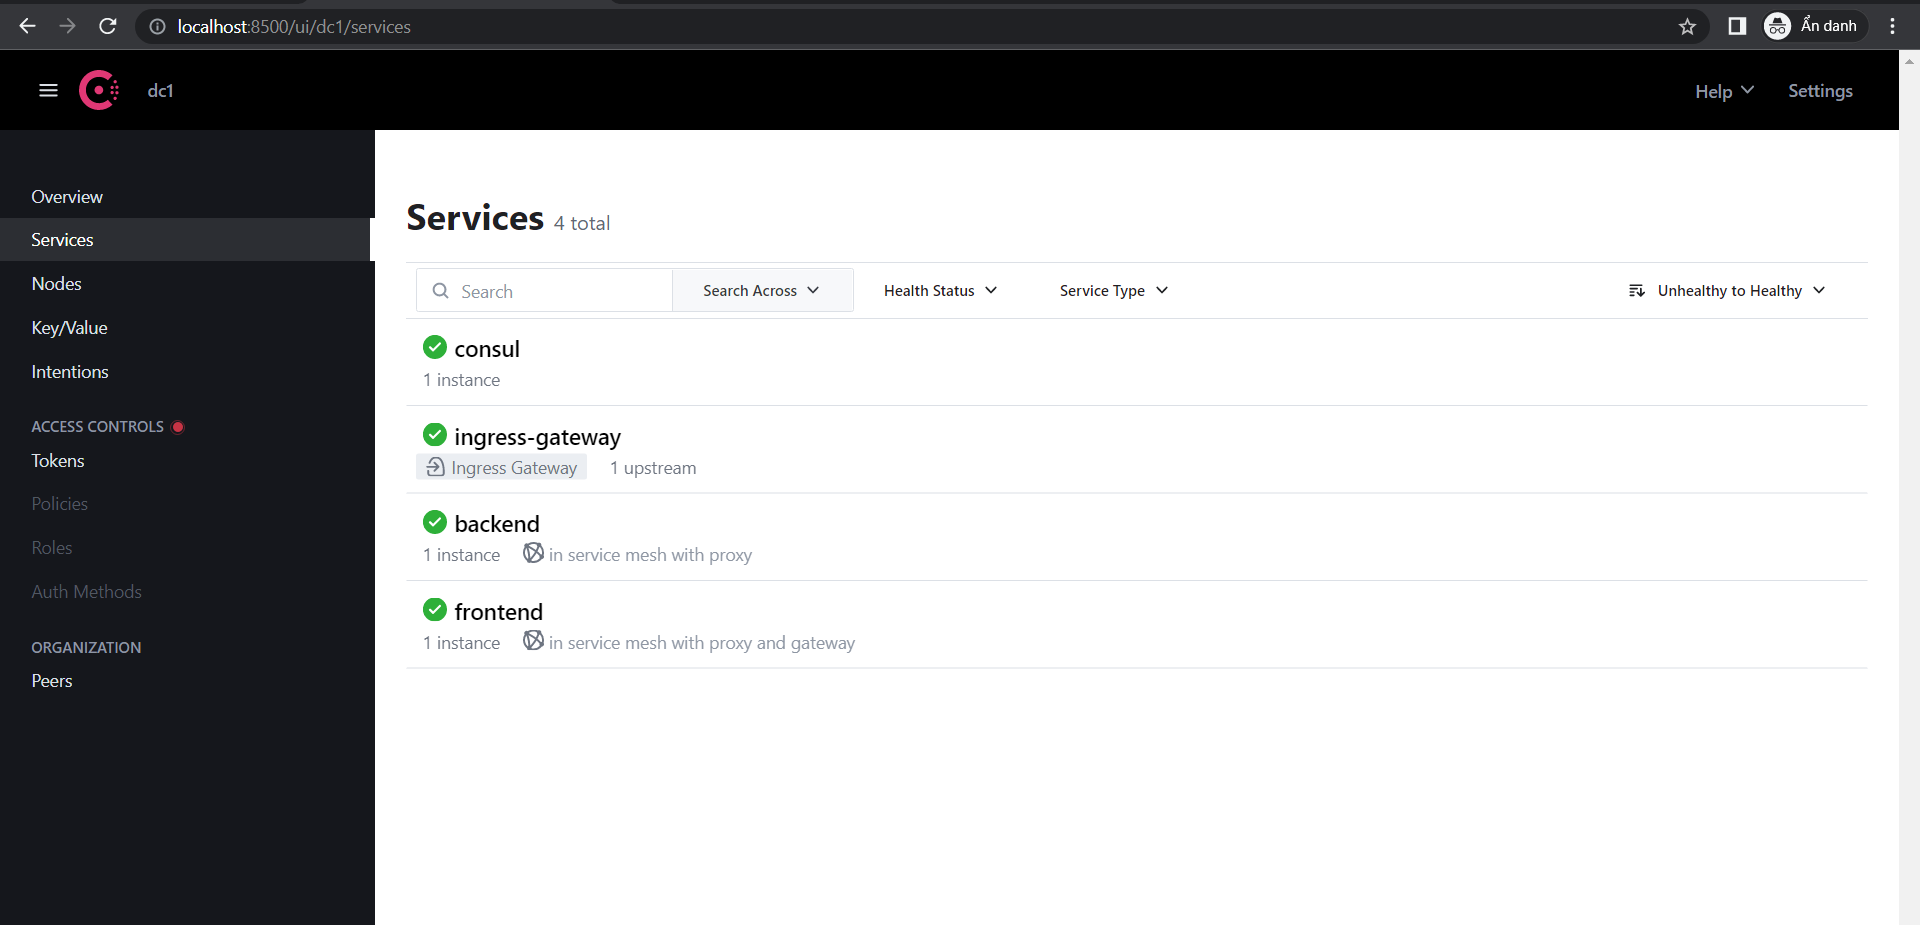
\includegraphics[width=1\linewidth]{Pics/localhost-8500}
		\caption{\label{fig:localhost-8500} Giao diện Consul Server.}
		\label{fig:localhost-8500}
	\end{figure}
	\hspace{0.3cm}{Như vậy, chúng ta đã thành công truyền proxy đi kèm với ứng dụng frontend và backend, hay nói cách khác, ứng dụng frontend và backend đang là một phần của service mesh. Sau đấy, chúng ta sẽ quay lại trang web \textit{http://localhost:6060} lúc nãy, tải lại trang và kiểm tra kết quả. Nếu như trang trả lại lỗi như bên dưới, thì mọi thứ vẫn đang đúng như những gì chúng ta đã làm.}
	\pagebreak
	\begin{figure}[h]
		\centering
		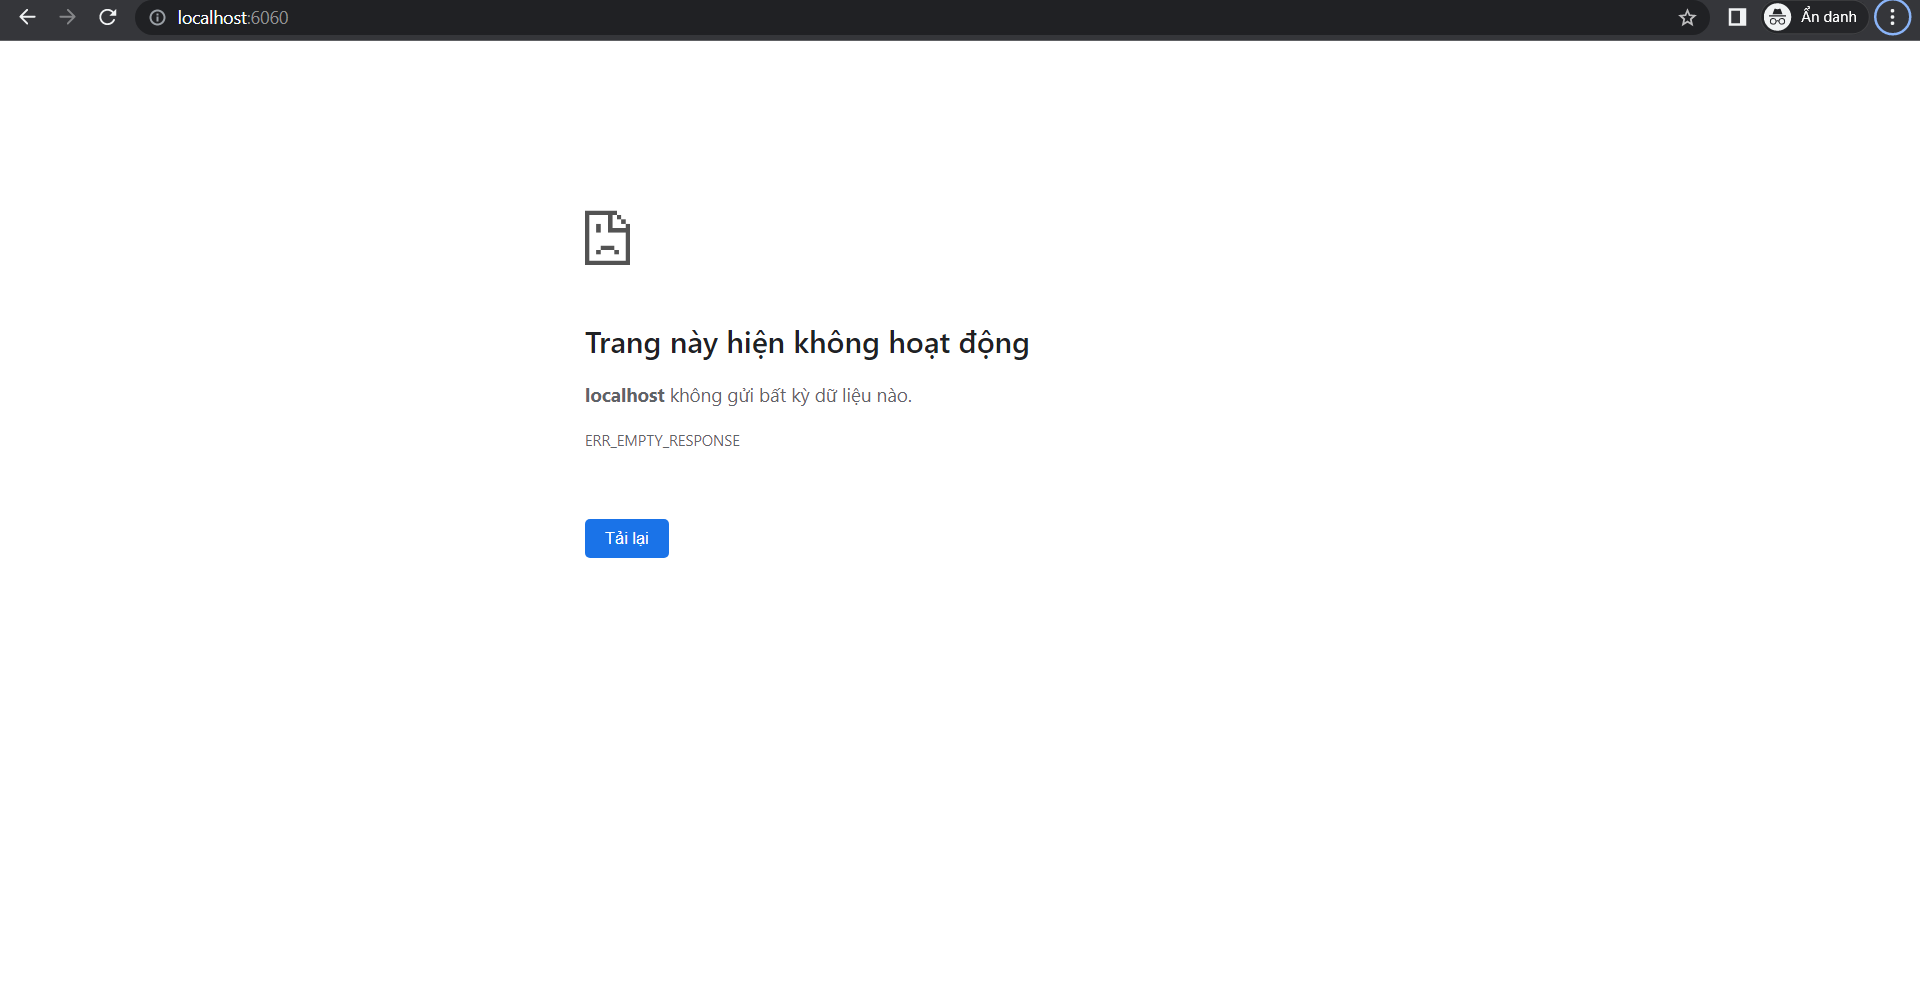
\includegraphics[width=1\linewidth]{Pics/localhost-6060-error}
		\caption{\label{fig:localhost-6060-error} Lỗi khi vào tải lại trang.}
		\label{fig:localhost-6060-error}
	\end{figure}

	\hspace{0.3cm}{Lý do mà trang không thể tải lại được, nguyên nhân là do ứng dụng frontend đang là một phần của service mesh. Sidecar proxy đã chặn tất cả các nguồn đi vào được trong ứng dụng. Consul đã bảo mật ứng dụng và yêu cầu tất cả các luồng đi vào service mesh cần phải được xác thực và uỷ quyền.  Khi mà chúng ta request tới frontend, thì chúng ta chưa xác thực và nhận được quyền truy cập vào trong frontend nên Consul đã từ chối và không cho phép chúng ta truy cập. Nếu như chúng ta truy cập được bằng port-forward, thì portforward đã cho phép chúng ta bỏ qua luật của consul và truy cập thẳng vào trong ứng dụng frontend.}
	
	\hspace{0.3cm}{Ở trên giao diện của Consul, chúng ta click vào các service, ở đây, giao diện sẽ hiện ra các cấu trúc giữa các service mesh với nhau.}
	
	\begin{figure}[h]
		\centering
		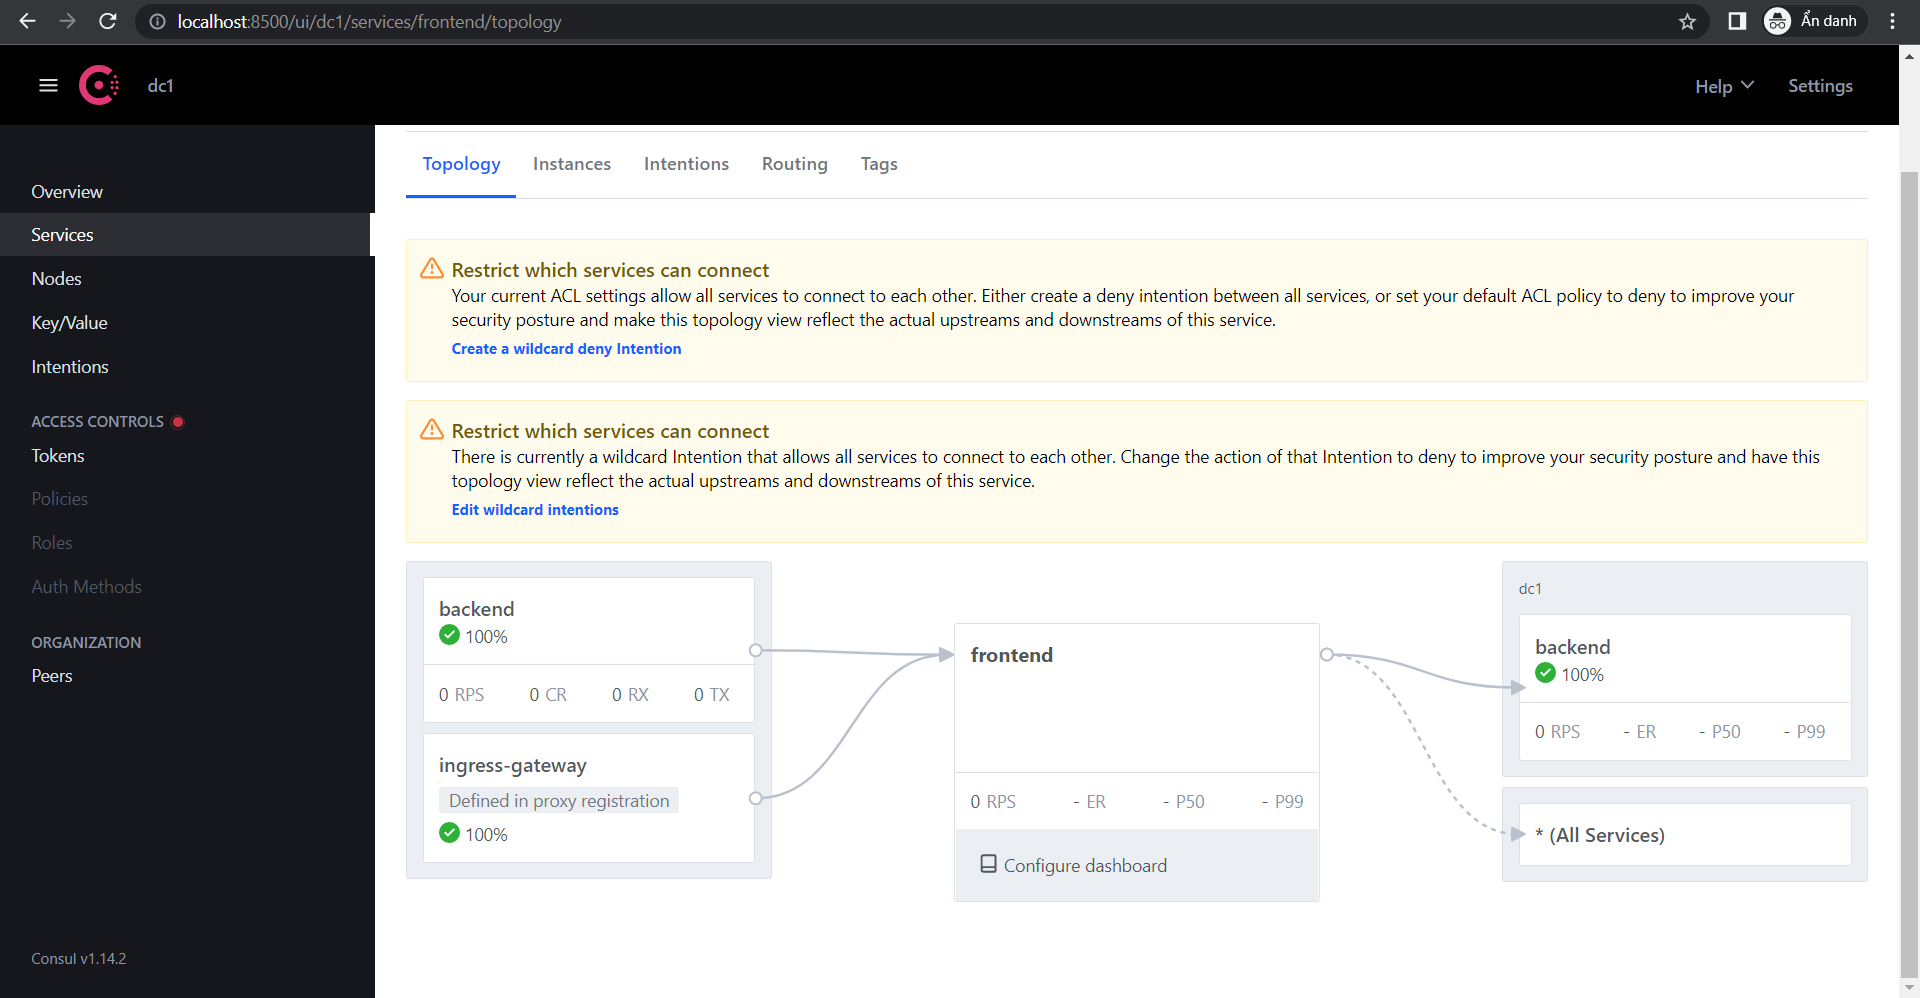
\includegraphics[width=1\linewidth]{Pics/topology}
		\caption{\label{fig:topology} Cấu trúc của service frontend.}
		\label{fig:topology}
	\end{figure}
	
	\hspace{0.3cm}{Tiếp theo, chúng ta sẽ tiến hành thiết lập luật dành cho service frontend và backend. Để thiết lập, chúng ta có 2 cách để làm, cách thứ nhất là chúng ta có thể làm trực tiếp trên giao diện, nhưng mà chúng ta không nên sử dụng cách này, vì sau khi chúng ta di dời Consul sang một bên khác, thì chúng ta sẽ lại phải thiết lập bằng tay tất cả các service. Việc này khá là tốn effort dành cho người quản trị. Với cách thứ hai, chúng ta có thể viết cấu hình vào một tiệp loại yaml dành cho kubernetes. Tệp cấu hình có nội dung như sau:}
	\begin{lstlisting}[language=Bash]
		apiVersion: consul.hashicorp.com/v1alpha1
		kind: ServiceIntentions
		metadata:
			name: frontend
			namespace: consul
		spec:
			destination:
			  name: frontend
			sources:
			- name: backend
			  action: allow
	\end{lstlisting}
	\hspace{1.0cm}{Sau khi tạo một tệp với nội dung bên trên, chúng ta tiến hành apply nó và lên trên giao diện của Consul Server và xem kết quả.}
	
	\begin{figure}[h]
		\centering
		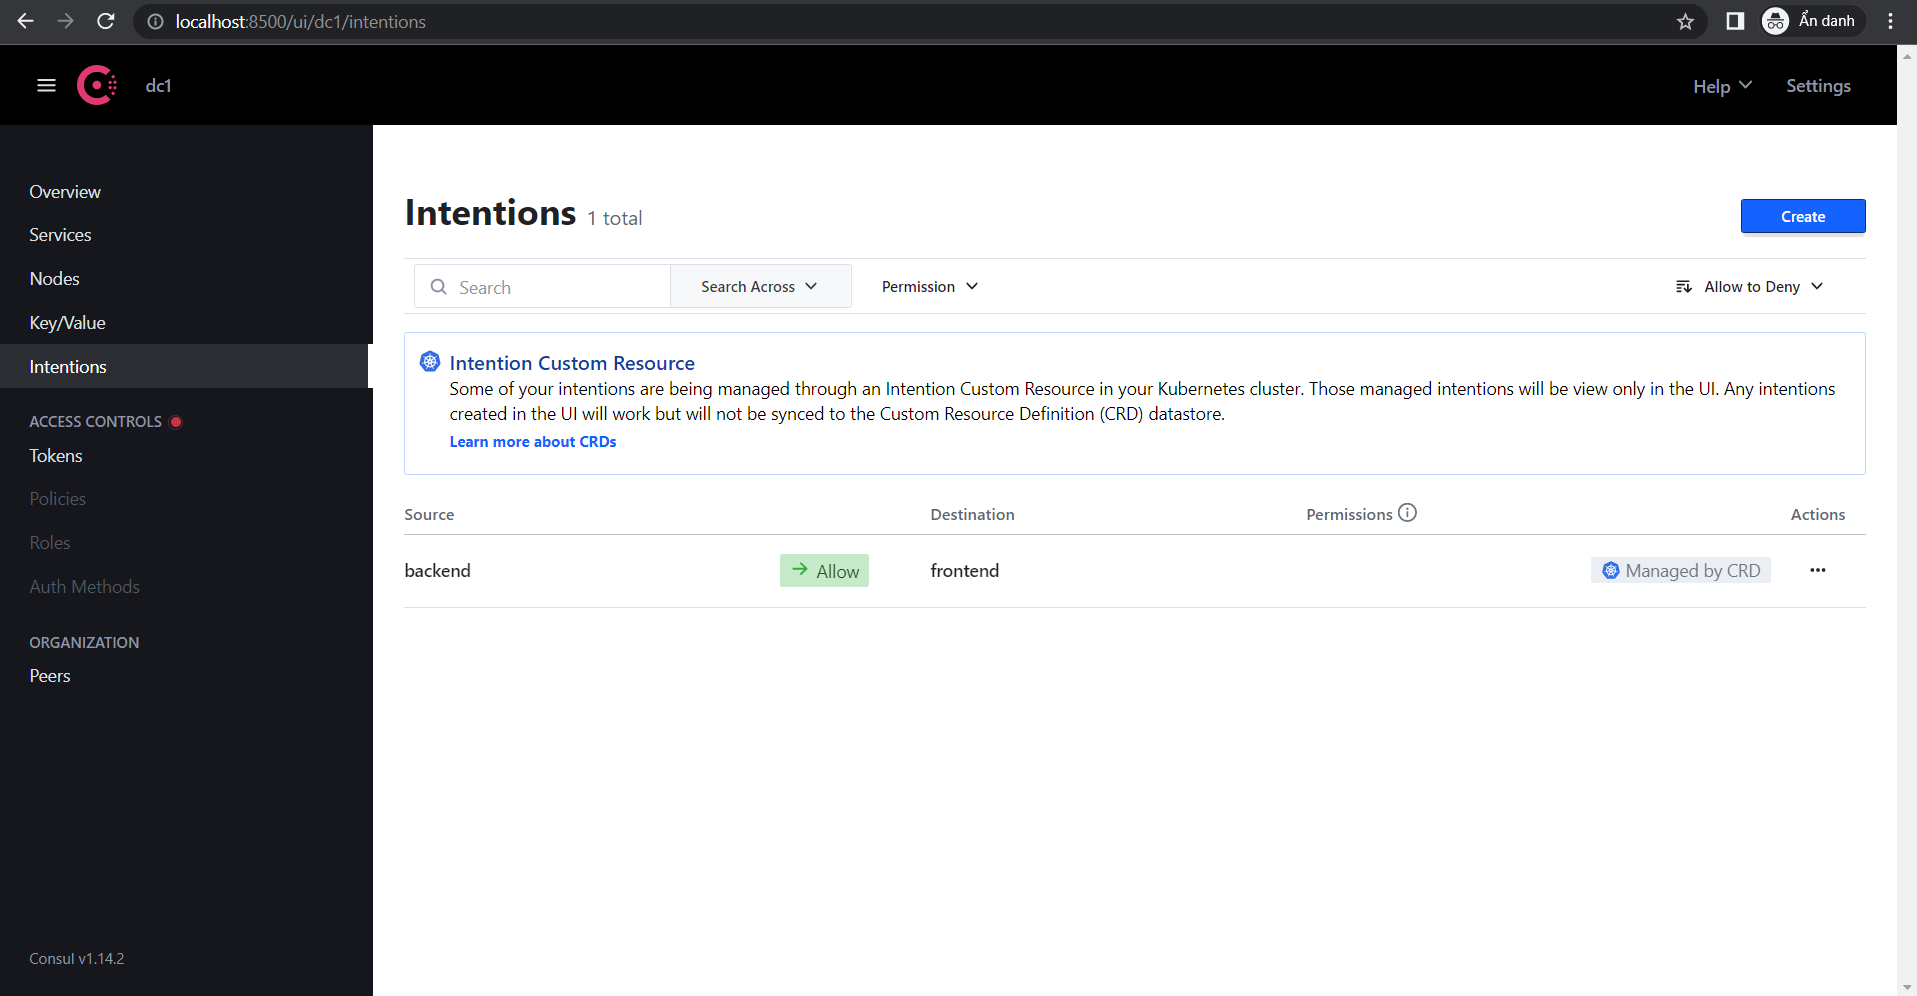
\includegraphics[width=1\linewidth]{Pics/intention-1}
		\caption{\label{fig:intention-1} Intention sau khi được cấu hình.}
		\label{fig:intention-1}
	\end{figure}

	\hspace{0.3cm}{Với luật này, chúng ta cho phép service backend được kết nối tới service frontend. Tuy nhiên, đến đây vẫn chưa xong, vì mặc định của proxy là giao tiếp thông qua giao thức tcp, mà ứng dụng frontend và backend giao tiếp thông qua giao thức http. Vì vậy, chúng ta cần cài đặt lại để cho proxy nhận truy cập http. Để cấu hình, chúng ta cần tạo 1 tệp tin với nội dung như sau:}
	\begin{lstlisting}[language=Bash]
	apiVersion: consul.hashicorp.com/v1alpha1
	kind: ProxyDefaults
	metadata:
		name: global
		namespace: consul
	spec:
		config:
		protocol: http
	\end{lstlisting}
	\hspace{1.0cm}{Sau khi cấu hình xong, chạy lệnh sau để kiểm tra:}
	\begin{lstlisting}[language=Bash]
	$ kubectl get proxydefaults.consul.hashicorp.com  -A
	NAMESPACE   NAME     SYNCED   LAST SYNCED   AGE
	consul      global   True     90m           90m
	\end{lstlisting}
	\hspace{1.0cm}{Như vậy, với status là synced, thì có nghĩa là ứng dụng đã có thể giao tiếp với nhau thông qua giao thức http.}
	
	\hspace{0.3cm}{Tiếp theo đấy, chúng ta sẽ kiểm tra xem thông tin chứng chỉ mà Consul tạo ra cho ứng dụng. Để kiểm tra, đầu tiên chúng ta cần truy cập được vào trong container ứng dụng với câu lệnh sau:}
	\begin{lstlisting}[language=Bash]
		kubectl exec deploy/backend -c backend -- \
		sh -c 'openssl s_client -connect $(hostname -i):20000 | \
		openssl x509 -noout -text'
		--------------------------------------------
		openssl x509 -noout -text'
		Can't use SSL_get_servername
		depth=0
		verify error:num=20:unable to get local issuer certificate
		verify return:1
		depth=0
		verify error:num=21:unable to verify the first certificate
		verify return:1
		depth=0
		verify return:1
		DONE
		Certificate:
		Data:
		Version: 3 (0x2)
		Serial Number: 39 (0x27)
		Signature Algorithm: ecdsa-with-SHA256
		Issuer: CN = pri-1r5tjaui.consul.ca.562ec48b.consul
		Validity
		Not Before: Dec 20 13:12:29 2022 GMT
		Not After : Dec 23 13:12:29 2022 GMT
		Subject:
		Subject Public Key Info:
		Public Key Algorithm: id-ecPublicKey
		Public-Key: (256 bit)
		pub:
		04:1c:cd:db:7b:49:00:e2:9a:48:97:71:31:88:32:
		45:85:c8:15:01:82:b9:27:34:eb:0b:a0:63:02:7d:
		fe:1e:af:a2:42:e8:26:1f:19:43:2a:51:d5:bf:46:
		42:0f:f5:65:36:29:2d:05:ff:80:d4:23:93:49:00:
		18:1f:44:1f:dd
		ASN1 OID: prime256v1
		NIST CURVE: P-256
		X509v3 extensions:
		X509v3 Key Usage: critical
		Digital Signature, Key Encipherment, Data Encipherment, Key Agreement
		X509v3 Extended Key Usage:
		TLS Web Client Authentication, TLS Web Server Authentication
		X509v3 Basic Constraints: critical
		CA:FALSE
		X509v3 Subject Key Identifier:
		BB:38:30:7C:86:88:A3:DC:AB:43:69:77:6B:B9:43:95:81:D1:25:47:E4:FA:9C:D6:AB:C2:A1:FE:99:51:FA:F7
		X509v3 Authority Key Identifier:
		keyid:0B:A1:BC:23:3F:15:0E:84:6B:32:30:E2:03:42:68:1B:2B:99:FF:7F:78:F1:71:0B:9D:70:5A:C0:F0:DE:66:A0
		
		X509v3 Subject Alternative Name: critical
		URI:spiffe://562ec48b-2872-87db-c307-d5435d3d833e.consul/ns/default/dc/dc1/svc/backend
		Signature Algorithm: ecdsa-with-SHA256
		30:45:02:21:00:ed:64:a1:78:0e:09:8b:fc:6c:ea:10:76:5b:
		57:c5:a3:c5:8c:0d:b2:ab:65:12:a1:67:45:0f:31:7d:dc:fd:
		74:02:20:15:ab:1c:60:c6:64:91:2e:0f:0b:bb:47:33:a2:24:
		13:54:3d:0a:fe:3b:8f:c6:e7:53:ea:e2:47:c6:65:75:79
	\end{lstlisting}
	\hspace{1.0cm}{Đây là chứng chỉ mà Consul tạo ra để mã hoá các dữ liệu được truyền qua nhau thông qua proxy. Các chứng chỉ này được tạo ra bởi Consul, ở đây Consul đóng vai trò là một cơ quan cấp chứng chỉ và cấp cho mỗi Service. Dưới đây là cách mà Consul tạo ra chứng chỉ để mã hoá và dùng chứng chỉ để giải mã dữ liệu.}
	\pagebreak
	\begin{figure}[h]
		\centering
		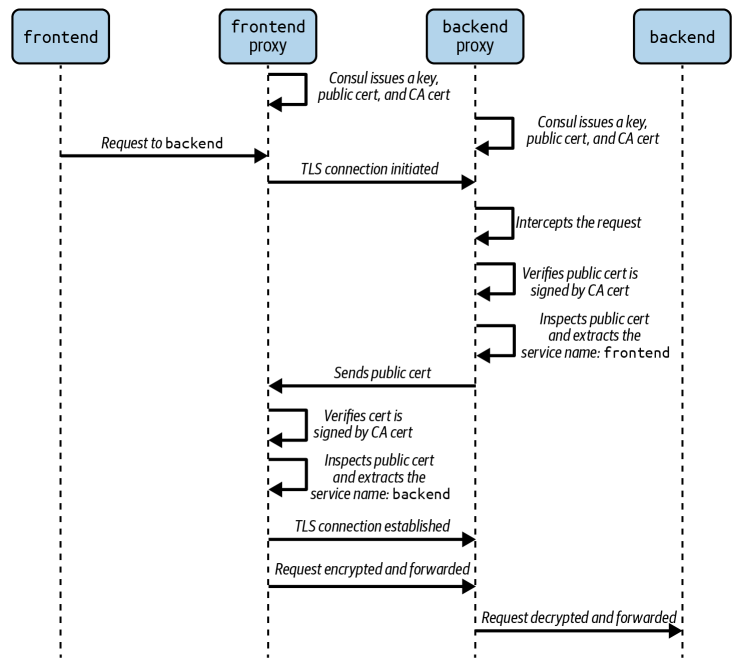
\includegraphics[width=1\linewidth]{Pics/certificate}
		\caption{\label{fig:certificate} Biểu đồ tuần tự trong giao tiếp của ứng dụng frontend và backend.}
		\label{fig:certificate}
	\end{figure}

	\hspace{0.3cm}{Với mỗi chứng chỉ, Consul sẽ mã hoá ID của mỗi service được gọi là SPIFFE ID, mỗi ID được gắn vào chứng chỉ và chỉ có Consul có thể giải mã được được ID đấy. Cho nên, nếu như hacker có thể xâm nhập được vào ứng dụng, nhưng khi gọi các service, hacker sẽ không có được ID để mã hoá và gửi cho các service kia.}
	\subsubsection{Đánh giá}
	\hspace{1.0cm}{Qua kịch bản trên, chúng ta đã có thể mã hoá giao tiếp giữa các service với nhau thông qua TLS cũng như thiết lập các luật giao tiếp của chúng với nhau. Tuy nhiên, khi mà chúng ta thiết lập xong như vậy, thì làm thế nào để chúng ta không cần xác thực và được uỷ quyền đến từ consul mà vẫn có thể truy cập được ứng dụng, chúng ta sẽ đến kịch bản 2, triển khai Ingress Gateway cho các service.}
	\subsection{Kịch bản hai: Triển khai ingress gateway cho các service}
	\subsubsection{Mô tả kịch bản}
	\pagebreak
	\begin{figure}[h]
		\centering
		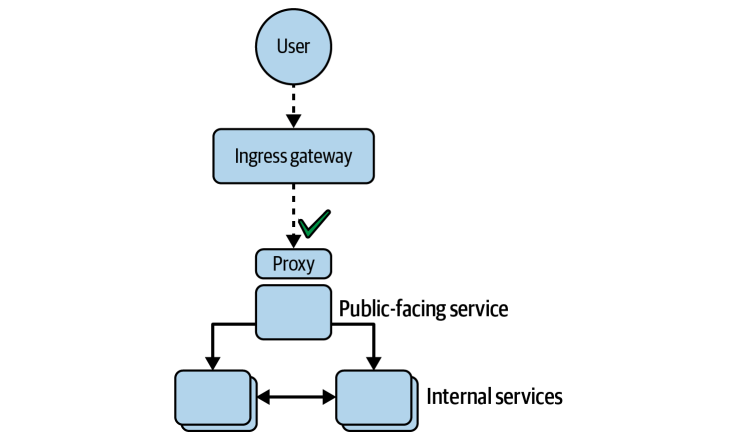
\includegraphics[width=1\linewidth]{Pics/ingress-gateway}
		\caption{\label{fig:ingress-gateway} Luồng truy cập của người dùng vào trong ứng dụng thông qua ingress-gateway.}
		\label{fig:ingress-gateway}
	\end{figure}
	
	\hspace{1.0cm}{Để giúp cho người dùng có thể truy cập được ứng dụng mà không cần sự đồng ý của Consul, thì chúng ta sẽ tiến hành tạo ra một trong những thành phần của Consul là ingress gateway. Ingress gateway ở đây sẽ đóng một vai trò là sẽ điều hướng toàn bộ yêu cầu vào và chuyển các yêu cầu đấy tới các service tương ứng. Vậy làm thế nào để tạo ra ingress gateway, làm sao để có thể điều hướng vào các dịch vụ tương ứng, chúng ta sẽ đến với phần thực nghiệm.}
	
	\subsubsection{Thực nghiệm}
	\hspace{1.0cm}{Đầu tiên, để tạo ra ingress gateway, thì chúng ta cần cập nhật tệp tin values.yaml ở phần các bước triển khai. Chúng ta sẽ thêm vào một phần sau vào bên dưới tệp:}
	\begin{lstlisting}[language=Bash]
	ingressGateways:
		enabled: true
		defaults:
			replicas: 1	
			service:
				type: LoadBalancer
	\end{lstlisting}
	\hspace{1.0cm}{Sau khi thêm vào, chúng ta sẽ chạy câu lệnh sau để update chart của Consul}
	\begin{lstlisting}[language=Bash]
	helm upgrade -n consul consul -f /c/Users/justo/Desktop/Helm-chart/nestjs-helm/consul/helm/values.yaml hashicorp/consul
	\end{lstlisting}
	\hspace{1.0cm}{Sau khi helm upgrade xong chart, thì chúng ta sẽ truy cập vào giao diện của Consul và xem kết quả:}
	\pagebreak
	\begin{figure}[h]
	\centering
	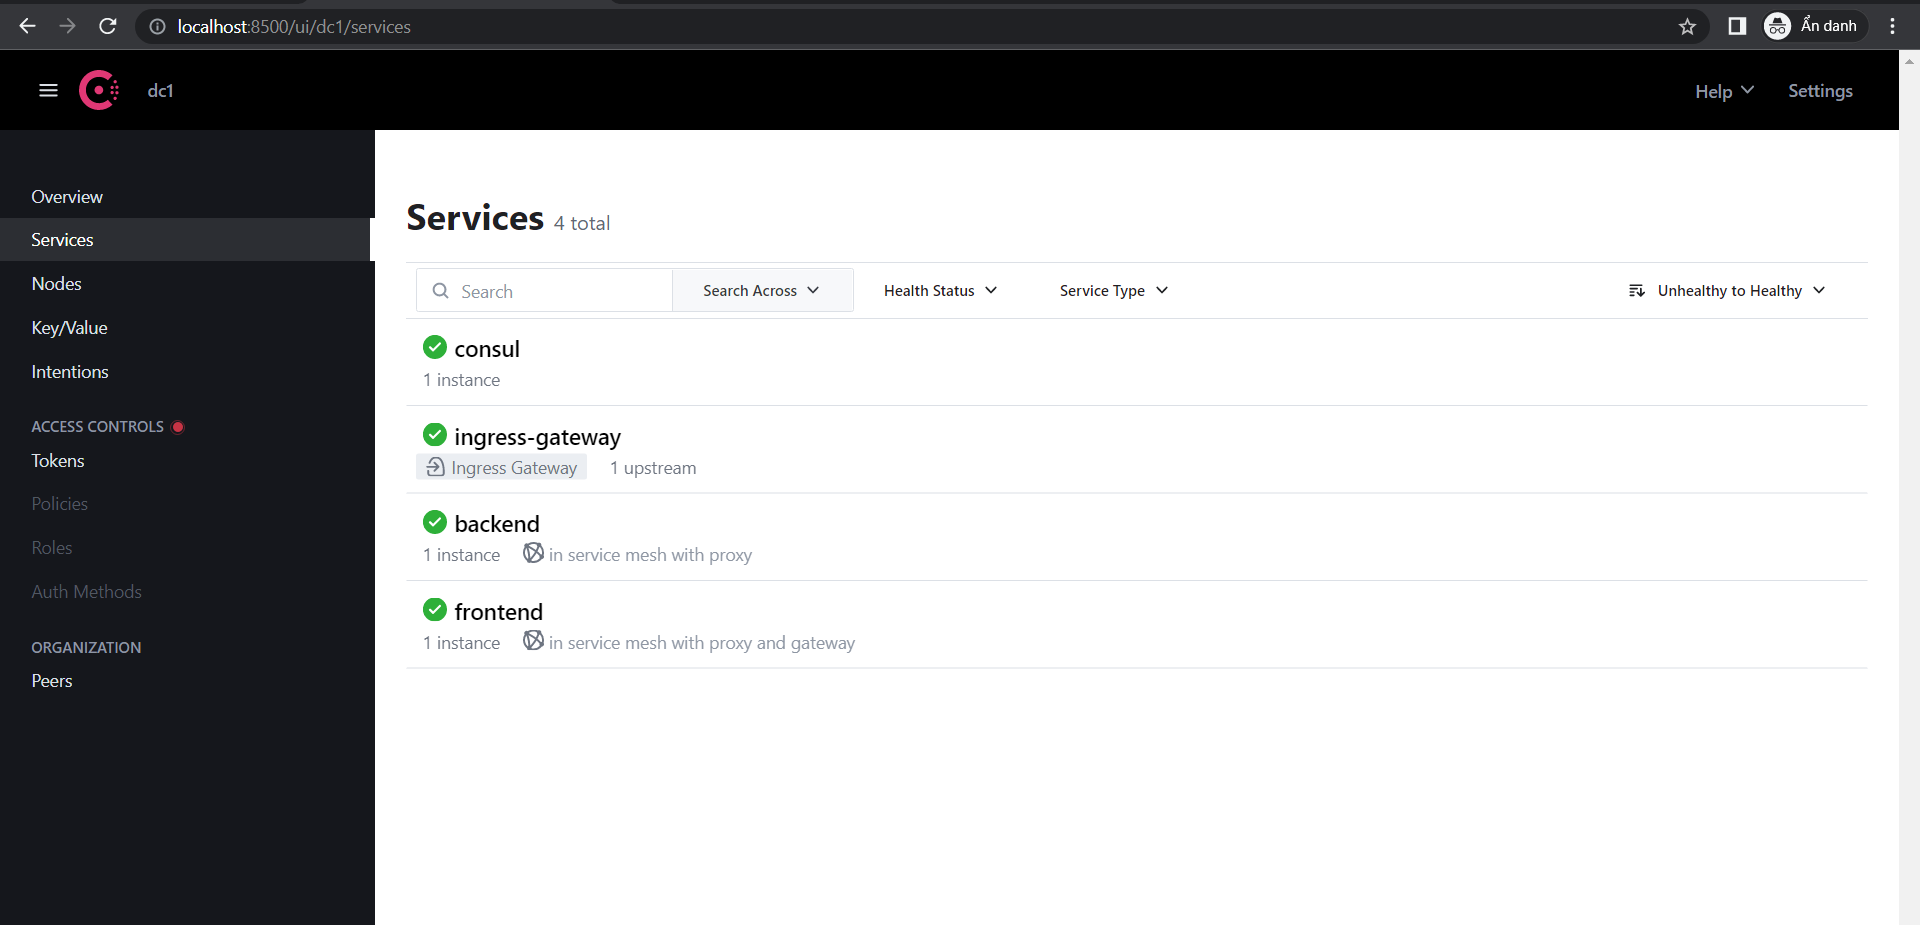
\includegraphics[width=1\linewidth]{Pics/localhost-8500}
	\caption{\label{fig:localhost-8500} Ingress Gateway đã hiện bên trên giao diện.}
	\label{fig:localhost-8500}
	\end{figure}

	\hspace{0.3cm}{Tiếp theo, chúng ta tiến tới cấu hình điều hướng cho người dùng có thể truy cập vào ứng dụng thông qua ingress gateway. Để làm được, chúng ta sẽ có một tệp tin cấu hình của ingress gateway, nội dung của tệp tin như sau:}
	\begin{lstlisting}[language=Bash]
		apiVersion: consul.hashicorp.com/v1alpha1
		kind: IngressGateway
		metadata:
			name: ingress-gateway
			namespace: consul
		spec:
			listeners:
				- port: 8080
				  protocol: http
				  services:
					- name: frontend
					  hosts: ["localhost"]
	\end{lstlisting}
	\hspace{1.0cm}{Khi chúng ta có tệp tin, bắt đầu chạy lệnh để apply nội dung và lên trên UI của Consul để kiểm tra. Để vào xem thông tin, chúng ta vào Service -> Ingress-Gateway -> Upstream và kiểm tra:}
	 \begin{figure}[h]
		\centering
		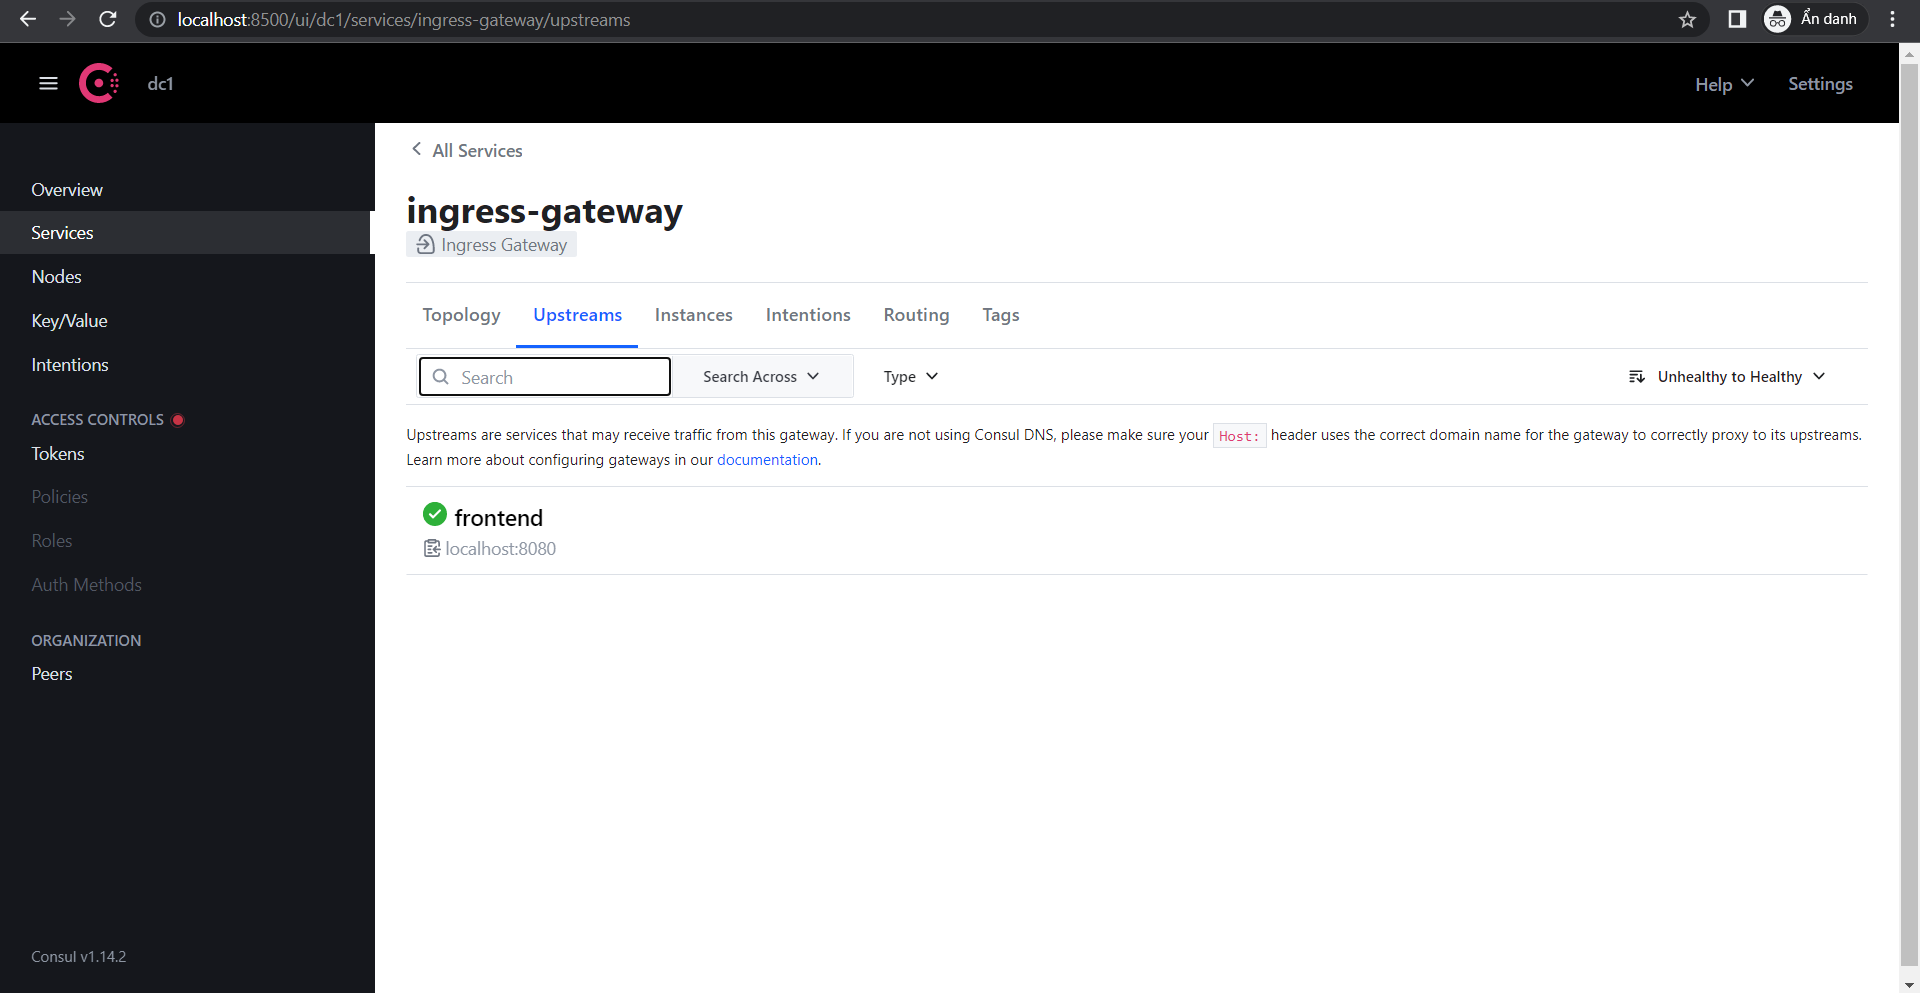
\includegraphics[width=1\linewidth]{Pics/upstream}
		\caption{\label{fig:upstream} Cấu hình điều hướng truy cập tới ứng dụng frontend.}
		\label{fig:upstream}
	\end{figure}
	\hspace{0.3cm}{Như vậy, ứng dụng đã có thể truy cập thông qua ingress gateway. Để truy cập, chúng ta truy cập vào địa chỉ \textit{http://localhost:8080} để kiểm tra.}
	 \begin{figure}[h]
		\centering
		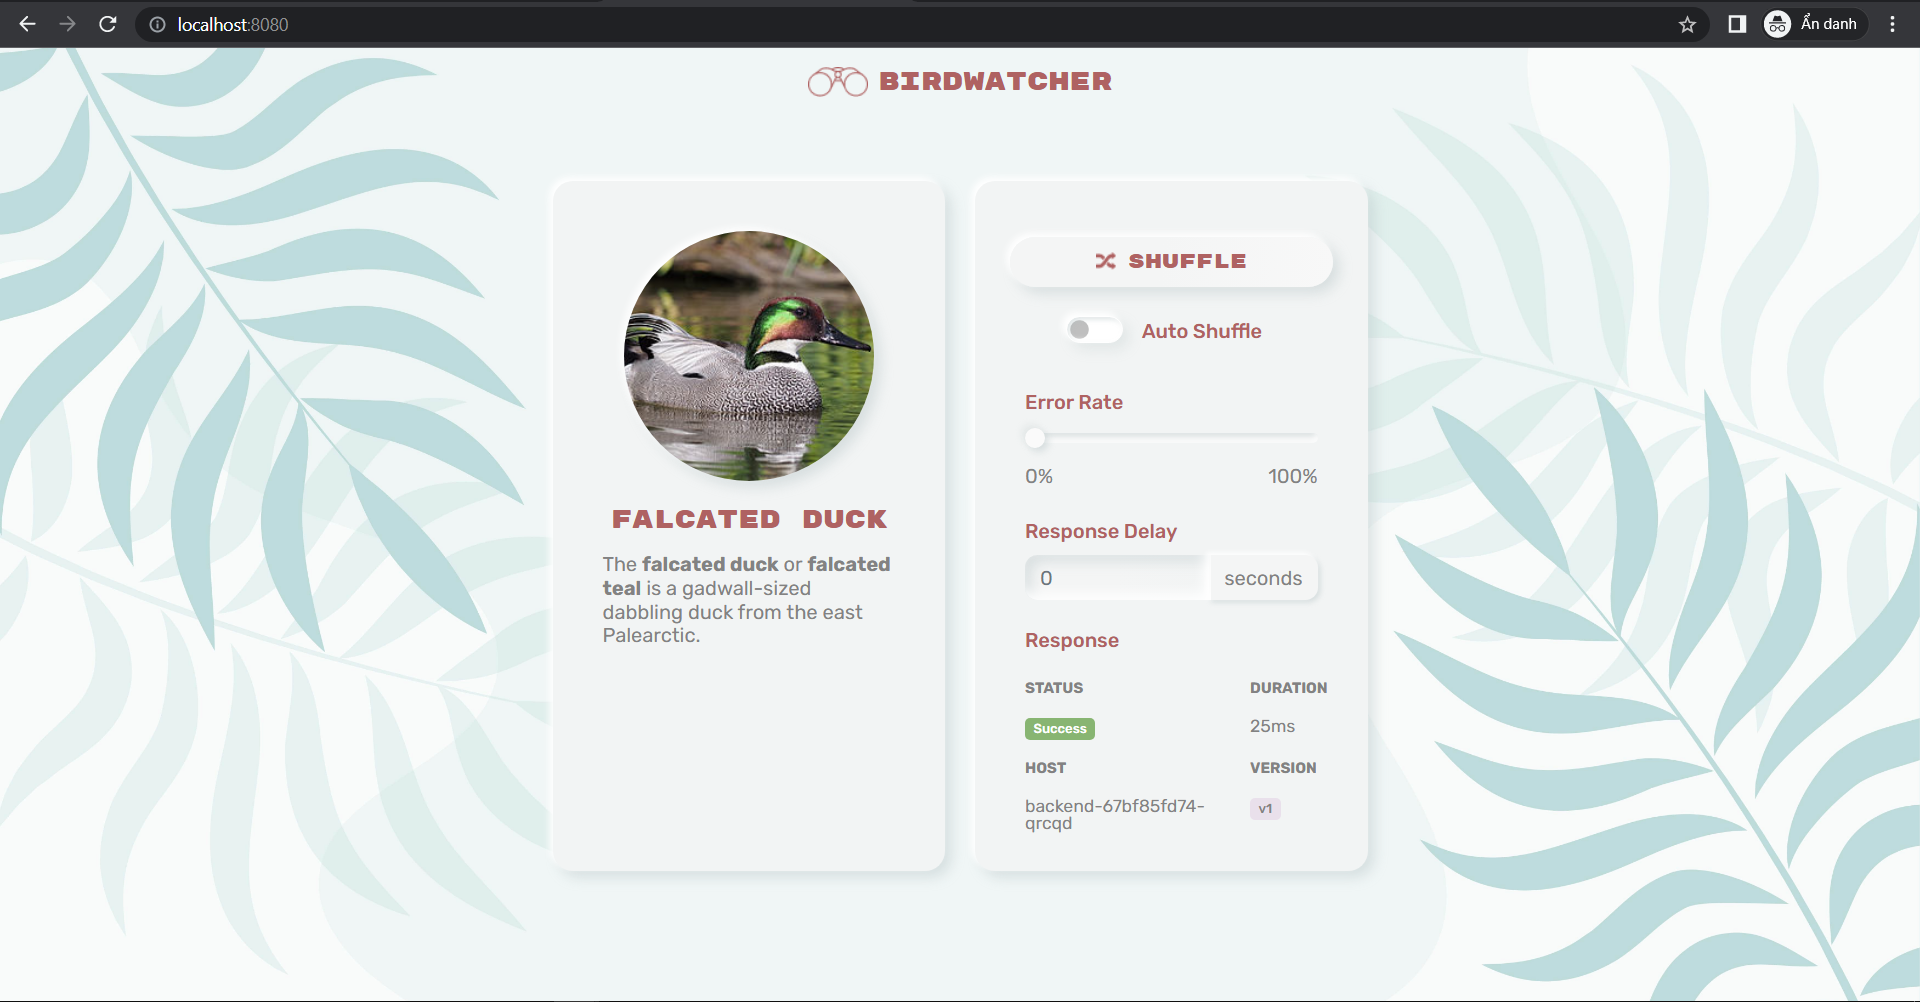
\includegraphics[width=1\linewidth]{Pics/localhost-8080}
		\caption{\label{fig:localhost-8080} Dịch vụ frontend khi được mở thông qua ingress gateway.}
		\label{fig:localhost-8080}
	\end{figure}
	\hspace{0.3cm}{Như vậy chúng ta đã cấu hình thành công để công khai dịch vụ ra ngoài thông qua ingress gateway.}
	\subsubsection{Đánh giá}
	\hspace{1.0cm}{Thông qua triển khai trên, chúng ta đã tiến hành tạo ra ingess gateway để công khai dịch vụ ra ngoài mà không cần phải được quyền cho phép của Consul. Tiếp theo, chúng ta sẽ đến phần điều tra. Khi mà ứng dụng của chúng ta có vấn đề, thì chúng ta cần phải điều tra những nguyên nhân gây ra vấn đề đó. Đó có thể là do Ingress gateway không hoạt động, hay các luật cấu hình sai. Để biết được, chúng ta đến phần tiếp theo, điều tra nguyên nhân gián đoạn của dịch vụ}
	\subsection{Kịch bản ba: Điều tra nguyên nhân gián đoạn dịch vụ}
	\subsubsection{Mô tả kịch bản}
	\begin{figure}[h]
	\centering
	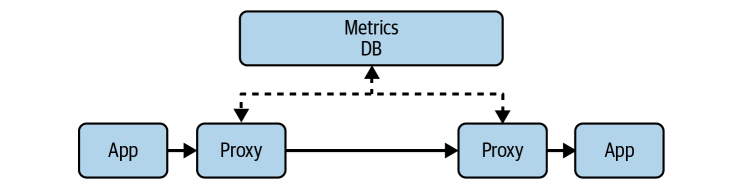
\includegraphics[width=1\linewidth]{Pics/metrics}
	\caption{\label{fig:metrics} Đẩy metrics của proxy lên một Metrics DB.}
	\label{fig:metrics}
	\end{figure}
	\hspace{1.0cm}{Ở phần này, chúng ta sẽ tiến hành đẩy các metrics của proxy lên một nơi có thể đọc được các thông số Metrics. Ở đây, chúng ta sẽ sử dụng Prometheus. Prometheus là một phần đi kèm luôn với chart của Consul. Nếu như chúng ta đã sử dụng Prometheus đã có sẵn, thì chúng ta sẽ không cần phải thêm vào chart và sẽ cấu hình Promtheus có sẵn để thu thập các metrics được đẩy ra bởi proxy. Ở phần thực nghiệm này, chúng ta sẽ sử dụng Prometheus của chart Consul để tiến hành thu thập dữ liệu.}
	\subsubsection{Thực nghiệm}
	\hspace{1.0cm}{Trước khi bắt đầu, chúng ta cần phải triển khai prometheus để thu thập dữ liệu. Để có prometheus, chúng ta sẽ cập nhật lại chart như sau:}
	\begin{lstlisting}[language=Bash]
	prometheus:
		enabled: true
	\end{lstlisting}
	\hspace{1.0cm}{Tiếp đó, chúng ta bắt đầu cấu hình proxy để proxy có thể đẩy các metrics ra bên ngoài. Để cấu hình, tệp values.yaml chúng ta cần chỉnh sửa lại như sau:}
	\begin{lstlisting}[language=Bash]
	connectInject:
		enabled: true
		default: false
		metrics:
			defaultEnabled: true
			defaultEnableMerging: true
			defaultPrometheusScrapePort: 20200
			defaultPrometheusScrapePath: "/metrics"
			defaultMergedMetricsPort: 20100
	\end{lstlisting}
	\hspace{1.0cm}{Với cấu hình trên, chúng ta đã cấu hình đẩy các metrics ra bên ngoài với cổng 20220 và với path là /metrics. Prometheus của Consul sử dụng đã có cấu hình sẵn để thu thập dữ liệu từ cổng và đường dẫn kia nên chúng ta sẽ không cần phải cấu hình lại Prometheus. }
	\hspace{0.3cm}{Tiếp theo, chúng ta sẽ cấu hình để hiển thị thông tin metrics trên UI của Consul. Để làm vậy, chúng ta tiếp tục cập nhật nội dung của tệp values.yaml thành như sau:}
	\begin{lstlisting}[language=Bash]
	ui:
		enabled: true
		service:
			type: NodePort
		metrics:
			provider: "prometheus"
			baseURL: http://prometheus-server
	\end{lstlisting}
	\hspace{1.0cm}{Cấu hình trên, do Promtheus được triển khai ở cùng với namespace Consul, nên chúng ta chỉ cần khai báo tên service của Promtheus là được. Sau đó, chúng ta tiến hành nâng cấp chart để chart nhận config mới với câu lệnh sau:}
	\begin{lstlisting}[language=Bash]
		helm upgrade -n consul consul -f /c/Users/justo/Desktop/Helm-chart/nestjs-helm/consul/helm/values.yaml hashicorp/consul
	\end{lstlisting}
	\hspace{1.0cm}{Vậy là chúng ta đã xong phần triển khai Prometheus cũng như tiến hành đẩy các metrics từ proxy lên Prometheus. Để kiểm tra, chúng ta sẽ port-forward service của Prometheus để kiểm tra trên đường dẫn \textit{http://localhost:9090}.}
	\begin{figure}[h]
		\centering
		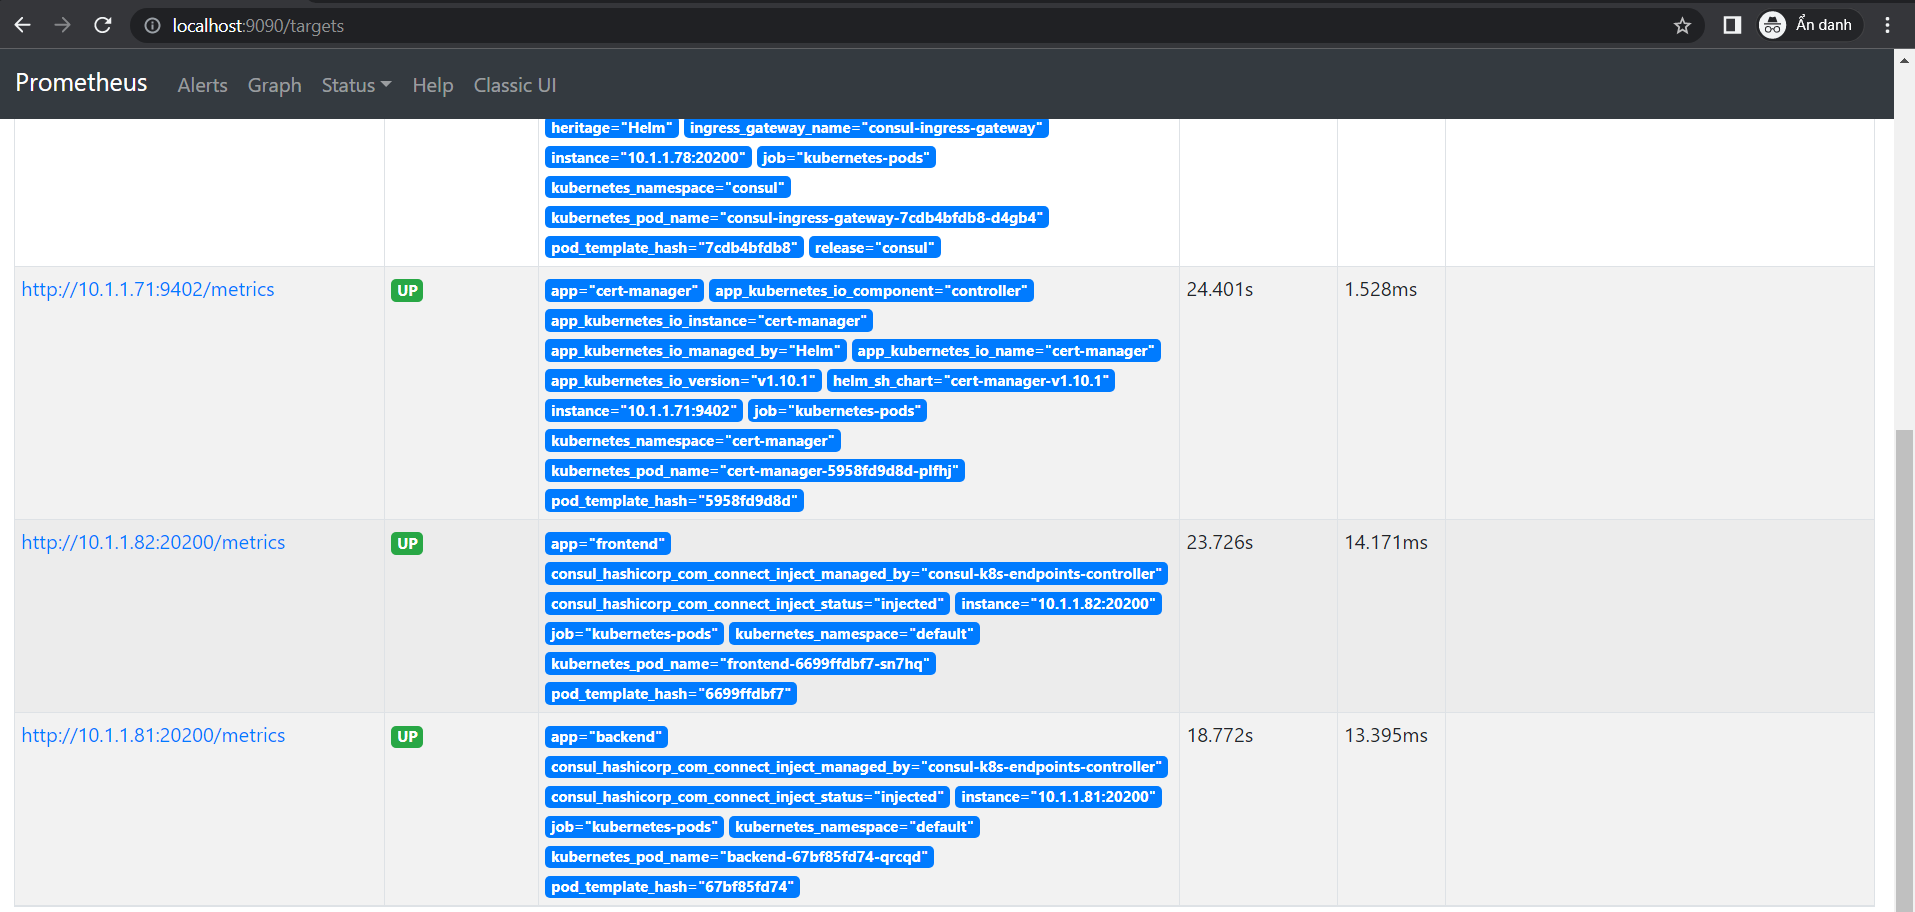
\includegraphics[width=1\linewidth]{Pics/target}
		\caption{\label{fig:target} Mục tiêu mà Prometheus đã thu thập được các metric.}
		\label{fig:target}
	\end{figure}
	\hspace{0.3cm}{Vậy là chúng ta đã đẩy được metrics lên trên Prometheus. Tiếp theo, chúng ta sẽ kiểm tra các metrics được hiện ở UI của Consul.}
	\begin{figure}[h]
	\centering
	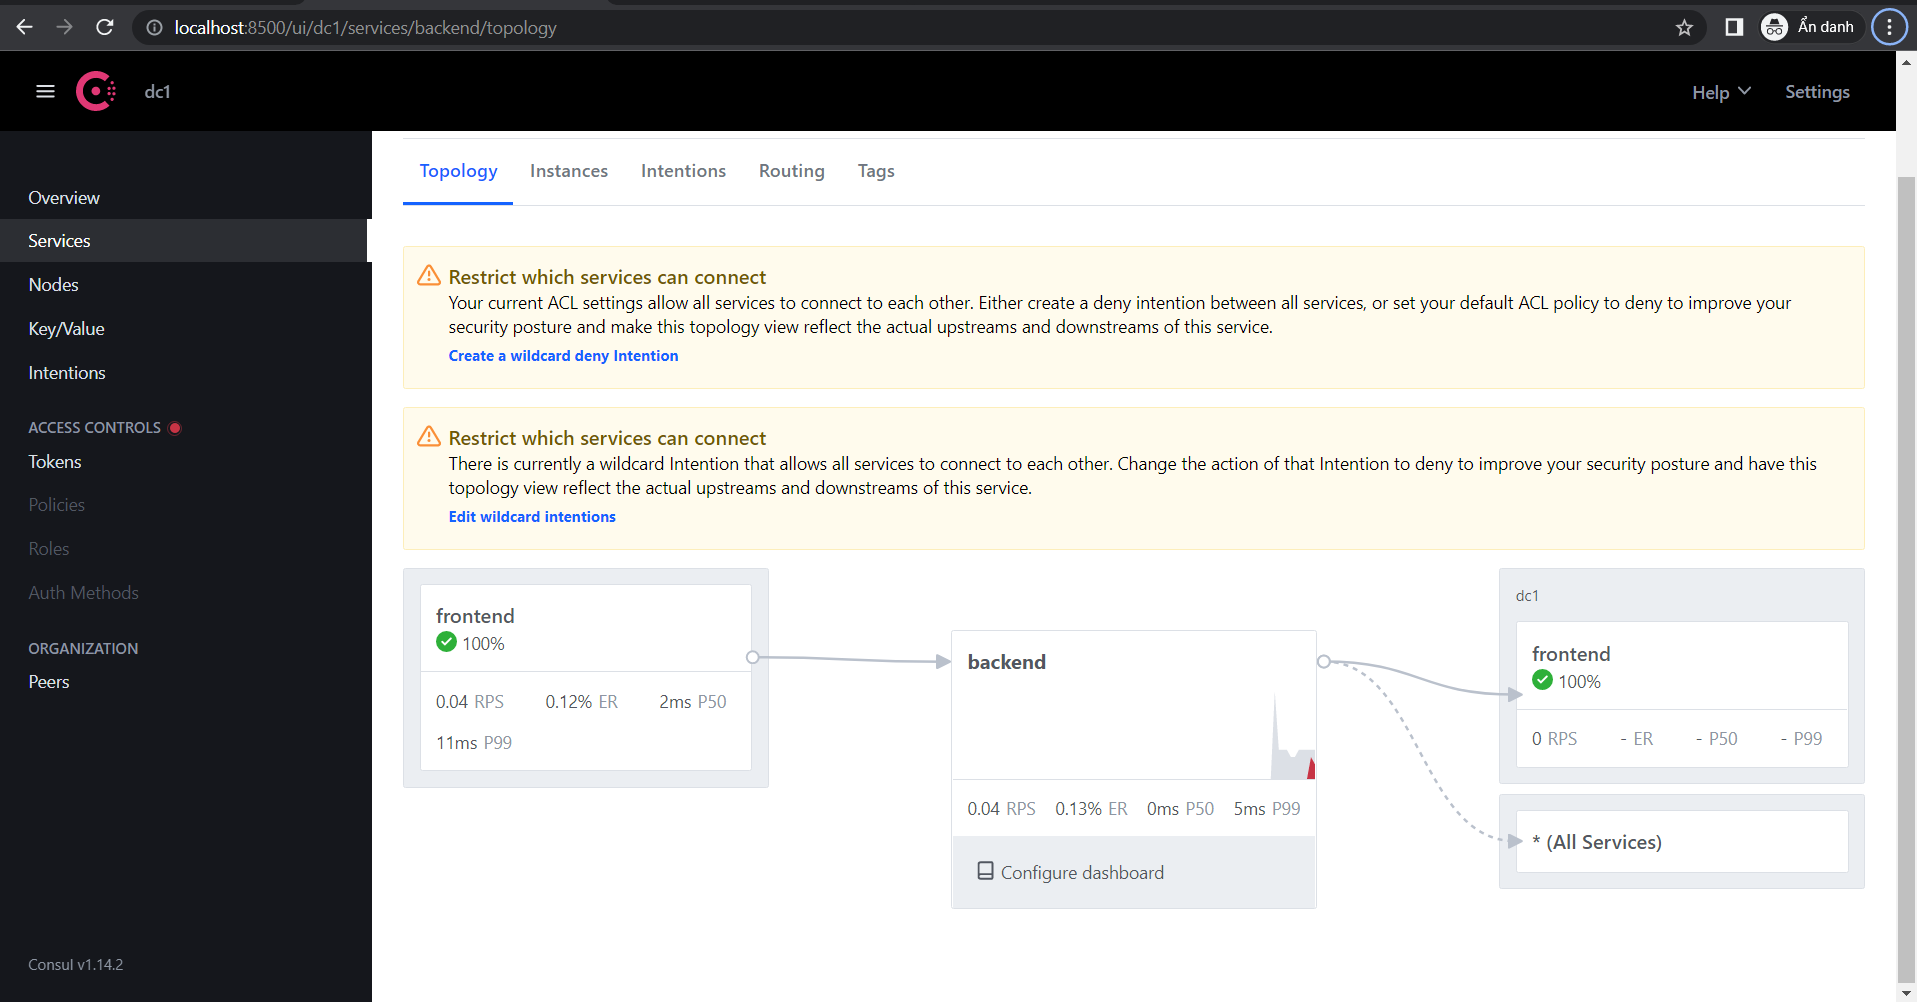
\includegraphics[width=1\linewidth]{Pics/ui-metrics}
	\caption{\label{fig:ui-metrics} Metrics hiện trên UI của Consul.}
	\label{fig:ui-metrics}
	\end{figure}
	\hspace{0.3cm}{Như vậy, chỉ việc nhìn vào cấu trúc hướng đi của các dịch vụ, chúng ta có thể nhìn thấy được các thông tin cụ thể mà metrics cung cấp trên màn hình. Điều này sẽ giúp cho việc kiểm tra và đánh giá tổng quát một cách nhanh nhất khi chúng ta có nhiều service được triển khai trên Kubernetes. \\}
	\hspace{0.3cm}{Tuy nhiên, khi mà dịch vụ không thể truy cập được, để điều tra nguyên nhân, chúng ta cần phải có một vài công cụ cụ thể hơn để có thể điều ra rõ nguồn gốc vấn đề. Để làm điều này, chúng ta sẽ triển khai thêm Jaeger, Jaeger là một công cụ giúp chúng ta điều tra cụ thể các luồng đi của dữ liệu. Để triển khai Jaeger, trước hết chúng ta cần cài đặt cert manager. Cert manager là một trong những điều kiện tiên quyết để cài đặt Jaeger. Để cài đặt Cert Manager, chúng ta cần chạy các lệnh sau:}
	\begin{lstlisting}[language=Bash]
	$ helm repo add jetstack https://charts.jetstack.io
	
	$ helm repo update
	
	$ kubectl apply -f https://github.com/cert-manager/cert-manager/releases/download/v1.10.1/cert-manager.crds.yaml
	
	$ helm install \
	cert-manager jetstack/cert-manager \
	--namespace cert-manager \
	--create-namespace \
	--version v1.10.1 \
	# --set installCRDs=true
	\end{lstlisting}
	\hspace{1.0cm}{Sau khi chạy thành công, Cert Manager đã được triển khai thành công trên kubernetes. Để kiểm tra, chúng ta sử dụng câu lệnh sau:}
	\begin{lstlisting}[language=Bash]
	$ kubectl get all -n cert-manager
	NAME                                           READY   STATUS    RESTARTS       AGE
	pod/cert-manager-5958fd9d8d-plfhj              1/1     Running   2 (3h1m ago)   2d22h
	pod/cert-manager-cainjector-7999df5dbc-h5kfl   1/1     Running   4 (3h ago)     2d22h
	pod/cert-manager-webhook-7f8f79d49c-qzkmk      1/1     Running   3 (3h1m ago)   2d22h
	
	NAME                           TYPE        CLUSTER-IP     EXTERNAL-IP   PORT(S)    AGE
	service/cert-manager           ClusterIP   10.103.15.91   <none>        9402/TCP   2d22h
	service/cert-manager-webhook   ClusterIP   10.111.32.49   <none>        443/TCP    2d22h
	
	NAME                                      READY   UP-TO-DATE   AVAILABLE   AGE
	deployment.apps/cert-manager              1/1     1            1           2d22h
	deployment.apps/cert-manager-cainjector   1/1     1            1           2d22h
	deployment.apps/cert-manager-webhook      1/1     1            1           2d22h
	
	NAME                                                 DESIRED   CURRENT   READY   AGE
	replicaset.apps/cert-manager-5958fd9d8d              1         1         1       2d22h
	replicaset.apps/cert-manager-cainjector-7999df5dbc   1         1         1       2d22h
	replicaset.apps/cert-manager-webhook-7f8f79d49c      1         1         1       2d22h
	\end{lstlisting}
	\hspace{1.0cm}{Tiếp theo đấy, chúng ta bắt đầu triển khai Jaeger. Để triển khai Jaeger, chúng ta cần chạy câu lệnh sau:}
	\begin{lstlisting}[language=Bash]
	$ kubectl create namespace observability
	$ kubectl apply -f https://github.com/jaegertracing/jaeger-operator/releases/download/v1.40.0/jaeger-operator.yaml
	customresourcedefinition.apiextensions.k8s.io/jaegers.jaegertracing.io created
	serviceaccount/jaeger-operator created
	role.rbac.authorization.k8s.io/leader-election-role created
	role.rbac.authorization.k8s.io/prometheus created
	clusterrole.rbac.authorization.k8s.io/jaeger-operator-metrics-reader created
	clusterrole.rbac.authorization.k8s.io/manager-role created
	clusterrole.rbac.authorization.k8s.io/proxy-role created
	rolebinding.rbac.authorization.k8s.io/leader-election-rolebinding created
	rolebinding.rbac.authorization.k8s.io/prometheus created
	clusterrolebinding.rbac.authorization.k8s.io/jaeger-operator-proxy-rolebinding created
	clusterrolebinding.rbac.authorization.k8s.io/manager-rolebinding created
	service/jaeger-operator-metrics created
	service/jaeger-operator-webhook-service created
	deployment.apps/jaeger-operator created
	certificate.cert-manager.io/jaeger-operator-serving-cert created
	issuer.cert-manager.io/jaeger-operator-selfsigned-issuer created
	mutatingwebhookconfiguration.admissionregistration.k8s.io/jaeger-operator-mutating-webhook-configuration created
	validatingwebhookconfiguration.admissionregistration.k8s.io/jaeger-operator-validating-webhook-configuration created
	\end{lstlisting}
	\hspace{1.0cm}{Tiếp theo, chúng ta sẽ tạo 1 tệp tin để tạo 1 ứng dụng Jaeger, pod loại Jaeger, ứng dụng này sẽ thu thập dữ liệu được gửi lên từ ứng dụng frontend và backend. Nội dung của tệp tin như sau:}
	\begin{lstlisting}[language=Bash]
	apiVersion: jaegertracing.io/v1
	kind: Jaeger
	metadata:
		name: jaeger
	spec:
		query:
			serviceType: LoadBalancer
		ingress:
			enabled: false
	\end{lstlisting}
	\hspace{1.0cm}{Sau khi tạo xong, thì Jaeger sẽ tạo cho chúng ta một deployment và giúp chúng ta có UI để truy vấn các dữ liệu. Để truy cập được UI, chúng ta cần port-forward cổng 16686 và bắt đầu truy cập vào \textit{http://localhost:16686} để xem thông tin query.}
	\begin{figure}[h]
		\centering
		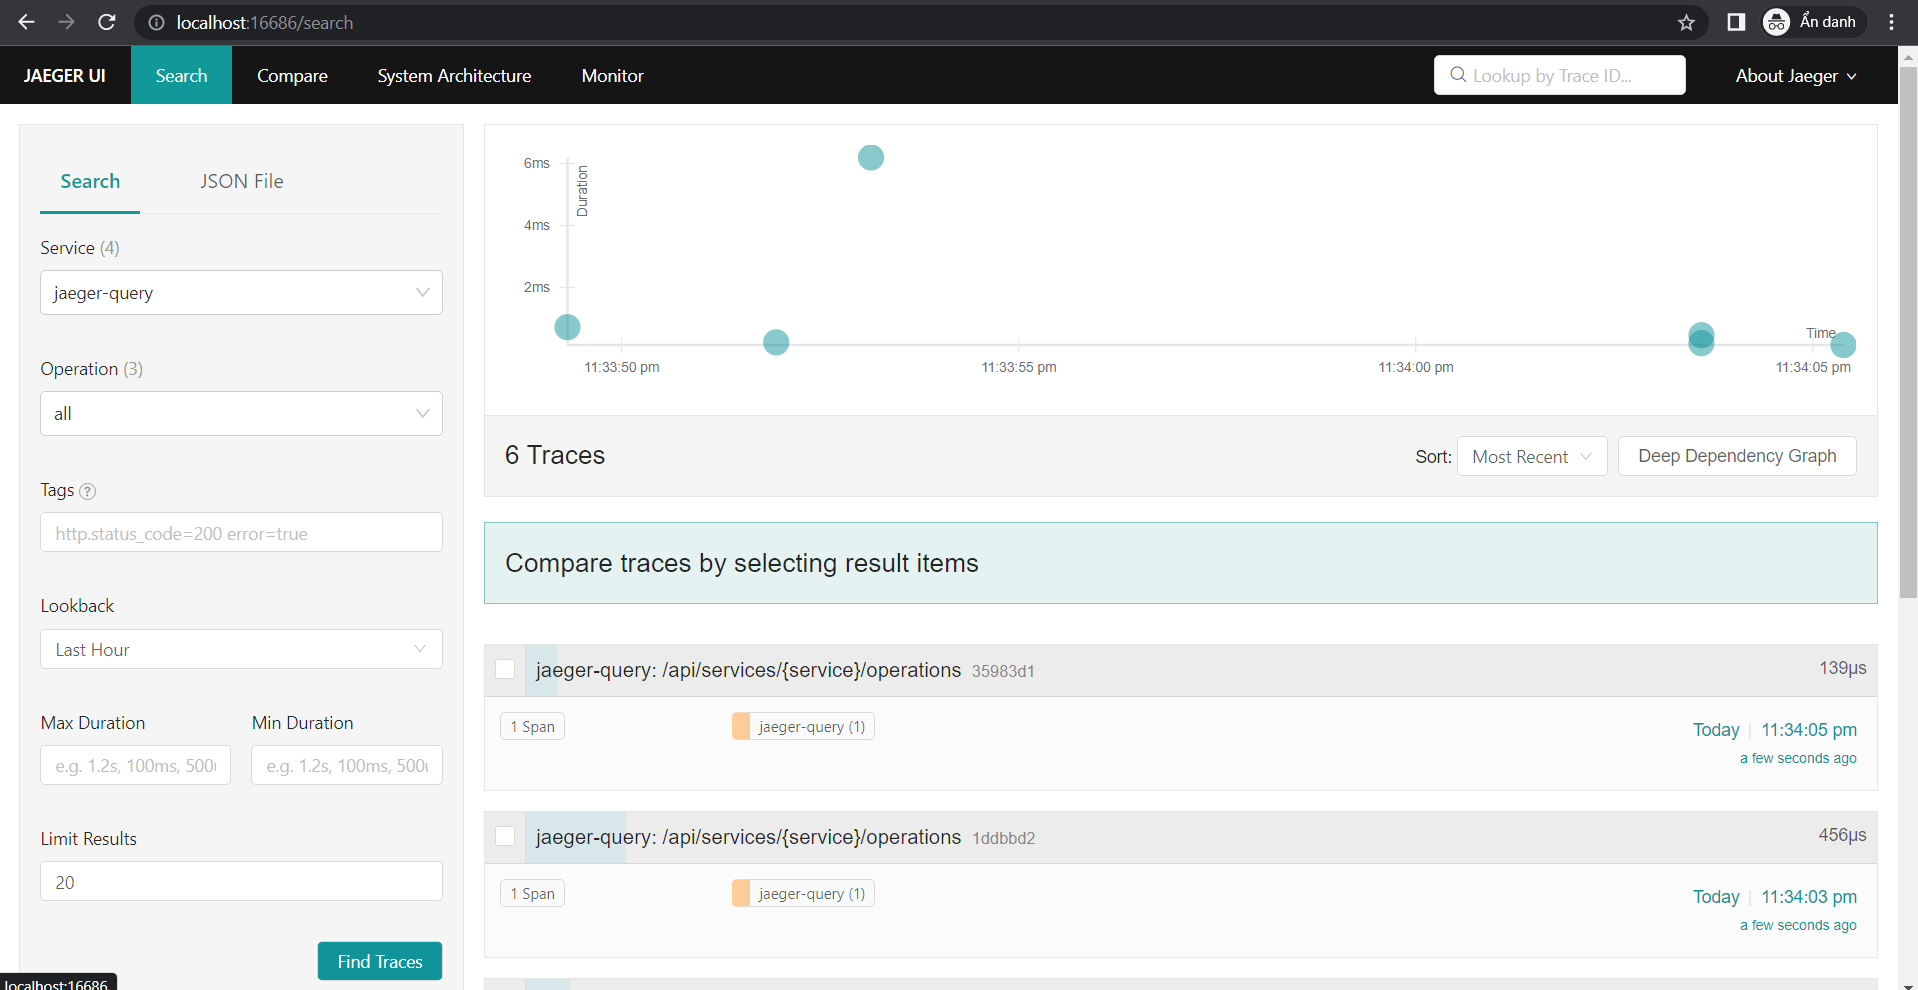
\includegraphics[width=1\linewidth]{Pics/jaeger-ui}
		\caption{\label{fig:jaeger-ui} UI của Jaeger.}
		\label{fig:jaeger-ui}
	\end{figure}
	\hspace{0.3cm}{Tiếp theo, chúng ta tiến hành đẩy dữ liệu từ ứng dụng frontend, backend và Proxy lên Jaeger. Để làm được điều này, chúng ta cần can thiệp vào trong code của ứng dụng. Tuy nhiên, ứng dụng frontend và backend đã được cấu hình để có thể đẩy dữ liệu ứng dụng lên trên Jaeger nên chúng ta chỉ việc khai báo thêm biến môi trường cho ứng dụng và ứng dụng sẽ đẩy dữ liệu lên. Còn đối với Proxy, chúng ta cần cấu hình lại một chút như sau:}
	\begin{lstlisting}[language=Bash]
	apiVersion: consul.hashicorp.com/v1alpha1
	kind: ProxyDefaults
	metadata:
		name: global
		namespace: consul
	spec:
		config:
			protocol: http
			envoy_tracing_json: |
			{
				"http":{
					"name":"envoy.tracers.zipkin",
					"typedConfig":{
						"@type":"type.googleapis.com/envoy.config.trace.v3.ZipkinConfig",
						"collector_cluster":"jaeger_collector",
						"collector_endpoint_version":"HTTP_JSON",
						"collector_endpoint":"/api/v2/spans",
						"shared_span_context":false
					}
				}
			}
			envoy_extra_static_clusters_json: |
			{
				"connect_timeout":"3.000s",
				"dns_lookup_family":"V4_ONLY",
				"lb_policy":"ROUND_ROBIN",
				"load_assignment":{
					"cluster_name":"jaeger_collector",
					"endpoints":[
					{
						"lb_endpoints":[
						{
							"endpoint":{
								"address":{
									"socket_address":{
										"address":"jaeger-collector.default",
										"port_value":9411,
										"protocol":"TCP"
									}
								}
							}
						}
						]
					}
					]
				},
				"name":"jaeger_collector",
				"type":"STRICT_DNS"
			}
	\end{lstlisting}
	\hspace{1.0cm}{Sau khi apply lại, thì chúng ta sẽ lên giao diện của Jaeger và kiểm tra: \\}
	\begin{figure}[h]
		\centering
		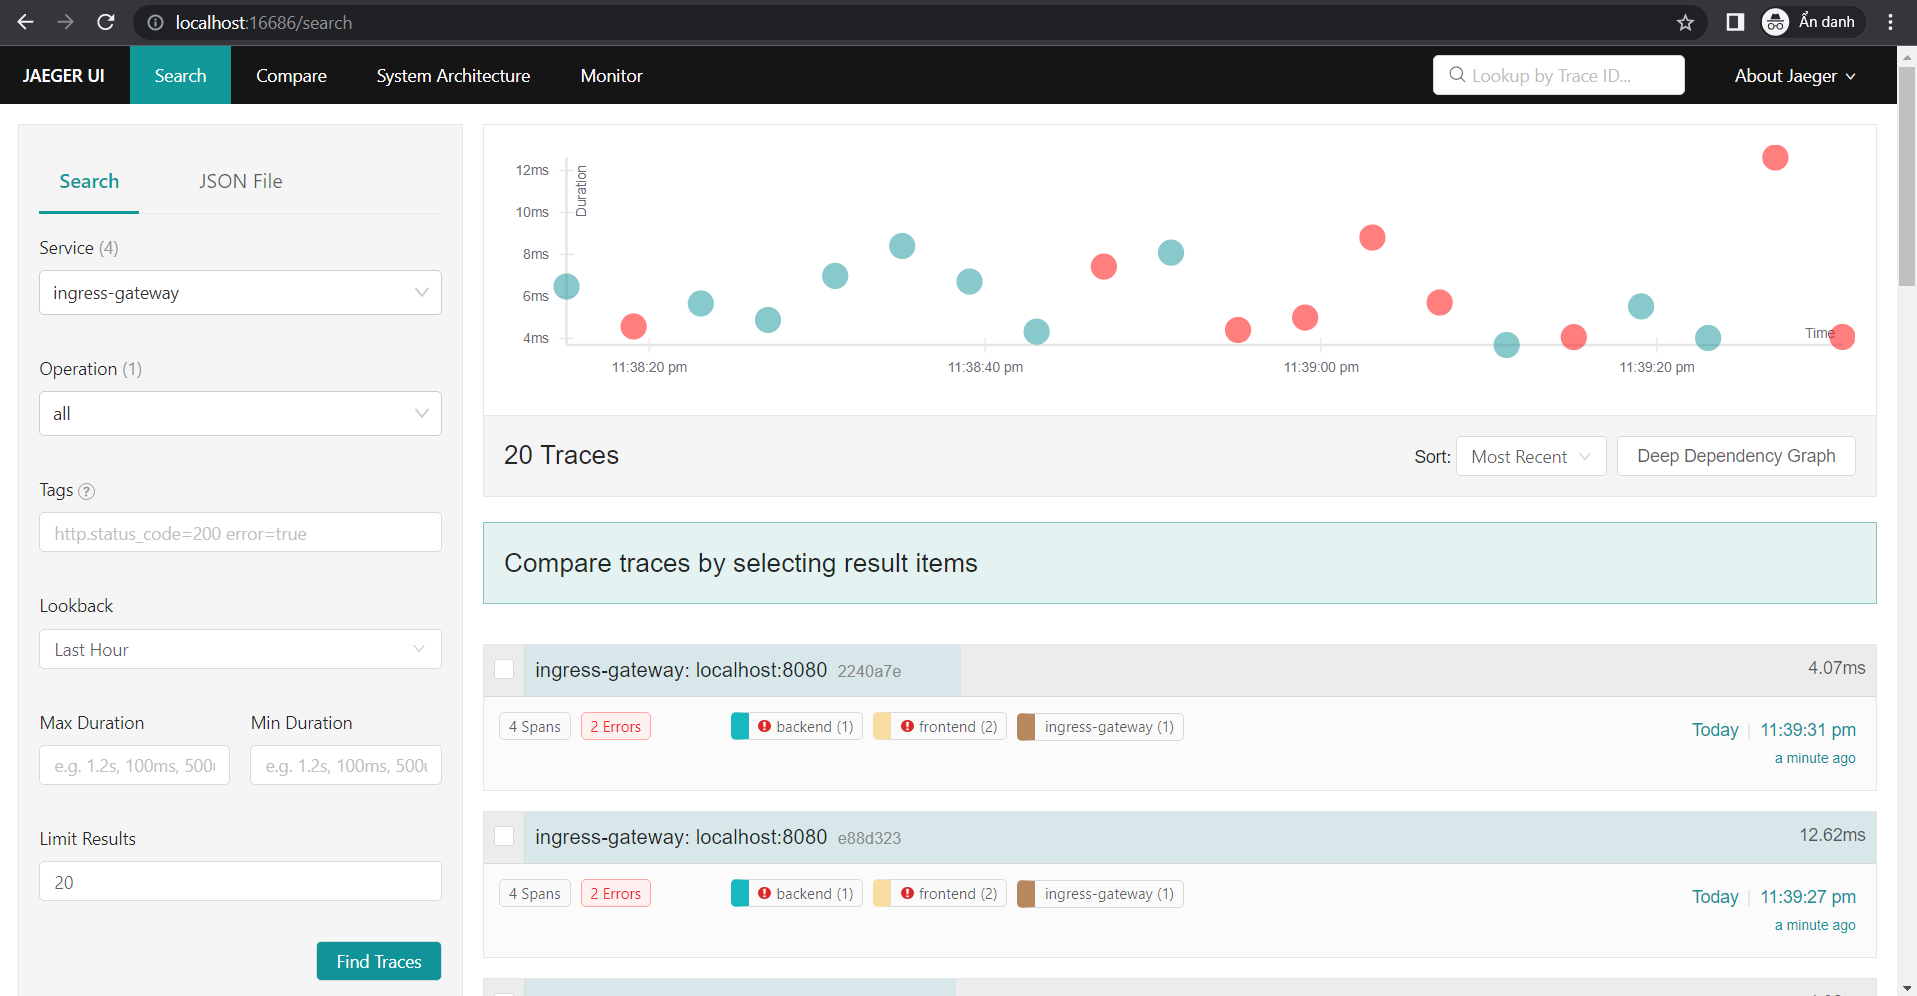
\includegraphics[width=1\linewidth]{Pics/jaeger-ingress-gateway}
		\caption{\label{fig:jaeger-ingress-gateway} Proxy đẩy dữ liệu lên Jaeger.}
		\label{fig:jaeger-ingress-gateway}
	\end{figure}
	\hspace{0.3cm}{Để điều tra, chúng ta sẽ ấn vào từng truy vấn cụ thể, và qua đấy, chúng ta sẽ biết được rằng nguyên nhân nào gây ra lỗi của ứng dụng.\\}
	\pagebreak
	\begin{figure}[h]
		\centering
		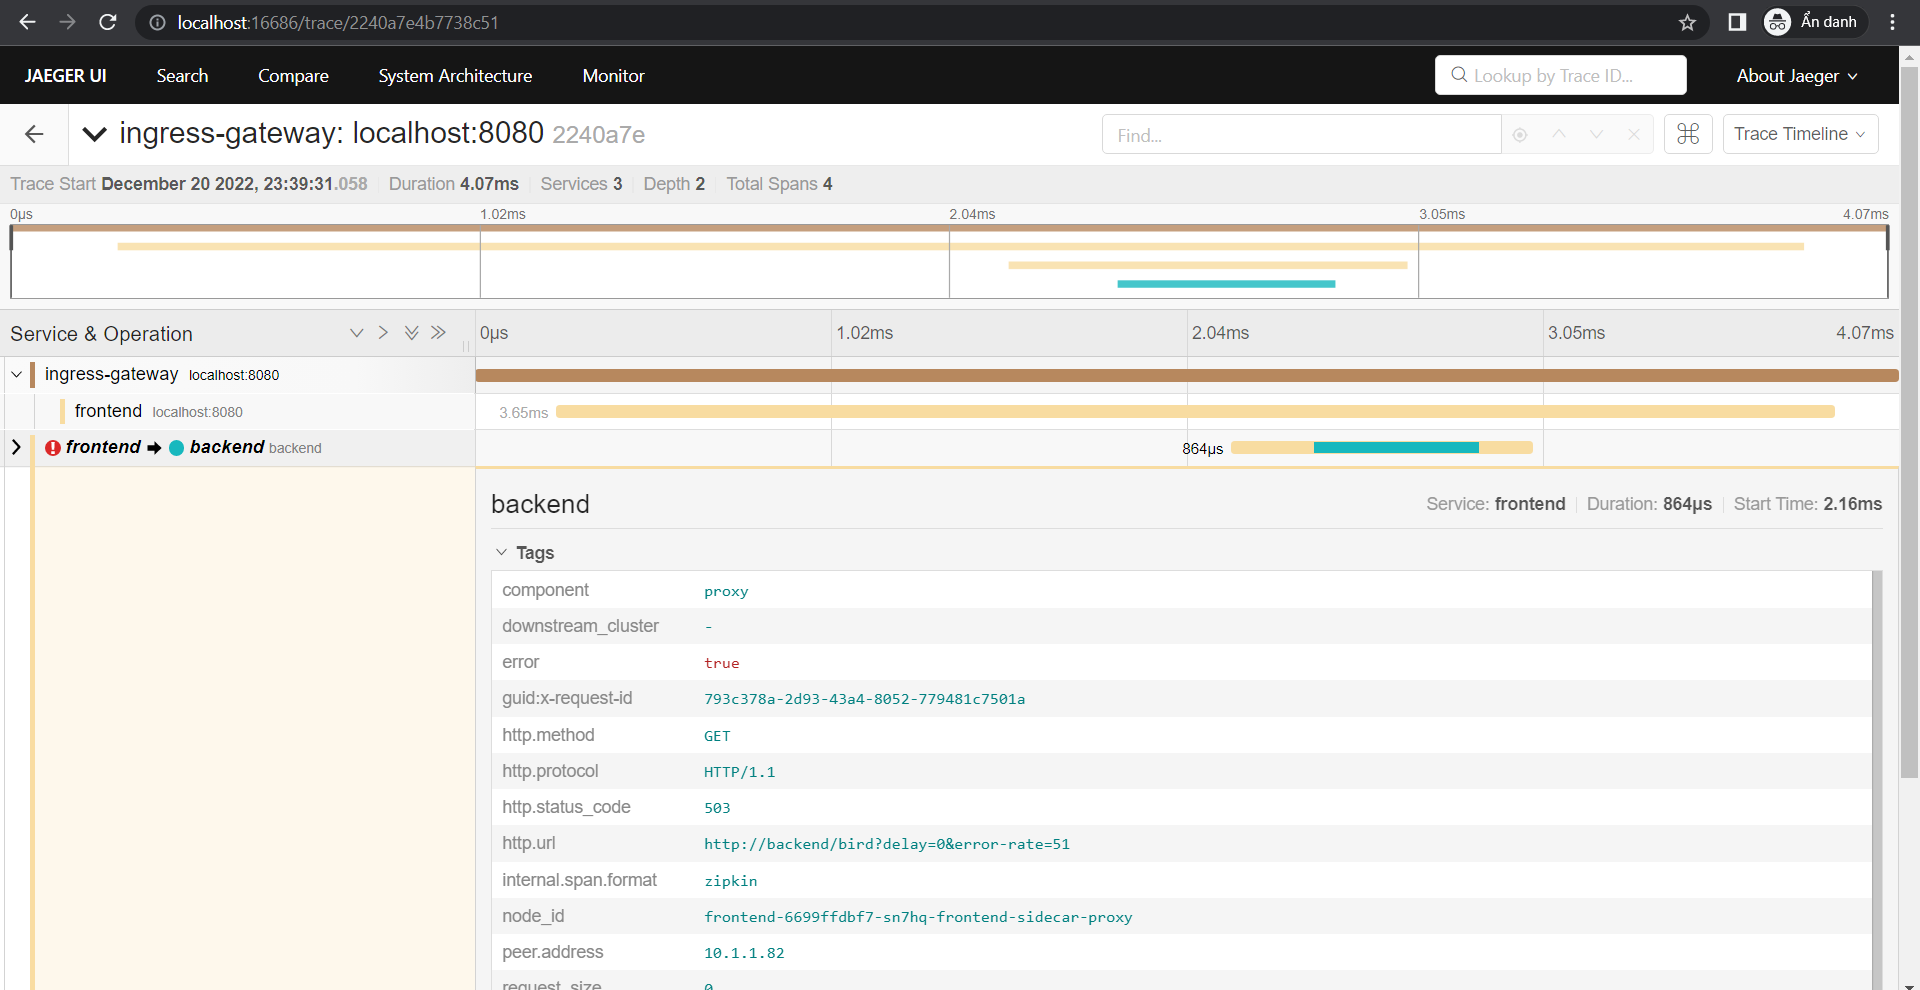
\includegraphics[width=1\linewidth]{Pics/jaeger-error}
		\caption{\label{fig:jaeger-error} Nguyên nhân lỗi đến từ backend.}
		\label{fig:jaeger-error}
	\end{figure}
	\subsubsection{Đánh giá}
	\hspace{0.3cm}{Vậy là chúng ta đã triển khai được hệ thống tracing và mở ra các metrics để có thể giúp chúng ta dễ dàng tiếp cận được những lỗi của ứng dụng. Tìm được nguyên nhân gây ra lỗi nhanh nhất có thể để làm giảm thời gian mất kết nối của hệ thống. Để triển khai phần này, thì sẽ tốn khá nhiều công sức, nhưng bù lại, khi chúng ta tìm nguyên nhân sẽ dễ dàng hơn rất nhiều vì chúng ta đã có đủ thông tin để tìm ra nguyên nhân gây ra lỗi.}
	\section*{Kết luận chương 3}
	\addcontentsline{toc}{section}{Kết luận chương 3}
	\hspace{1.0cm}{Qua chương 3, chúng ta đã thực hiện các phần thực nghiệm Consul trên Kubernetes. Qua các phần thực nghiệm này, chúng ta sẽ hiểu hơn về Consul hoạt động ra sao, vận hành như thế nào để giúp chúng ta có thể triển khai lên một cách chuẩn xác nhất và nhanh gọn nhất. Tuy nhiên, Consul vẫn nhiều tính năng mà chúng ta chưa triển khai vì phần này chúng ta chỉ tập chung vào tính năng service mesh trong consul. Vì vậy trong tương lai, chúng ta có thể tìm hiểu thêm các tính năng khác của consul và áp dụng được vào trong hệ thống kiến trúc của chúng ta.}
	\chapter*{\centering Lời kết thúc}
	\addcontentsline{toc}{chapter}{Lời kết thúc}
	\hspace{1.0cm}{Qua phần tìm hiểu trên, chúng ta đã tìm hiểu được nguyên lý hoạt động của Mircoservice, cách thức quản trị các Microservice trong Kubernetes. Qua đó, chúng ta đã nhìn thấy được tầm quan trọng của vấn đề bảo mật của Microservice trong Kubernetes. Và thứ có thể giúp chúng ta bảo mật các Microservice mà không cần phải chỉnh sửa lại code của ứng dụng đó chính là Service Mesh. Service Mesh giúp cho người quản trị có thể quản lý các Micorservice dễ dàng hơn, tăng tốc độ điều tra khi các Microservice bị lỗi, bảo mật giao tiếp giữa các Microservice. Và công cụ giúp chúng ta triển khai Service Mesh chính là Consul. Consul mặc dù tuổi đời không lâu, nhưng nó hiện đang là một trong các công cụ giúp cho người quản trị có thể dễ dàng triển khai Service Mesh lên Kubernetes để quản trị các Microservice trong Kubernetes.\\}
	
	\hspace{0.3cm}{Qua phần thực nghiệm, chúng ta đã tìm hiểu được cách thức hoạt động của Consul cũng như cách có thể vận hành Consul một cách cơ bản nhất. Tuy nhiên, Consul vẫn còn một vài điểm yếu cần phải khắc phục như là Ingress Gateway hiện tại chưa có tích hợp các chứng chỉ từ bên thứ ba và Consul là không phải OpenSource. Vì vậy Consul hiện giờ vẫn đang là một trong ít lựa chọn trong các doanh nghiệm hiện nay.}
	\chapter*{Tài liệu kham khảo}
	\section*{Consul: Up and Running}
	\section*{Microservice Security In Action}
	\section*{https://developer.hashicorp.com/consul/docs}
	\section*{https://github.com/hashicorp/consul-k8s}
	\section*{https://github.com/consul-up/examples}
	\section*{https://www.jaegertracing.io/}

\end{document}